% ******************************* PhD Thesis Template **************************
% Please have a look at the README.md file for info on how to use the template

\documentclass[a4paper,12pt,times,numbered,print,index,chapter]{Classes/PhDThesisPSnPDF}

% ******************************************************************************
% ******************************* Class Options ********************************
% *********************** See README for more details **************************
% ******************************************************************************

% `a4paper'(The University of Cambridge PhD thesis guidelines recommends a page
% size a4 - default option) or `a5paper': A5 Paper size is also allowed as per
% the Cambridge University Engineering Deparment guidelines for PhD thesis
%
% `11pt' or `12pt'(default): Font Size 10pt is NOT recommended by the University
% guidelines
%
% `oneside' or `twoside'(default): Printing double side (twoside) or single
% side.
%
% `print': Use `print' for print version with appropriate margins and page
% layout. Leaving the options field blank will activate Online version.
%
% `index': For index at the end of the thesis
%
% `draftclassic': For draft mode without loading any images (same as draft in book)
%
% `draft': Special draft mode with line numbers, images, and water mark with
% timestamp and custom text. Position of the text can also be modified.
%
% `abstract': To generate only the title page and abstract page with
% dissertation title and name, to submit to the Student Registry
%
% `chapter`: This option enables only the specified chapter and it's references
%  Useful for review and corrections.
%
% ************************* Custom Page Margins ********************************

% `custommargin`: Use `custommargin' in options to activate custom page margins,
% which can be defined in the preamble.tex. Custom margin will override
% print/online margin setup.
%
% *********************** Choosing the Fonts in Class Options ******************
%
% `times' : Times font with math support. (The Cambridge University guidelines
% recommend using times)
%
% `fourier': Utopia Font with Fourier Math font (Font has to be installed)
%            It's a free font.
%
% `customfont': Use `customfont' option in the document class and load the
% package in the preamble.tex
%
% default or leave empty: `Latin Modern' font will be loaded.
%
% ********************** Choosing the Bibliography style ***********************
%
% `authoryear': For author-year citation eg., Krishna (2013)
%
% `numbered': (Default Option) For numbered and sorted citation e.g., [1,5,2]
%
% `custombib': Define your own bibliography style in the `preamble.tex' file.
%              `\RequirePackage[square, sort, numbers, authoryear]{natbib}'.
%              This can be also used to load biblatex instead of natbib
%              (See Preamble)
%
% **************************** Choosing the Page Style *************************
%
% `default (leave empty)': For Page Numbers in Header (Left Even, Right Odd) and
% Chapter Name in Header (Right Even) and Section Name (Left Odd). Blank Footer.
%
% `PageStyleI': Chapter Name next & Page Number on Even Side (Left Even).
% Section Name & Page Number in Header on Odd Side (Right Odd). Footer is empty.
%
% `PageStyleII': Chapter Name on Even Side (Left Even) in Header. Section Number
% and Section Name in Header on Odd Side (Right Odd). Page numbering in footer
\usepackage{amsmath,scalerel}
\newcommand{\squeezeup}{\vspace{-2.5mm}}
\DeclareMathOperator*{\Bigcdot}{\scalerel*{\cdot}{\bigodot}}
\raggedbottom

% ********************************** Preamble **********************************
% Preamble: Contains packages and user-defined commands and settings
% ******************************************************************************
% ****************************** Custom Margin *********************************

% Add `custommargin' in the document class options to use this section
% Set {innerside margin / outerside margin / topmargin / bottom margin}  and
% other page dimensions
\ifsetCustomMargin
  \RequirePackage[left=37mm,right=30mm,top=35mm,bottom=30mm]{geometry}
  \setFancyHdr % To apply fancy header after geometry package is loaded
\fi

% *****************************************************************************
% ******************* Fonts (like different typewriter fonts etc.)*************

% Add `customfont' in the document class option to use this section

\ifsetCustomFont
  % Set your custom font here and use `customfont' in options. Leave empty to
  % load computer modern font (default LaTeX font).
  %\RequirePackage{helvet}

  % For use with XeLaTeX
  %  \setmainfont[
  %    Path              = ./libertine/opentype/,
  %    Extension         = .otf,
  %    UprightFont = LinLibertine_R,
  %    BoldFont = LinLibertine_RZ, % Linux Libertine O Regular Semibold
  %    ItalicFont = LinLibertine_RI,
  %    BoldItalicFont = LinLibertine_RZI, % Linux Libertine O Regular Semibold Italic
  %  ]
  %  {libertine}
  %  % load font from system font
  %  \newfontfamily\libertinesystemfont{Linux Libertine O}
\fi
\DeclareUnicodeCharacter{00A0}{~}
% *****************************************************************************
% **************************** Custom Packages ********************************

% ************************* Algorithms and Pseudocode **************************

%\usepackage{algpseudocode}


% ********************Captions and Hyperreferencing / URL **********************

% Captions: This makes captions of figures use a boldfaced small font.
%\RequirePackage[small,bf]{caption}

\RequirePackage[labelsep=space,tableposition=top]{caption}
\renewcommand{\figurename}{Fig.} %to support older versions of captions.sty



% *************************** Graphics and figures *****************************

%\usepackage{rotating}
%\usepackage{wrapfig}

% Uncomment the following two lines to force Latex to place the figure.
% Use [H] when including graphics. Note 'H' instead of 'h'
%\usepackage{float}
%\restylefloat{figure}

% Subcaption package is also available in the sty folder you can use that by
% uncommenting the following line
% This is for people stuck with older versions of texlive
%\usepackage{sty/caption/subcaption}
\usepackage{subcaption}
\usepackage[section]{placeins}
\usepackage{esvect}

% ********************************** Tables ************************************
\usepackage{booktabs} % For professional looking tables
\usepackage{multirow}

%\usepackage{multicol}
%\usepackage{longtable}
%\usepackage{tabularx}


% *********************************** SI Units *********************************
\usepackage{siunitx} % use this package module for SI units


% ******************************* Line Spacing *********************************

% Choose linespacing as appropriate. Default is one-half line spacing as per the
% University guidelines

% \doublespacing
% \onehalfspacing
% \singlespacing


% ************************ Formatting / Footnote *******************************

% Don't break enumeration (etc.) across pages in an ugly manner (default 10000)
%\clubpenalty=500
%\widowpenalty=500

%\usepackage[perpage]{footmisc} %Range of footnote options


% *****************************************************************************
% *************************** Bibliography  and References ********************
\usepackage{notoccite}
%\usepackage{cleveref} %Referencing without need to explicitly state fig /table

% Add `custombib' in the document class option to use this section
\ifuseCustomBib
   \RequirePackage[square, sort, numbers, authoryear]{natbib} % CustomBib

% If you would like to use biblatex for your reference management, as opposed to the default `natbibpackage` pass the option `custombib` in the document class. Comment out the previous line to make sure you don't load the natbib package. Uncomment the following lines and specify the location of references.bib file

%\RequirePackage[backend=biber, style=numeric-comp, citestyle=numeric, sorting=nty, natbib=true]{biblatex}
%\bibliography{References/references} %Location of references.bib only for biblatex

\fi

% changes the default name `Bibliography` -> `References'
\renewcommand{\bibname}{References}


% ******************************** Roman Pages *********************************
% The romanpages environment set the page numbering to lowercase roman one
% for the contents and figures lists. It also resets
% page-numbering for the remainder of the dissertation (arabic, starting at 1).

\newenvironment{romanpages}{
  \setcounter{page}{1}
  \renewcommand{\thepage}{\roman{page}}}
{\newpage\renewcommand{\thepage}{\arabic{page}}}


% ******************************************************************************
% ************************* User Defined Commands ******************************
% ******************************************************************************

% *********** To change the name of Table of Contents / LOF and LOT ************

%\renewcommand{\contentsname}{My Table of Contents}
%\renewcommand{\listfigurename}{My List of Figures}
%\renewcommand{\listtablename}{My List of Tables}


% ********************** TOC depth and numbering depth *************************

\setcounter{secnumdepth}{2}
\setcounter{tocdepth}{2}


% ******************************* Nomenclature *********************************

% To change the name of the Nomenclature section, uncomment the following line

%\renewcommand{\nomname}{Symbols}


% ********************************* Appendix ***********************************

% The default value of both \appendixtocname and \appendixpagename is `Appendices'. These names can all be changed via:

%\renewcommand{\appendixtocname}{List of appendices}
%\renewcommand{\appendixname}{Appndx}

% *********************** Configure Draft Mode **********************************

% Uncomment to disable figures in `draftmode'
%\setkeys{Gin}{draft=true}  % set draft to false to enable figures in `draft'

% These options are active only during the draft mode
% Default text is "Draft"
%\SetDraftText{DRAFT}

% Default Watermark location is top. Location (top/bottom)
%\SetDraftWMPosition{bottom}

% Draft Version - default is v1.0
%\SetDraftVersion{v1.1}

% Draft Text grayscale value (should be between 0-black and 1-white)
% Default value is 0.75
%\SetDraftGrayScale{0.8}


% ******************************** Todo Notes **********************************
%% Uncomment the following lines to have todonotes.

%\ifsetDraft
%	\usepackage[colorinlistoftodos]{todonotes}
%	\newcommand{\mynote}[1]{\todo[author=kks32,size=\small,inline,color=green!40]{#1}}
%\else
%	\newcommand{\mynote}[1]{}
%	\newcommand{\listoftodos}{}
%\fi

% Example todo: \mynote{Hey! I have a note}

% ************************ Thesis Information & Meta-data **********************
% Thesis title and author information, refernce file for biblatex
% ************************ Thesis Information & Meta-data **********************
%% The title of the thesis
\title{Multi-microscopy Characterisation of III-nitride Devices and Materials}
%\texorpdfstring is used for PDF metadata. Usage:
%\texorpdfstring{LaTeX_Version}{PDF Version (non-latex)} eg.,
%\texorpdfstring{$sigma$}{sigma}

%% Subtitle (Optional)
%\subtitle{Using the CUED template}

%% The full name of the author
\author{Christopher Xiang Ren}

%% Department (eg. Department of Engineering, Maths, Physics)
\dept{Department of Materials Science and Metallurgy}

%% University and Crest
\university{University of Cambridge}
% Crest minimum should be 30mm.
\crest{
\includegraphics[width=0.2\textwidth]{University_Crest}}
%% Use this crest, if you are using the college crest
%% Crest long miminum should be 65mm
%\crest{
\includegraphics[width=0.45\textwidth]{University_Crest_Long}}

%% College shield [optional] 
% Crest minimum should be 30mm.
%\collegeshield{
\includegraphics[width=0.2\textwidth]{CollegeShields/Kings}}

%% You can redefine the submission text:
% Default as per the University guidelines:
% ``This dissertation is submitted for the degree of''
%\renewcommand{\submissiontext}{change the default text here if needed}

%% Full title of the Degree
\degreetitle{Doctor of Philosophy}

%% College affiliation (optional)
\college{Wolfson College}

%% Submission date
% Default is set as {\monthname[\the\month]\space\the\year}
%\degreedate{September 2014} 

%% Meta information
\subject{LaTeX} \keywords{{LaTeX} {PhD Thesis} {Materials Science and Metallurgy} {University of
Cambridge}}

% ***************************** Abstract Separate ******************************
% To printout only the titlepage and the abstract with the PhD title and the
% author name for submission to the Student Registry, use the `abstract' option in
% the document class.

\ifdefineAbstract
 \pagestyle{empty}
 \includeonly{Declaration/declaration, Abstract/abstract}
\fi

% ***************************** Chapter Mode ***********************************
% The chapter mode allows user to only print particular chapters with references
% Title, Contents, Frontmatter are disabled by default
% Useful option to review a particular chapter or to send it to supervisior.
% To use choose `chapter' option in the document class

\ifdefineChapter
 \includeonly{Chapter4/chapter4}
\fi

% ******************************** Front Matter ********************************
\setcounter{secnumdepth}{5}
\begin{document}

\frontmatter

\begin{titlepage}
  \maketitle
\end{titlepage}


% ******************************* Thesis Dedidcation ********************************

\begin{dedication} 

I would like to dedicate this thesis to my loving parents \dots

\end{dedication}
% ******************************* Thesis Declaration ***************************

\begin{declaration}

I hereby declare that except where specific reference is made to the work of 
others, the contents of this dissertation are original and have not been 
submitted in whole or in part for consideration for any other degree or 
qualification in this, or any other university. This dissertation is my own 
work and contains nothing which is the outcome of work done in collaboration 
with others, except as specified in the text and Acknowledgements. This 
dissertation contains fewer than 65,000 words including appendices, 
bibliography, footnotes, tables and equations and has fewer than 150 figures.

% Author and date will be inserted automatically from thesis.tex \author \degreedate

\end{declaration}
% ************************** Thesis Acknowledgements **************************

\begin{acknowledgements}      


And I would like to acknowledge ...


\end{acknowledgements}

% ************************** Thesis Abstract *****************************
% Use `abstract' as an option in the document class to print only the titlepage and the abstract.
\begin{abstract}
This is where you write your abstract ...
\end{abstract}


% *********************** Adding TOC and List of Figures ***********************

\tableofcontents

\listoffigures

\listoftables

%\printnomenclature[space] space can be set as 2em between symbol and description
\printnomenclature[9em]


% ******************************** Main Matter *********************************
\mainmatter

%*******************************************************************************
%*********************************** First Chapter *****************************
%*******************************************************************************

\chapter{Introduction}  %Title of the First Chapter

\ifpdf
    \graphicspath{{Chapter1/Figs/Raster/}{Chapter1/Figs/PDF/}{Chapter1/Figs/}}
\else
    \graphicspath{{Chapter1/Figs/Vector/}{Chapter1/Figs/}}
\fi

Gallium nitride \nomenclature[z-GaN]{GaN}{Gallium Nitride} (GaN) has been termed the 'most important semiconductor material since silicon' \cite{Humphreys2008}, and indeed the influence of this incredible material and it's associated alloys (termed III-nitrides) is pervasive in modern society. The impact of III-nitride materials is perhaps best evidenced by the global transition from traditional lighting sources to semiconductor lighting solutions based on III-nitride materials. Since the first demonstration of a high-brightness blue light emitting diode \nomenclature[z-LED]{LED}{Light-Emitting Diode} (LED) in 1991 by Shuji Nakamura \cite{Nakamura1991}, the widespread use of LEDs for general lighting purposes has blossomed into a multi-billion pound industry. The extraordinary optical properties of III-nitride materials have enabled their application outside of the lighting industry: the development of III-nitride based lasers has found applications in telecommunications \cite{Najda2015}, medicine \cite{BerlienBreuerMuellerEtAl2012} and data storage . Furthermore, III-nitride optical emitters have been used as single photon sources \nomenclature[z-SPS]{SPS}{Single Photon Source} (SPSs) which have applications in cryptography for secure communications \cite{Kako2006}.
\\The optoelectronic properties of III-nitride materials are somewhat astonishing: GaN suffers from a defect density several orders of magnitude higher than other optically active semiconductor materials such as gallium arsenide \nomenclature[z-GaAs]{GaAs}{Gallium Arsenide} (GaAs) \cite{Bennett2010b} yet is still optically active. Despite this, the effects of defects originating from the heteropitaxial growth of GaN are clearly deleterious when considering III-nitride device operation. 
This work aims to explore the manner in which the microstructural properties of photonic III-nitride devices affect their performance by combining multiple microscopy techniques, an approach we term 'multi-microscopy', thus allowing us to link specific structural features with emissive properties at the device level. The experimental research in this thesis is separated into four main sections. 
\\The first section details the investigation of inhomogeneous electroluminescence \nomenclature[z-EL]{EL}{Electroluminescence} (EL) of indium gallium nitride (InGaN) quantum well (QW) LEDs. By employing the use of scanning probe techniques, electron microscopy and spectroscopy the underpinning cause of LED behaviour was elucidated and reported.
\\The second section involves microscopy-based investigation into the mechanisms behind incomplete etching in the fabrication of III-nitride based microdisk cavities and the effect of this issue on the overall optical performance of these cavities
\\The third section describes the microscopy of one dimensional \nomenclature[z-1-D]{1-D}{One-Dimensional} (1-D) photonic crystal cavity (PCC) 'nanobeam' cavities. The intrinsic resistance of III-nitride based materials can often result in improperly etched features, which can results in high optical losses in cavities. This section concerns the use of tomographic techniques such as electron tomography \nomenclature[z-ET]{ET}{Electron Tomography} (ET) and focussed ion beam tomography \nomenclature[z-FIBT]{FIBT}{Focussed Ion Beam Tomography} (FIB-T) to investigate the effect of these issues on the emission of III-nitride nanobeam cavities. 

%********************************** %First Section  **************************************
\section{III-Nitride Material Properties } %Section - 1.1 

\subsection{Crystal Structure}
\label{section1.1.1}

GaN can crystallise into two distinct crystal structures: hexagonal (wurtzite) and cubic (zinc blende and rock salt). Under ambient conditions, wurtzite GaN is the most commonly studied form as it is the most structurally stable. Thus, the work discussed in this thesis concerns wurtzite III-nitrides. A schematic of a wurtzite III-nitride crystal structure is shown in Fig.\ref{1.1} and consists of stacked hexagonal close-packed planes following an ABABAB stacking sequence. Atoms of the respective elements are tetrahedrally bonded to one another. However, in the case of III-nitrides this structure deviates from ideal tetrahedral bonding and results in a non-zero dipole moment for each unit cell which will be discussed in the following sections.
\\ A 4-index Miller-Bravais notation (hkil) is used to denote the crystal planes where the index {\it i} is defined by the relation:

\begin{equation}
 i = -(h+k)
 \end{equation}
\\
 
The crystallographic planes (0001), (1-100) and (11-20) shown in Fig.\ref{1.1} are often termed the {\it c}, {\it m} and {\it a}-planes in the literature. The fundamental unit cell of the wurtzite GaN crystal structure and its associated lattice parameters \textbf{a} and \textbf{c} is shown in Fig.\ref{1.2}

\begin{figure}[h]
	\centering
	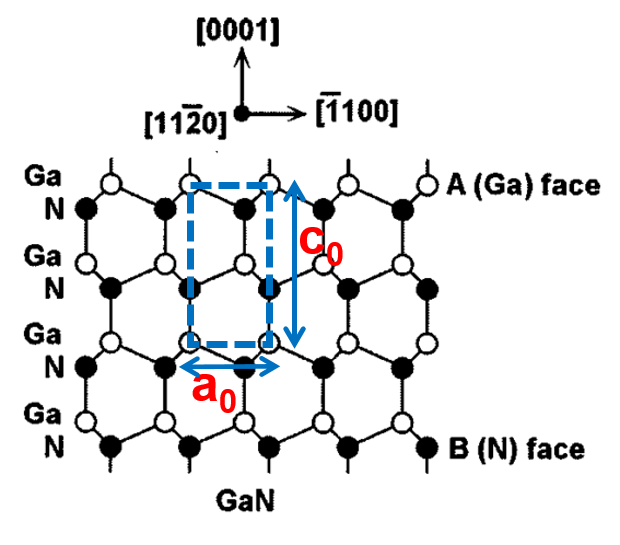
\includegraphics[width=0.5\textwidth]{Figs/Ch1/unit_cell.png}
	\caption {Unit cell (dashed line) for GaN crystal structure and lattice parameters $\mathbf{a_{0}},\mathbf{c_{0}}$. Adapted from \cite{Yu1999}}
	\label{1.2}
\end{figure}
\FloatBarrier

Other members of the III-nitride materials such as indium nitride \nomenclature[z-InN]{InN}{Indium Nitride} (InN) or aluminium nitride \nomenclature[z-AlN]{AlN}{Aluminium Nitride} (AlN) have different lattice parameters due to the differing atomic radii of aluminium and indium relative to gallium.

\begin{table}[!htb]
	\centering
	
	\begin{tabular}{ccc}
		Alloy & \textbf{a} (\si{\angstrom}) at T = 300K & \textbf{c} (\si{\angstrom}) at T = 300K \\
		%heading
		\hline\hline
		GaN   & 3.189   & 5.185   \\
		InN   & 3.545   & 5.703   \\
		AlN   & 3.112  & 4.982  \\ 
		\hline
	\end{tabular}
	\caption{Room temperature lattice parameters for GaN, InN and AlN \cite{Vurgaftman2003}.}
	\label{tab1.1}
\end{table}

III-nitride photonic devices are often heterostructures consisting of ternary alloys the materials shown in Table~\ref{tab1.1}. Lattice parameters of a relaxed ternary alloy $A_{x}B_{1-x}N$ can be estimated using Vegard's law \cite{Vickers2003}:

\begin{equation}
\mathbf{a} = x \mathbf{a}_{AN} + (1-x)\mathbf{a}_{BN}
\end{equation}

\begin{equation}
\mathbf{c} = x \mathbf{c}_{AN} + (1-x)\mathbf{c}_{BN}
\end{equation}

Typical indium compositions for blue LEDs range between 15-20 $\%$, which leads to a considerable lattice mismatch of approximately 2 $\%$, resulting in considerable amounts of strain in these GaN/InGaN heterostructures.

\subsection{Band Structure} 
\label{section1.1.2}

One of the principal driving factors behind the interest in III-nitrides for photonic devices is their direct bandgap which collectively spans the visible spectrum and beyond. The bandgap of III-nitride binary alloys is given below in Table.\ref{tab1.2}.

\begin{table}[!htb]
	\centering
	\begin{tabular}{cc}
		Alloy & Bandgap (eV) \\
		%heading
		\hline\hline
		GaN   & 3.51 \\
		InN   & 0.78 \\
		AlN   & 6.25  \\ 
		\hline
	\end{tabular}
	\caption{Direct bandgaps of GaN, InN and AlN \cite{Vurgaftman2003}.}
	\label{tab1.2}
\end{table}

Ternary alloying modifies the bandgap as shown in Fig.\ref{bgap}. In theory the entire range of 0.78-6.25 eV is accessible through alloying, though material limitations reduce the full effective range for III-nitride devices \cite{Scholz2012}.

\begin{figure}[h]
	\centering
	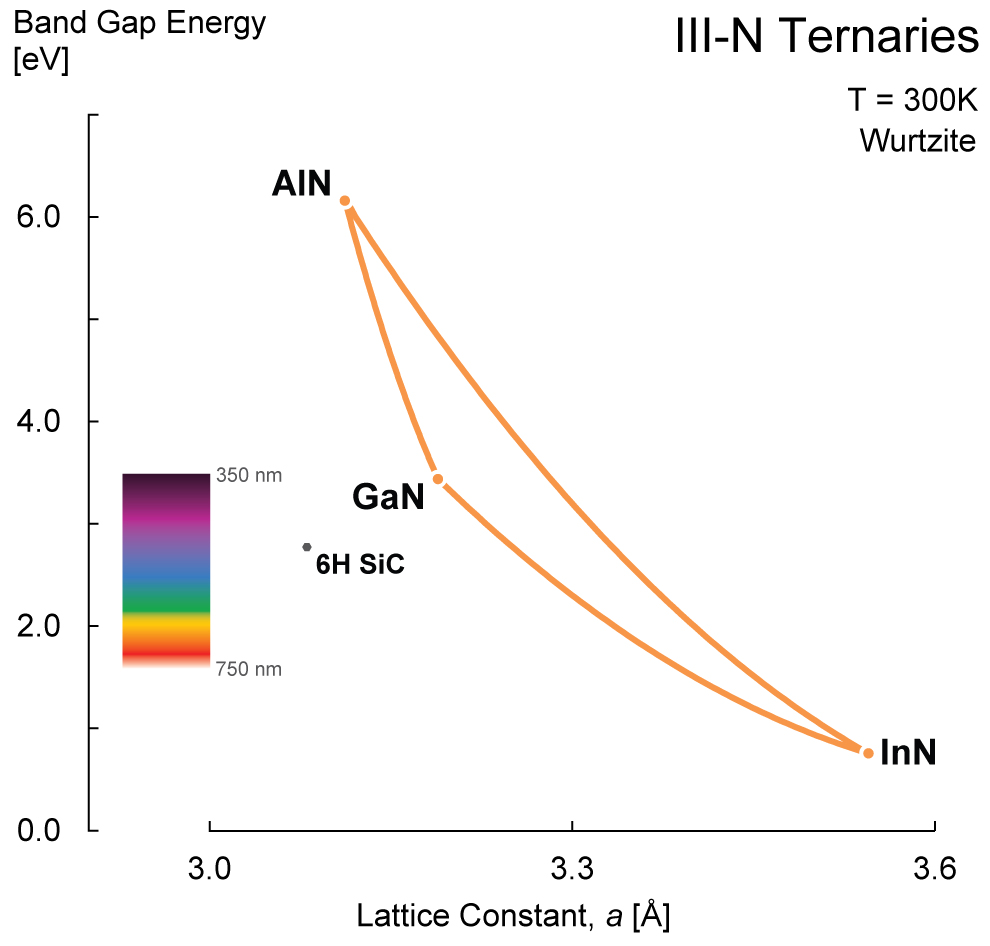
\includegraphics[width=0.7\textwidth]{Figs/Ch1/III-N-Ternaries-update.jpg}
	\caption {Bandgap at room temperature for III-nitride materials with the visible spectrum shown on the left. Courtesy of K. Montgomery.}
	\label{bgap}
\end{figure}
\FloatBarrier

The bandgap of a ternary alloy $A_{x}B_{1-x}N$ is given by a modified Vegard's Law:

\begin{equation}
E_{g} = x E_{g}^{AN} + (1-x)E_{g}^{BN}-x(1-x)C
\end{equation}

Where C is a bowing parameter which accounts for deviation from a linear relation between ternary alloy composition and bandgap energy. The value of the InGaN bowing parameter has been widely debated in the literature due to the lack of a reliable value for the bandgap energy for InN \cite{Vurgaftman2003}. Although the current value of 1.4 eV is reported, there are also suggestions the bowing parameter may be composition dependent \cite{Wu2002,McCluskey2003,Moses2010}.\\
In considering the optical properties of III-nitride materials it is also important to consider the effects of impurities and defects. Crystal disorder introduces further energy states which would be 'forbidden' in an ideal crystal lattice leading to an effective 'smearing' of the bandgap. Sub-bandgap absorption can occur due to the introduction of these defective states. The smearing out of the absorption edge of the material is known as the 'Urbach tail', and can be a highly deleterious source of loss in III-nitride cavity structures \cite{Puchtler2015}. 

\subsubsection{Quantum Confinement Effects}

The first prototype high-brightness blue III-nitride LED consisted of a GaN {\it p-n} junction, or a 'homojunction' \cite{Nakamura1991}, however modern LED structures consist of heterostructures known as quantum wells. QWs consist of a thin layer of low bandgap material between two quantum barriers with a higher bandgap. Carriers in the low bandgap material are effectively confined in one direction, hence the term 'quantum well'. This confinement leads to the discretisation of the carrier wavefunctions within the well, as shown schematically in Fig.\ref{QW}.

\begin{figure}[h]
	\centering
	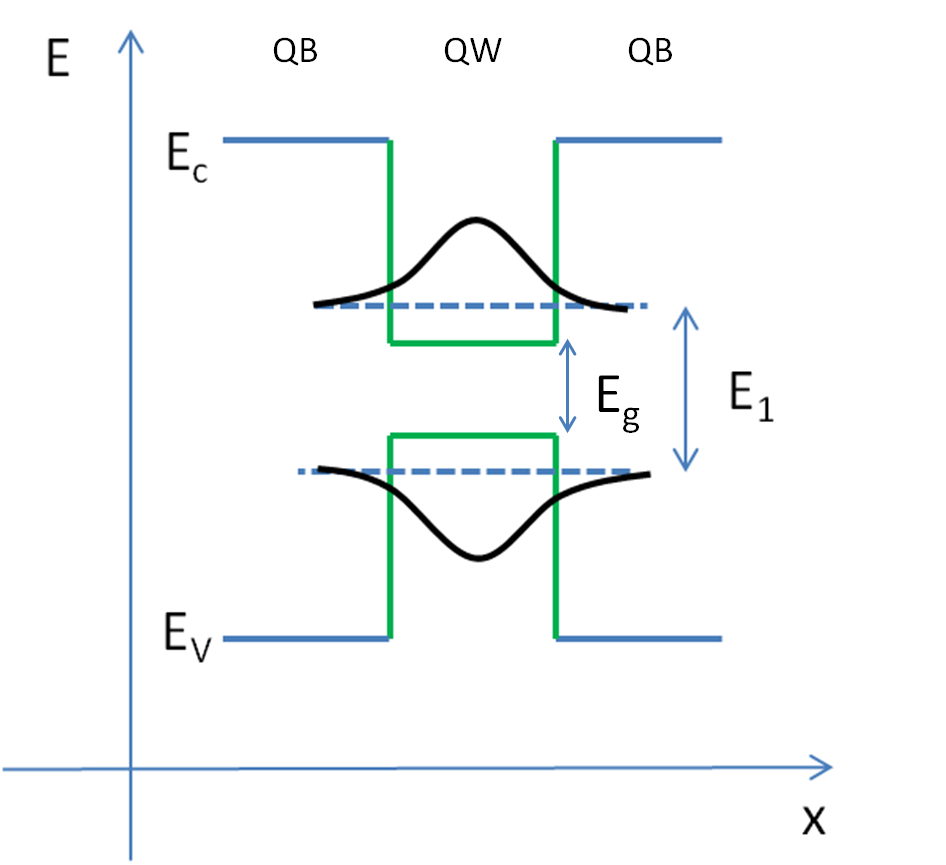
\includegraphics[width=0.5\textwidth, trim = 4 4 4 4 , clip]{Figs/Ch1/BandstructureQW.png}
	\caption {Band diagram of a quantum well. The bandgap of the well material is denoted $E_{g}$, the energy of the ground state transition is denoted $E_{1}$ and the conduction and valence bands are denoted $E_{c},E_{v}$ respectively \cite{Ren2015}.}
	\label{QW}
\end{figure}
\FloatBarrier

Thus the energy of the transition in the QW is given by the following relation:

\begin{equation}
h\nu = E_{1}-E_{ex}
\end{equation}

where $E_{1}$ is the energy of the ground state transition and $E_{ex}$ is the exciton binding energy. For an infinite potential well of thickness L, the ground state $E_{1}$ is given by:

\begin{equation}
E_{1}=\frac{\hbar^{2}\pi_{2}}{2m^{*}L^{2}}
\end{equation}

where $\hbar$ is the reduced Plank constant, $m^{*}$ is the carrier effective mass. As such, the energy of the optical transition can be related to the thickness of the well.





\subsection{Built-in Fields} 
\label{section1.1.3}
III-nitride materials in wurtzite structure are termed 'polar' materials, due to the fact they exhibit a spontaneous polarisation field \cite{Ambacher2002}. This occurs due to III-nitride bonding structure deviating from an ideal tetrahedral structure along the (0001) axis along the crystal, combined with the ionicity of the bond \cite{Ren2015}. This deviation causes each unit cell to possess a non-zero dipole moment along the principal axis of the tetrahedral bonding structure, resulting in an overall spontaneous polarization in the crystal. As the III-nitride wurtzite structure is non-centrosymmetric, the direction of the polarization depends on whether the crystal exhibits (+ {\it c}) or (-{\it c}) polarity, as shown in Fig.\ref{1.3}

\begin{figure}[h]
	\centering
	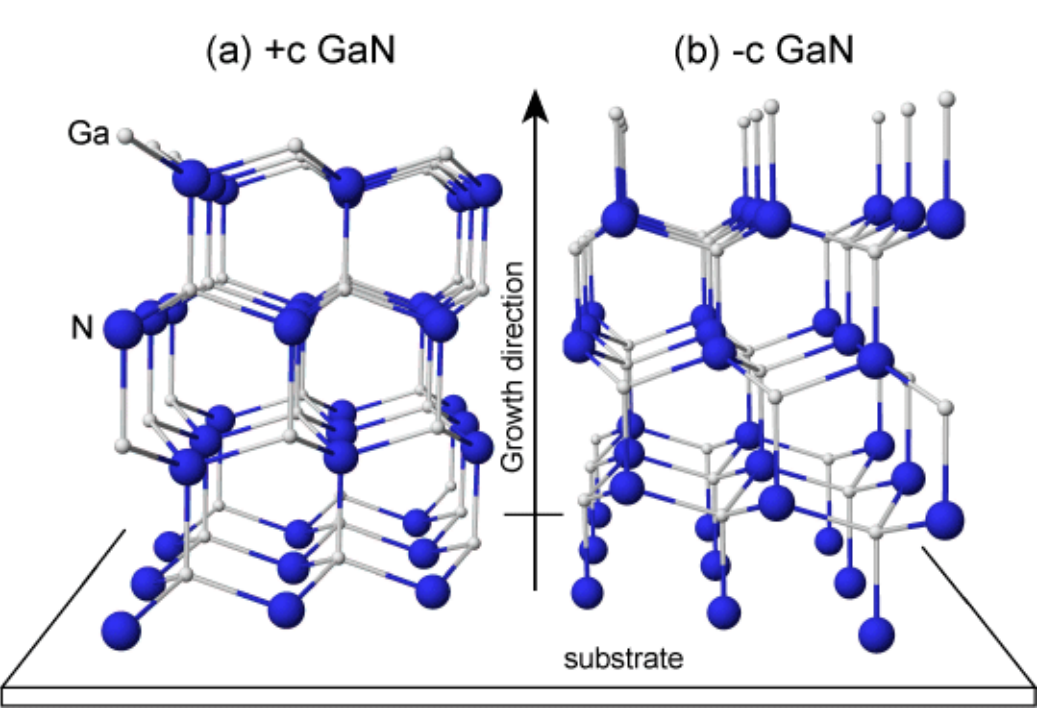
\includegraphics[width=0.5\textwidth]{Figs/Ch1/p2.png}
	\caption {Illustration of Ga-face (+ {\it c}) and N-face (-{\it c}) GaN wrutzite crystal exhibiting polarity along the {\it c}-axis \cite{Sumiya2004}.}
	\label{1.3}
\end{figure}
\FloatBarrier

This non-zero dipole moment is particularly strong for III-nitrides relative to other III-V semiconductors due to the strong electronegativity and small size of nitrogen compared to other group V elements, resulting in a metal-nitrogen bond with greater ionicity than other III-V bonds \cite{wood2007polarization}. Fig.\ref{1.4} shows a GaN unit cell with lattice parameters {\textbf {\it c}} and \textbf{\it a} denoted.

\begin{figure}[h]
	\centering
	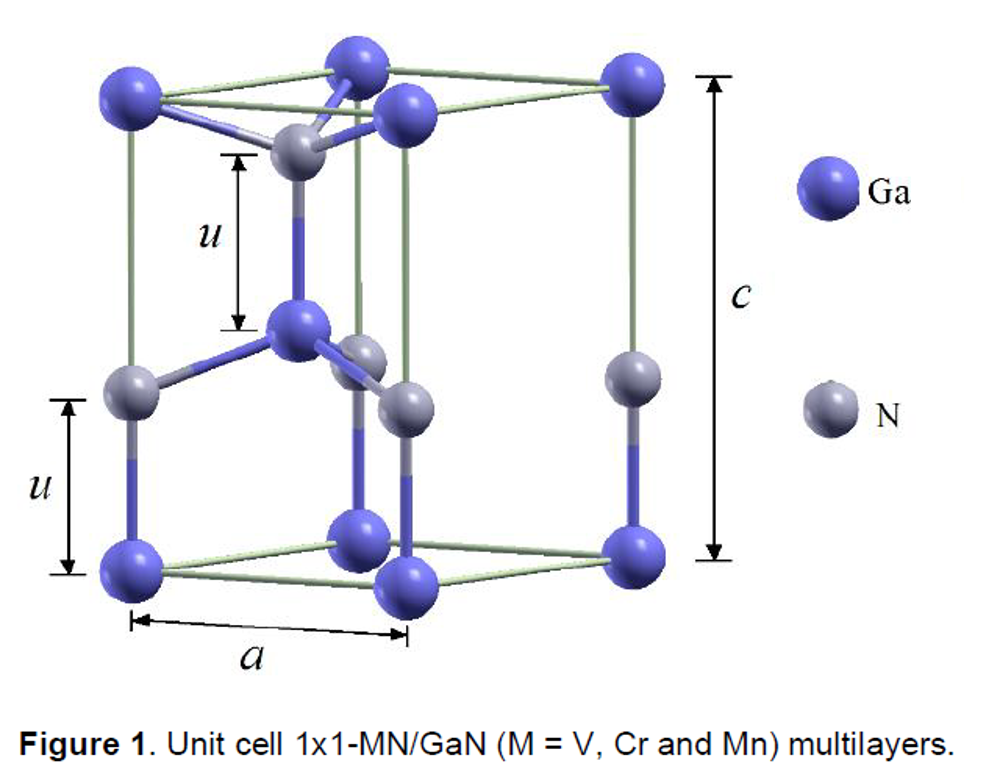
\includegraphics[width=0.5\textwidth]{Figs/Ch1/2unit.png}
	\caption {GaN unit cell with lattice parameters \textbf{\it c} and \textbf{\it a} \cite{Miguel2014}}
	\label{1.4}
\end{figure}
\FloatBarrier 

If all nearest neighbour bond lengths are equal, an ideal hexagonal closed packed crystal exhibiting zero spontaneous polarisation would have a ratio of lattice parameters denoted by:

\begin{equation}
\frac{c}{a}= (\frac{8}{3})^{0.5} = 1.63299
\end{equation} 

The degree of spontaneous polarisation observed in III-nitride materials is thus determined by the amount their lattice parameter ratio deviates from this ideal value. The values for bulk III-nitride materials are given in Table.\ref{tab1.3}. 

\begin{table}[!htb]
	\centering
	\label{tab1.1}
	\begin{tabular}{cc}
		\textbf{Alloy} &  $\mathbf{\frac{c}{a}}$ \\
		%heading
		\hline\hline\\
		GaN   & 1.6259      \\
		InN   & 1.6116     \\
		AlN   & 1.6010   \\ 
		\hline
	\end{tabular}
	\caption{Bulk $\frac{c}{a}$ ratios for GaN, InN and AlN \cite{Ren2015}.}
	\label{tab1.3}
\end{table}

A lower $\mathbf{\frac{c}{a}}$ ratio indicates a higher angle between the three bonds at the base of the tetrahedral bonding structure, resulting in a lower compensation polarisation along the (0001) axis and a higher spontaneous polarisation. Thus according to Table.\ref{tab1.2} the strongest spontaneous polarisation is observed in AlN and the weakest in GaN.\\
It is important to note that materials which exhibit spontaneous polarisation also exhibit piezoelectric polarisation \cite{Ambacher2002}. Strain experienced by the material results in the distortion in of the crystal lattice, which can either alleviate or exacerbate the deviation from the ideal tetrahedral structure resulting in an additional polarisation. This piezoelectric polarization is a crucial consideration in III-nitride devices which often consist of QW heterostructures: lattice mismatches with underlying layers result in the expansion or contraction of III-nitride films. Interestingly two different polarisation configurations are obtained for AlGaN and InGaN coherently strained to GaN. In the case of InGaN the piezoelectric field acts against the spontaneous field, whilst the opposite is true for AlGaN strained to GaN. Within the context of visible light LEDs, InGaN containing QWs are dominated by the piezoelectric contribution to the polarization fields \cite{Fiorentini1999} due to the sizeable lattice mismatch between GaN and InN ($~11\%$) \cite{Chichibu2006}.

\subsubsection{The Quantum Confined Stark Effect}

As previously discussed, III-nitride photonic devices often make use of heterostructures known as quantum wells, which enhance radiative efficiency by confining carrier wavefunctions over a range of several nanometres. Given the presence of built-in fields in III-nitride materials, it is important to consider the effect polarisation fields will have on the band structure and thus optical properties of quantum wells as shown in Fig.\ref{1.5}

\begin{figure}[h]
	\centering
	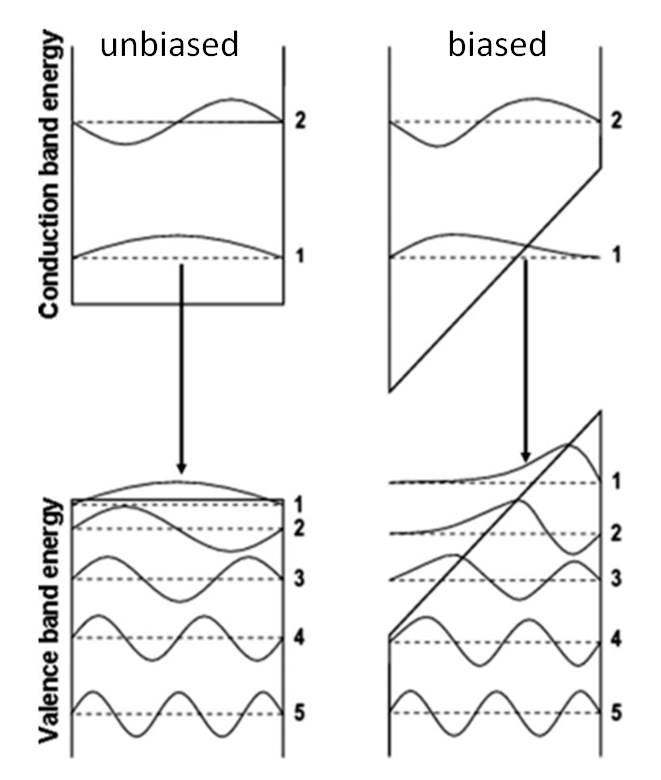
\includegraphics[width=0.5\textwidth]{Figs/Ch1/QCSE.png}
	\caption {Unbiased and biased quantum well energy levels with associated carrier wavefunctions. Under an applied field the overlap between the electron and hole carrier wavefunctions is reduced \cite{Ryou2009}.}
	\label{1.5}
\end{figure}
\FloatBarrier 

The transition from a rectangular to a 'sawtooth'-shaped potential well results in the reduction in energy of the optical transition, meaning the photons emitted from the QW are red-shifted. However, as the carrier density within the QW is increased, by either optical or electrical injection, the polarization fields are effectively screened resulting in a carrier density-dependent optical transition energy.\\
A further effect of the polarization fields is to spatially separate the carrier wave functions, thus reducing their overlap as shown in Fig.\ref{1.5}. This results in a reduced probability for the radiative recombination carriers thus reducing the efficiency of III-nitride QW emitters.
\subsection{Defects in III-nitrides}  %Section - 1.4 
\label{section1.1.4}
Many issues with III-nitride based optoelectronic devices arise from the high defect densities present. Dislocation densities tend to be several orders of magnitude higher for nitride devices relative to other III-V materials due to the lack of a low cost, widely-available lattice matched substrate \cite{Bennett2010b}. Lattice mismatch and alloy-dependent growth temperatures results in the presence of imperfections in the crystal structure of the epitaxial film known as defects. These defects can result in perturbations to the electrical and optical properties of an 'ideal' crystal, and are often classified based on their spatial dimensions. 0-D defects are often referred to as point defects, 1-D defects are commonly termed linear defects or dislocations, 2-D defects are known as planar defects or stacking faults, and there are a variety of 3-D defects known as volume defects.

\subsubsection{0-D Defects}
Point defects exist in four main forms, shown in Fig.\ref{1.6}. Vacancies, where an atom is missing from the lattice, and self-interstitial point defects are termed 'native defects': there is no inclusion of foreign atoms. These two types of intrinsic point defects are shown in Fig.\ref{1.6} a) and b) respectively.\\ 
In the case of GaN, three types of vacancies can exist: gallium vacancies, nitrogen vacancies and divacancies. The gallium vacancy ($V_{Ga}$) which has a low formation energy in {\it n}-type GaN and is acceptor-like, this vacancy has a low migration barrier. Due to this low migration energy, it is expected that gallium vacancies form complexes with more stable defects. Gallium vacancies and associated complexes are thought to be the cause of yellow luminescence observed in {\it n}-type GaN. Nitrogen vacancies initially attracted a large amount of interest due to the common belief that their energy levels were close to or within the conduction band. Due to this, the {\it n}-type conductivity of undoped GaN was attributed to nitrogen vacancies.  However, calculations have shown the thermal equilibrium of nitrogen vacancies to be too low to account for the observed conductivity. Nitrogen vacancies are also expected to have relatively low migration barriers, indicating complexes involving more stable defects may occur during high-temperature growth or annealing, especially in {\it p}-type GaN \cite{Reshchikov2005}. Divacancies have high formation energy in GaN and are not expected to form in large concentrations \cite{Reshchikov2005}.
\\The inclusion of foreign atoms can result in a foreign interstitial point defect, or a substitional impurity, both are shown in Fig.\ref{1.6} c) and d) respectively. The formation of self-interstitial or antisite (swapping of Ga and N lattice positions in the lattice) have a low occurence due to the small lattice constant of GaN and large size mismatch between Ga and N atoms \cite{Reshchikov2005}.
\begin{figure}[t!]
	\centering
	\begin{subfigure}[t]{0.3\textwidth}
		\centering
		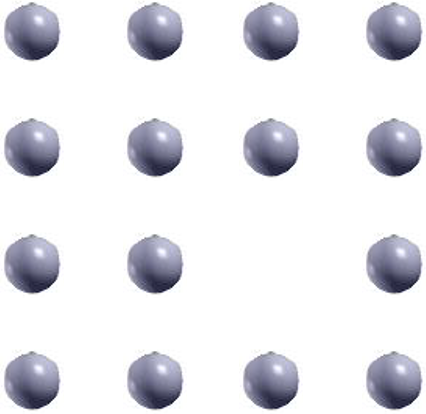
\includegraphics[height=1.2in]{Figs/Ch1/vacancy.png}
		\caption{Vacancy}
		\vspace*{1cm}
	\end{subfigure}%
	~ 
	\begin{subfigure}[t]{0.3\textwidth}
		\centering
		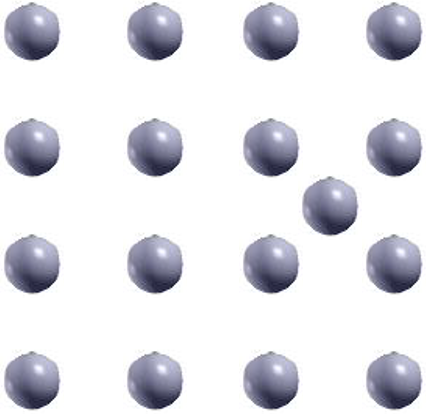
\includegraphics[height=1.2in]{Figs/Ch1/self-inter.png}
		\caption{Self-Interstitial}
	\end{subfigure}
	
	\begin{subfigure}[b]{0.3\textwidth}
		\centering
		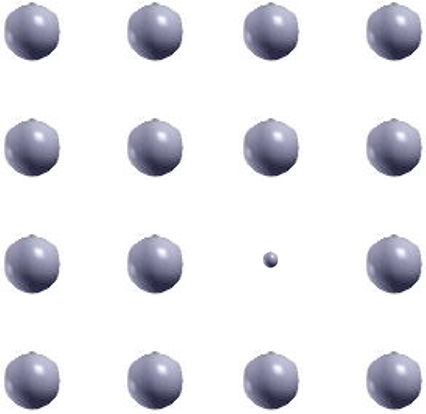
\includegraphics[height=1.2in]{Figs/Ch1/sub-impure.png}
		\caption{Substitutional Impurity}
	\end{subfigure}%
	~ 
	\begin{subfigure}[b]{0.3\textwidth}
		\centering
		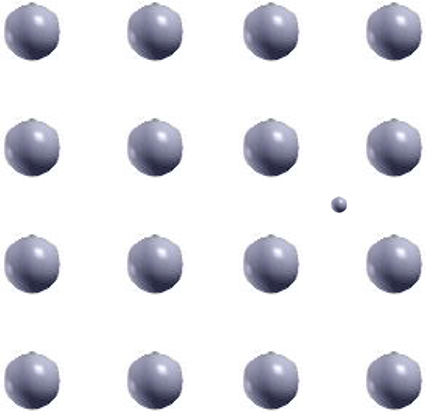
\includegraphics[height=1.2in]{Figs/Ch1/foreign.png}
		\caption{Foreign Interstitial}
	\end{subfigure}
	\caption{Point Defects:vacancy, self-interdtitial, substitutional impurity and foreign interstitial.}
	\label{1.6}
\end{figure}
\FloatBarrier
 Point defects are responsible for a plethora of deleterious effects at the device level in III-nitrides: they can reduce radiative efficiency, produce undesired luminescence act and as parasitic current paths \cite{Reshchikov2005}.
\subsubsection{1-D Defects}
Dislocations in GaN epilayers are categorised in two main forms: misfit dislocations (MDs) and threading dislocations (TDs). The origins of misfit dislocations are quite well understood: they occur through the release of misfit strain at interfaces between two crystals of differing lattice constants. The process is shown in Fig.\ref{1.7}: a film with a lattice parameter greater than the substrate is grown as is typical for III-nitride epilayers (GaN on sapphire or InGaN on GaN) and as a result the grown layer experiences compressive stress and forms pseudomorphic layer. The top layer is strained and matched to the lower layer due to its smaller lattice parameter. Strain relaxation occurs as the pseudomorphic relationship is broken when the top film reaches a critical thickness and results in the formation of misfit dislocations.

\begin{figure}
	\begin{subfigure}[b]{0.3\textwidth}
		\centering
		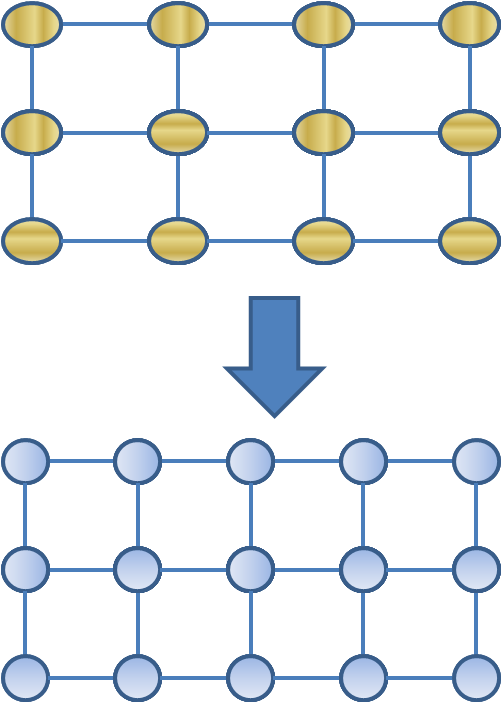
\includegraphics[width=.85\linewidth]{Figs/Ch1/MDa}
		\caption{}
	
	\end{subfigure}%
	\hspace*{0.5cm}
	\begin{subfigure}[b]{0.3\textwidth}
		\centering
		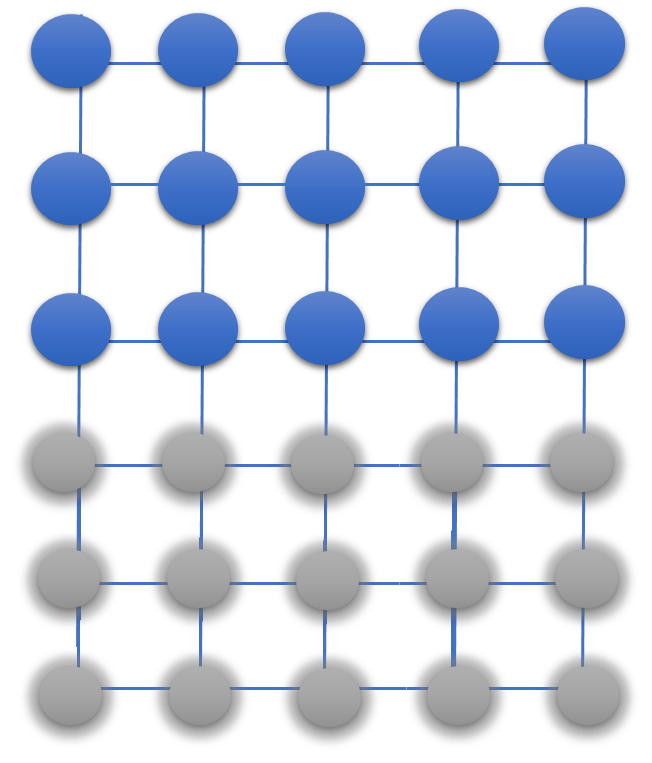
\includegraphics[width=.85\linewidth]{Figs/Ch1/MDb}
		\caption{}
		
	\end{subfigure}%
	\hspace*{0.5cm}
	\begin{subfigure}[b]{0.3\textwidth}
		\centering
		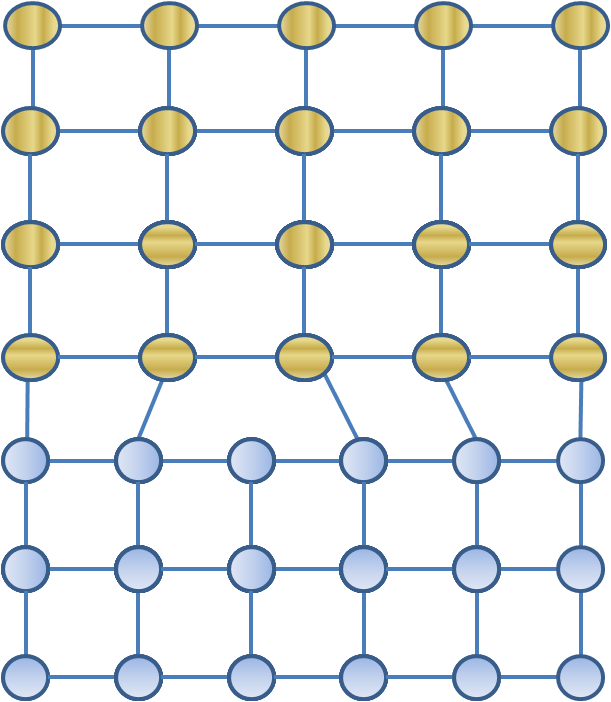
\includegraphics[width=.85\linewidth]{Figs/Ch1/MDc}
		\caption{}
	\end{subfigure}%

	\caption{Misfit dislocation formation through strain relaxation for heteroepitaxial growth: a) the film is grown on a substrate of smaller lattice size b) film maintains a pseudomorphic relationship with the substrate c) the film relaxes through the formation of a dislocation.}
\end{figure}
\FloatBarrier

The origins of TDs are far less well understood. TDs are not believed to relieve mismatch stress, and typically propagate perpendicular to the planar surface. TDs are classified into three categories based on their Burgers vector, as shown in Table.\ref{tab1.4}.

\begin{table}[h]
	\centering
	\begin{tabular}{p{4cm} p{4cm}   }
		\centering
		\textbf{Dislocation type}& \textbf{Burgers vector} \\
		\hline
		$\mathbf{a}$ type & $\frac{1}{3}<11\bar{2}0>$ \\
		$\mathbf{c}$ type& $<0001>$ \\
		$\mathbf{a+c}$ type & $\frac{1}{3}<11\bar{2}3>$ \\
		\hline
		
	\end{tabular}
	\caption{Burgers vectors for pure edge ($\mathbf{a}$), pure screw ($\mathbf{c}$) and mixed ($\mathbf{a+c}$)  TDs}
	\label{tab1.4}
\end{table}
\FloatBarrier

It was initially reported that GaN islands on sapphire during the initial stages of growth may be misorientated with respect to one another and that during the coalescence of these misorientated islands \cite{Ning1996}. This was seemingly disproven by a transmission electron microscopy data from a study on partially coalesced GaN on sapphire layers at various growth stages, which indicated the large majority of TDs seemed to initiate from within the nucleation layers at the GaN/sapphire interface rather than at coalescence boundaries. Oliver {\it et al}. used silane treatment to enlarge dislocation pits and observe them using atomic force microscopy, finding no significant relationship between boundary regions and the locations of dislocations \cite{Oliver2008a}. It was however suggested that dislocations may arise from the overgrowth of smaller islands by larger ones. Thus, while there is convincing evidence that TDs do not originate due to island coalescence, the actual mechanism behind their generation remains poorly understood.

\subsubsection{2-D Defects}

Stacking faults are defects which disrupt the regular stacking sequence of the crystal structure, in non-polar heterostructures they can intersect the QW layers. As a result of this, stacking faults are a more pressing concern than dislocations in epitaxial films grown along alternative directions to the {\it c}
-plane, as in polar materials stacking faults tend to remain in the nucleation layers \cite{Scholz2012}. Fig.\ref{1.7} shows different forms of stacking faults in $(11\bar{2}0)$ GaN ({\it a}-plane) on {\it r}-plane sapphire.  Basal-plane stacking faults \nomenclature[z-BSF]{BSF}{Basal-plane Stacking Fault} (BSFs) are atomic layers with a modified stacking sequence in the wurtzite crystal matrix. These BSFs can transfer to another stacking plane through prismatic stacking faults \nomenclature[z-PSF]{PSF}{Prismatic Stacking Fault} (PSFs). BSFs can also be bound by partial dislocations \nomenclature[z-PD]{PD}{Partial Dislocation} (PDs).


\begin{figure}[h]
	\begin{subfigure}[t]{0.4\textwidth}
	\centering
	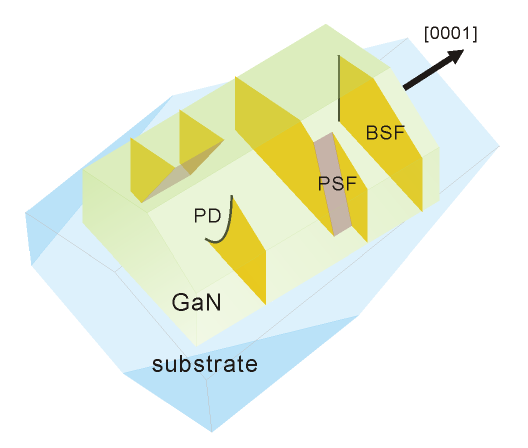
\includegraphics[width = 1\textwidth]{Figs/Ch1/bsf.png}
	\caption{}
	\end{subfigure}%
		\hspace*{1cm}
	~	
	\begin{subfigure}[t]{0.4\textwidth}
		\centering
		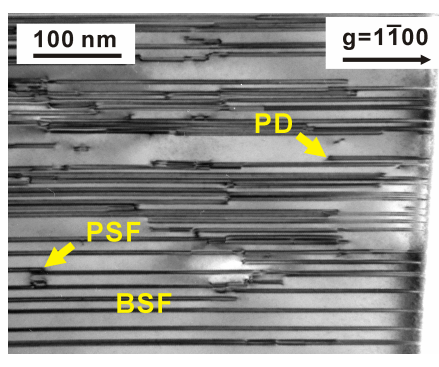
\includegraphics[width=1\textwidth]{Figs/Ch1/bsfTEM.png}
		\caption{}
	\end{subfigure}
	\caption {a) {\it a}-plane GaN showing basal plane stacking faults (BSFs), prismatic stacking faults (PSFs) and stacking faults bounded partial dislocations (PDs) shown schematically b) and in TEM. Adapted from \cite{Liu2011}.}
	\label{1.7}
\end{figure}
\FloatBarrier

Three types of BSFs exist in wurtzite crystals, they are classified based on their displacement vector $\mathbf{\vv{R}}$ as shown in Table.\ref{tab1.5}.

\begin{table}[h]
	\centering
	\begin{tabular}{cc}
		\centering
		\textbf{BSF type}& \textbf{Displacement vector $\mathbf{\vv{R}}$ } \\
		\hline
		$I_{1}$  & $\frac{1}{6}<20\bar{2}3>$ \\
		$I_{2}$ & $\frac{1}{3}<10\bar{1}0>$ \\
		$E$  & $\frac{1}{2}<0001>$ \\
		\hline
		
	\end{tabular}
	\caption{BSF types in wurtzite materials.}
	\label{tab1.5}
\end{table}
\FloatBarrier

Whilst TDs are considered completely undesirable due to the adverse effects they may have on radiative processes and carrier transport, it has been suggested the presence of BSFs on the optical properties may be beneficial in some cases. Indeed, BSFs have been shown to enable radiative recombination through confinement and thus act as QWs with an exciton binding energy of 45 meV \cite{Rebane1997}.

\subsubsection{3-D Defects}

There are many forms of 3-D defects in III-nitrides such as voids, nanopipes and cracks. In this particlar section we will focus on those relevant to the work featured in later chapters of this work.\\
Inverted hexagonal pyramid defects, also known as V-pits, are defects commonly found at the surface of InGaN/GaN QW structures. They form as a result of a TD intersecting the QW layers. It is believed that the low temperatures required for the growth of the InGaN layers allow even minute perturbations of the surface to persist into inclined facets with low growth rates, such as the $(1\bar{1}01)$ facets. The apex of TDs thus provide optimal conditions for the formation of V-pits during the growth of InGaN layers \cite{Hangleiter2005}. Interestingly, TEM studies have shown that the QW layers disrupted by the defect grow along the semi-polar facets at a lower thickness \cite{Hangleiter2005,Han2013,Tsai2007}. Fig.\ref{1.8} shows a TEM image of a V-pit in an InGaN/GaN multiple QW structure with a schematic describing this defect and how it affects the growth of the QWs.

\begin{figure}[h]
	\centering
	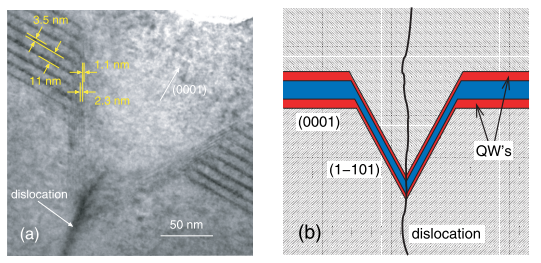
\includegraphics[width=0.7\textwidth]{Figs/Ch1/vpit.png}
	\caption {a) TEM image of a hexagonal inverted pyramid defect b) Schematic  of a V-pit with its associated TD \cite{Hangleiter2005}.}
	\label{1.8}
\end{figure}
\FloatBarrier 

The existence of TDs as non-radiative recombination centres has been well documented \cite{Bennett2010b}, however it is believed that V-pits suppress this non-radiative recombination and provide an increase in light emission efficiency in III-nitride devices by providing an energy barrier surround TDs \cite{Hangleiter2005}. Hangleiter {\it et al}. suggested the thinner wells grown along the semi-polar facets of the V-pit provided an energy barrier of several hundred meV relative to the normal {\it c}-plane QWs \cite{Hangleiter2005}, thus providing a potential landscape shielding carriers from TDs, as shown in Fig.\ref{1.9}.

\begin{figure}[h]
	\centering
	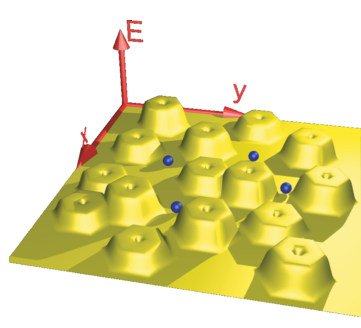
\includegraphics[width=0.5\textwidth]{Figs/Ch1/landscape.png}
	\caption {Potential landscape due to V-pits decorating the apex of TDs: carriers (blue) need to overcome the energy barriers to recombine non-radiatively at the TDs \cite{Hangleiter2005}.}
	\label{1.9}
\end{figure}
\FloatBarrier 

 
%********************************** %Second Section  **************************************
\section{III-nitride Devices } %Section - 1.1 
\subsection{Light Emitting Diodes}
Light emitting diodes (LEDs) are the most common application of III-nitride materials. These devices typically consist of a {p-n} junction. This consists of material containing excess acceptor ({\it p}-doped) and another containing excess donor impurities ({\it n}-doped) which are brought into contact. This allows holes from the {\it p}-type material and electrons from the {\it n}-type material to diffuse across the junction until an equilibrium state is reached, a region where the electric field from the charged dopants on either side prevents diffusion is formed known as the depletion region. The application of forward bias reduces the built-in potential across the depletion region and allows for the flow of electrons and holes across the junction, as shown schematically in Fig.\ref{1.10}.
\begin{figure}[h]
		\hspace*{1cm}
	\begin{subfigure}[t]{0.4\textwidth}
		\centering
		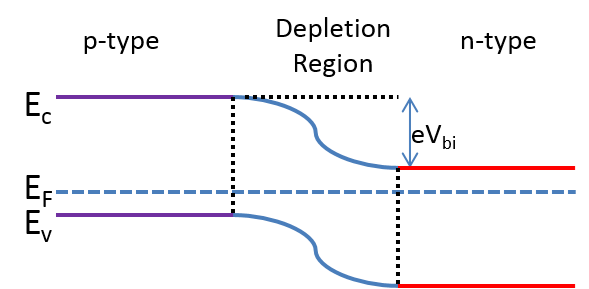
\includegraphics[width = 1\textwidth]{Figs/Ch1/pn1.png}
		\caption{}
	\end{subfigure}%
	\hspace*{1cm}
	~	
	\begin{subfigure}[t]{0.4\textwidth}
		\centering
		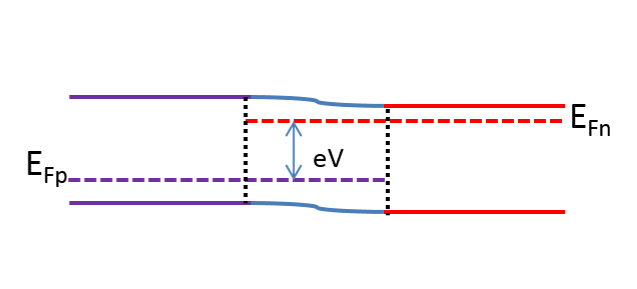
\includegraphics[width=1\textwidth]{Figs/Ch1/pn2.png}
		\caption{}
	\end{subfigure}
	\caption {a) {\it p-n} junction at equilibrium, with the conduction band, Fermi level and valence band denoted $E_{c},E_{F}$ and $E_{v}$ respectively, the built in potential across the junction is denoted as $V_{bi}$ b) under forward bias of V.}
	\label{1.10}
\end{figure}
\FloatBarrier

A schematic of a general LED structure is shown in Fig.\ref{1.11}. Visible light LED structures typically contain a magnesium doped {\it p}-region and a silicon doped {\it n}-region. An electron blocking layer \nomenclature[z-EBL]{EBL}{Electron Blocking Layer} (EBL) consisting of a material with a higher bandgap than GaN ( in this case AlGaN) is used to prevent the leakage of electrons into the {\it p}-doped region and confine them in the InGaN QW active region.

\begin{figure}[h]
	\centering
	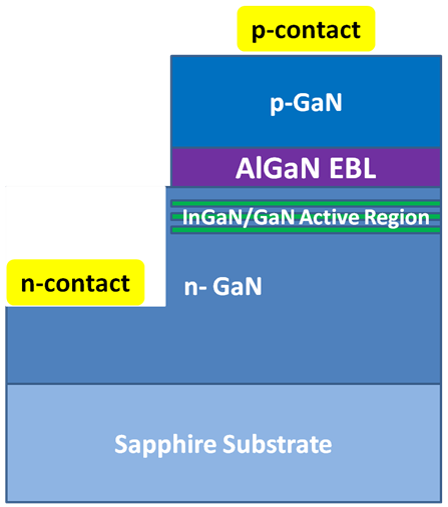
\includegraphics[width=0.3\textwidth]{Figs/Ch1/led.png}
	\caption {Typical visible light LED structure grown on a sapphire substrate \cite{Ren2015}.}
	\label{1.11}
\end{figure}
\FloatBarrier 

\subsection{Microcavities}

Microcavity emitters possess rather singular optical properties due to their dimensions. By matching one or more dimensions of the cavity to the order of the wavelength of confined light a plethora of effects can be produced such as low-threshold lasing, directional luminescence and enhanced nonlinear conversion \cite{Christopoulos2007}. By confining a dipole within a microcavity, one can modify its emissive properties by altering the photon density of states. The interaction rate between the confined dipole and a cavity photon relative to the average rate of dissipation of a cavity determines whether the microcavity operates in the weak-coupling or strong-coupling regime.\\Weak coupling occurs when dissipation overwhelms the dipole-cavity photon interaction: in essence, the effect of the microcavity in this case is to alter the vacuum description of the dipole lifetime, resulting in an increase in spontaneous emission for on-resonance cavity modes, known as the Purcell effect \cite{Vahala2003}. Weakly-coupled microcavity systems have applications across a wide range of optoelectronic devices due to this effect: from enhancing the recombination rate and extraction efficiency of embedded single photon emitters \cite{Jarjour2007a} to the development of high efficiency, low threshold lasers \cite{Aharonovich2013}.\\An interaction occurring on shorter timescales than the average dissipation rate of the cavity photon is defined as being in the strong coupling regime, and results in the formation of admixed eigenstates populated by quasiparticles known as polaritons, which are hybrid particles combining a photon and an electric dipole. The bosonic nature of these quasiparticles has led to the observation of spontaneously emitted coherent light from condensates of exciton-polaritons,  a phenomenon also known as polariton lasing \cite{Malpuech2002}. The expected threshold energy for coherent emission from a polariton laser is expected to be much smaller than that of a conventional laser due to the lack of the requirement of population inversion , thus rendering polariton lasers extremely attractive as low-threshold lasing applications \cite{Christopoulos2007}. Beyond polariton lasing, strong coupling in microcavities is also required for key quantum information processing tasks such as the entanglement of distinguishable quantum systems and controlled coherent coupling \cite{Imamoglu1999,Hennessy2007}.

\subsubsection{Cavity Parameters and Design}
The ability of a microcavity to confine light is thus a crucial parameter in producing the required effects and is known as the cavity 'quality factor' which is described by Eq.~\ref{Q-fac}.

\begin{equation}\label{Q-fac}
Q = \frac{\nu_{0}}{\delta\nu_{0}}
\end{equation}

Where $\nu_{0}$ is the resonant frequency of the cavity mode and $\delta\nu_{0}$ is the mode bandwidth. Cavity quality factor can be understood as a parameter describing the rate of energy decay the resonant mode undergoes within the cavity and thus may be alternatively described using an exponential characteristic decay constant $\tau_{cav}$ as shown in Eq.\ref{exp}, where $Q^{-1}$ is the proportion of energy lost during a single cavity round-trip.

\begin{equation}\label{exp}
Q = \pi\tau_{cav} \nu_{0}
\end{equation}

The manner in which the resonant mode fields interact with the cavity geometry is also determined by the effective modal volume of the cavity, which is described by Eq.\ref{mode}.

\begin{equation}\label{mode}
V_{eff}= \int_{V}\frac{\epsilon_{0}(\mathbf{r})|\mathbf{E}(\mathbf{r})|^{2}}{max[\epsilon_{0}(\mathbf{r})|\mathbf{E}(\mathbf{r})|^{2}]}dV
\end{equation}

where $|\mathbf{E}(\mathbf{r})|^{2}$ is the normalised electric field amplitude, $\epsilon_{0}$ is the dielectric constant and V is the quantization volume. $V_{eff}$ describes the manner in which cavity supports the distribution of the resonant mode, thus in some cases a large evanescent field component must be included in the calculation of the modal volume.
\\ Cavities often support more than one optical mode, which gives rise to another parameter, known as the free spectral range \nomenclature[z-FSR]{FSR}{Free Spectral Range} (FSR), which is defined as the frequency spacing between successive resonant modes. This parameter is crucial to lasing cavities as the probability of photon into a lasing mode is affected by the number of modes supported by the cavity. The FSR as well as parameters needed to define cavity quality factor are shown schematically in Fig.\ref{1.12}. 

\begin{figure}[h]
	\centering
	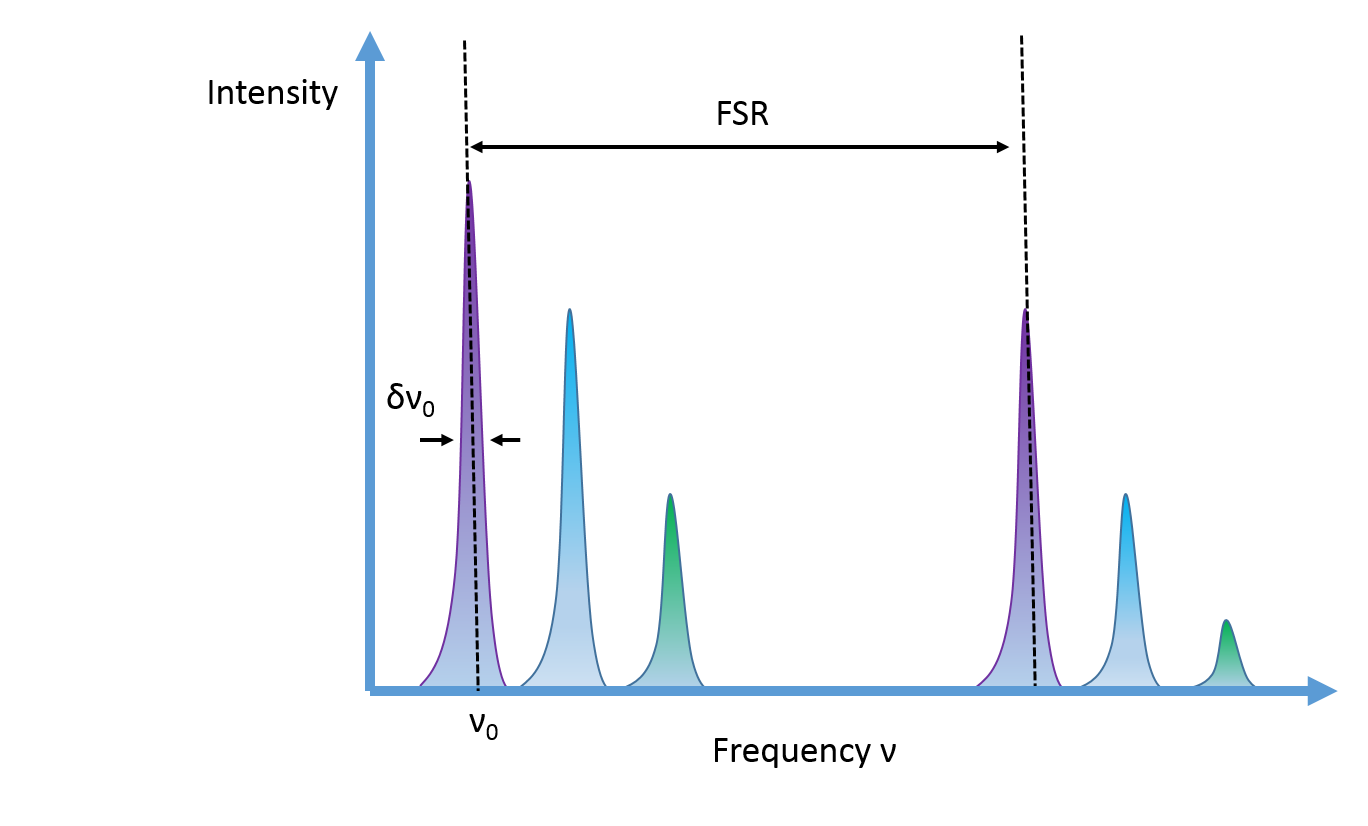
\includegraphics[width=0.9\textwidth]{Figs/Ch1/modes.png}
	\caption {Illustration of the some key parameters such as FSR and resonant cavity mode FWHM. }
	\label{1.12}
\end{figure}
\FloatBarrier 


Cavities modify the optical density of states of an emitter through the generation of standing electromagnetic waves. There are several manners through which to achieve this: at the most basic level an optical cavity is a set of single reflective interfaces, spaced at a specific distance designed to enhance a particular optical mode. However, many cavity designs which employ the use of refractive index mismatches for total internal reflection or an array of boundaries leading to interference enhanced optical modes also exist, as shown in Fig.\ref{1.13}.
\begin{figure}
	\begin{subfigure}[b]{0.3\textwidth}
		\centering
		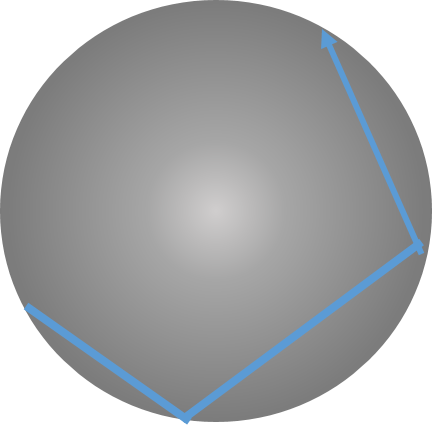
\includegraphics[width=.75\linewidth]{Figs/Ch1/mdisk}
		\caption{Total internal reflection}
		
	\end{subfigure}%
	\hspace*{0.5cm}
	\begin{subfigure}[b]{0.3\textwidth}
		\centering
		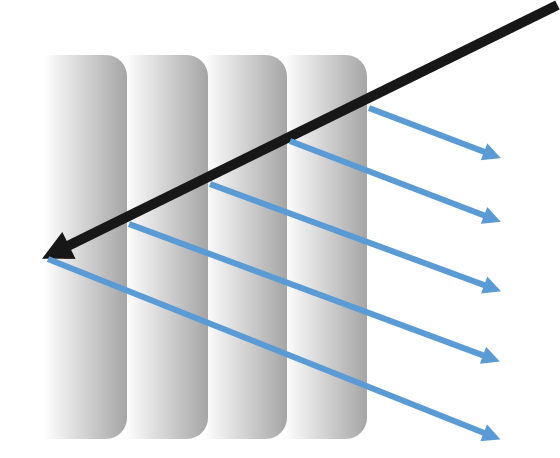
\includegraphics[width=.85\linewidth]{Figs/Ch1/dbr}
		\caption{1-D interference}
		
	\end{subfigure}%
	\hspace*{0.5cm}
	\begin{subfigure}[b]{0.3\textwidth}
		\centering
		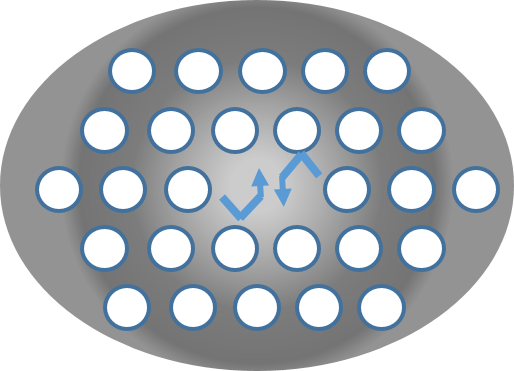
\includegraphics[width=.85\linewidth]{Figs/Ch1/pcc}
		\caption{2-D interference}
	\end{subfigure}%
	
	\caption{Optical resonators.}
	\label{1.13}
\end{figure}

\FloatBarrier

\subsubsection{Microdisk Cavities}

Total internal reflection can be exploited in circular geometries such as microdisk/ring/sphere devices, in which whispering gallery modes \nomenclature[z-WGM]{WGM}{Whispering Gallery Mode} (WGMs) propagate around the periphery of the disk.\\
Microdisks can be described as a cylinder of with a low height:radius ratio supported by a pillar of a small radius ( less than half of the cylinder). The position of the WGMs is described by Snell's law: only light satisfying the condition described by Eq.\ref{eq1} is contained within the microdisk due to internal reflection.

\begin{equation} \label{eq1}
\theta_{c}=sin^{-1}(\frac{n_{2}}{n_{1}})
\end{equation}

Assuming the microdisk thickness is small enough to act as a waveguide in the vertical direction, we can consider the propagation of a ray of light in 2-D as in Fig.\ref{1.14}. The forbidden position of the WGMs as defined by Eq.\ref{eq1} is given by $R_{min}$.
\begin{figure}[h]
	\centering
	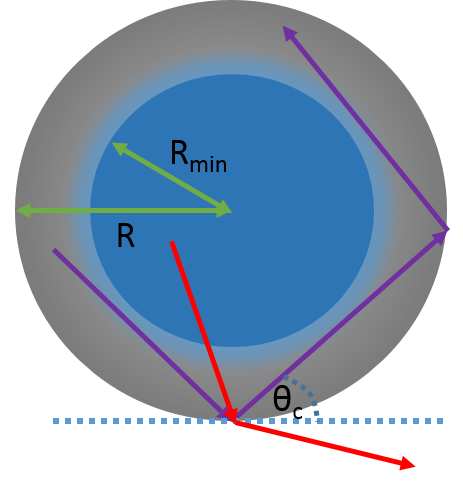
\includegraphics[width=0.5\textwidth]{Figs/Ch1/mdiskray.png}
	\caption {Illustration of the minimum radius $R_{min}$ for WGM propagation. Rays traversing the region $r<R_{min}$ (denoted in red) exceed the critical angle $\theta_{c}$ and thus escape the cavity. Rays travelling outside this region $r>R_{min}$ (denoted in violet) are confined.  }
	\label{1.14}
\end{figure}
\FloatBarrier 
Thus the fabrication of microdisks relies heavily on the ability to 'undercut' the microdisk material whilst still leaving a pedestal, as shown in Fig.\ref{1.15}. This is a particularly difficult problem to address in terms of III-nitride materials due to the excellent thermal ande chemical stability of GaN.  Early efforts in microdisk nitride fabrication involved dry-etching processes, utilising the refractive index mismatch between the light emitting GaN layers and the sapphire substrate to confine light \cite{Tamboli2007}. Although stimulated emission and lasing was observed by Chang {\it et al}. in dry-etched GaN microdisk cavities \cite{Chang1999}, Haberer {\it et al}. \cite{Haberer2004} reduced the required excitation power densities for lasing by an order of magnitude by employing photoelectrochemical (PEC) etching to undercut GaN microdisks, thus providing superior optical confinement due to the index contrast of the GaN/air interface  relative to the GaN/sapphire interface used by Chang {\it et al}. \cite{Chang1999}. Further improvements in fabrication were achieved by Tamboli et al. with room temperature lasing achieved in GaN/InGaN microdisks through enhancements in microdisk circularity and sidewall smoothness \cite{Tamboli2007}. 
\begin{figure}[h]
	\centering
	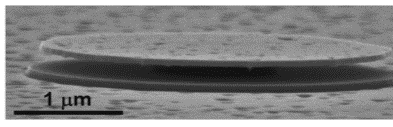
\includegraphics[width=0.5\textwidth]{Figs/Ch1/mdisksem.png}
	\caption {Scanning electron microscope image of a GaN microdisk produced by selective etching of sacrificial AlInN layers \cite{Simeonov2008}.}
	\label{1.15}
\end{figure}
\FloatBarrier 


\subsubsection{Nanobeam Cavities}

Photonic crystals are periodic structures which affect photons in an manner analogous to the way atomic lattices affect electrons in solids. They can be considered as artificial materials exhibiting a dielectric function which varies periodicially in either one, two or three dimensions. The principal mechanism of light confinement in this case is known as distributed bragg reflection as is shown in Fig.\ref{1.13}b).\\
Whilst micro-toroid and microdisk cavities have the potential to achieve extremely high Q-factors many applications which involve strong coupling, non-linear optical processes and spontaneous emission and other similar processes require a high ratio between the Q-factor and the effective modal volume ($V_{eff}$). This figure of merit can be achieved in travelling-wave cavity geometries due to the potential for extremely small modal volumes. Yablonovitch \cite{Yablonovitch1987} and John \cite{John1987} first proposed the design of 3-D photonic crystal cavities which in theory would possess ultra-high Q-factors, minute modal volumes and perfect reflectivity in all directions. Despite the extremely promising theoretical properties of 3-D photonic crystal cavities, their fabrication has proven to be particularly challenging with few demonstrations of high-Q 3-D PCCs reported in literature \cite{Ishizaki2013}, \cite{Tandaechanurat2011}. PCCs of lower dimensionality are thus prime candidates for practical applications due to fewer (though not vanishing!) fabrication issues. In particular 1-D PCCs such as suspended structures known as nanobeams are extremely promising due their ability to realise of high-Q, low $V_{eff}$ cavities even in low index materials such as $SiO_{2}$ \cite{Gong2010}. For these reasons we will specifically be considering 1-D photonic crystal cavities in the nanobeam geometry in this work.\\
Electromagnetic field confinement is achieved in nanobeam structures by Bragg scattering from the photonic crystal in one direction, and index guiding in the other two directions. A nanobeam can essentially be considered as a wavelength-scale Fabry-Perot cavity with photonic crystal mirrors \cite{Deotare2009}: as the nanobeam waveguide mode is trapped and reflected by these mirrors, it also penetrates some distance into them. If the fields terminate at the mirror boundaries, this would lead to large scattering losses due to the large impedance mismatch \cite{Notomi2008}. In order to avoid this impedance mismatch between the waveguide mode and the Bloch mode of the mirror, the photonic crystal mirrors are tapered in order to match the evanescent mirror Bloch mode \cite{Lalanne2003} as shown in Fig.\ref{1.16}.


\begin{figure}[h]
	\centering
	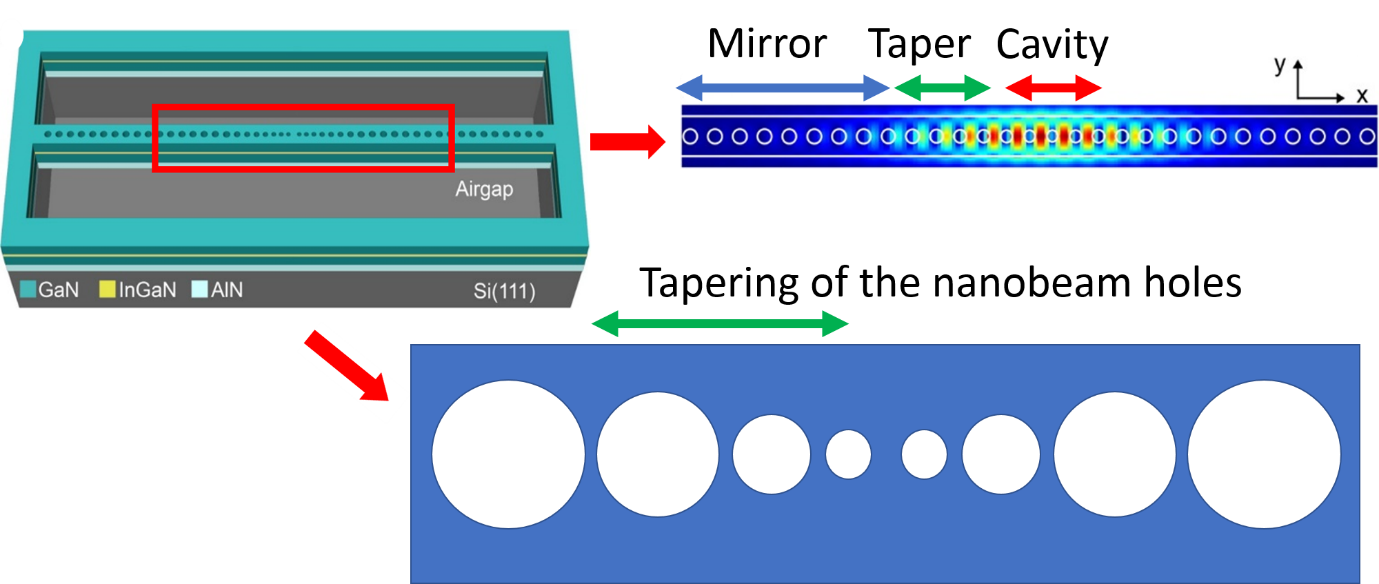
\includegraphics[width=0.9\textwidth]{Figs/Ch1/nb1.png}
	\caption {Nanobeam schematic and 3-D FDTD simulation of the electric field intensity profile of the cavity mode adapted from \cite{Trivino2015}. }
	\label{1.16}
\end{figure}
\FloatBarrier 

\subsection{Nanowires}
The lack of readily available, low-cost substrates for the epitaxial growth of GaN and its associated alloys has motivated research into the growth of III-nitrides in nanowire geometries. Indeed, studies have shown that epitaxial GaN nanowires can be grown with far lower dislocation densities relative to bulk GaN due to a large surface-to-volume ratio. Furthermore, QWs grown radially along the non-polar facets of nanowires allow for the reduction of the polarization fields which can deleteriously affect the optical properties of polar III-nitride emitters without the need for expensive non-polar substrates. Furthermore, axial heterostructure nanowire geometries allow for the growth of {\it p-n} junctions within a single nanowire, allowing for the use of III-nitride nanowires as fundamental electrical components in optoelectronics. As such III-nitride nanowires have been utilised to develop high efficiency LEDs, electrically pump lasers with extremely low lasing thresholds and single photon sources with site-controlled QDs.

\begin{figure}

	\begin{subfigure}[b]{0.49\textwidth}
		\centering
		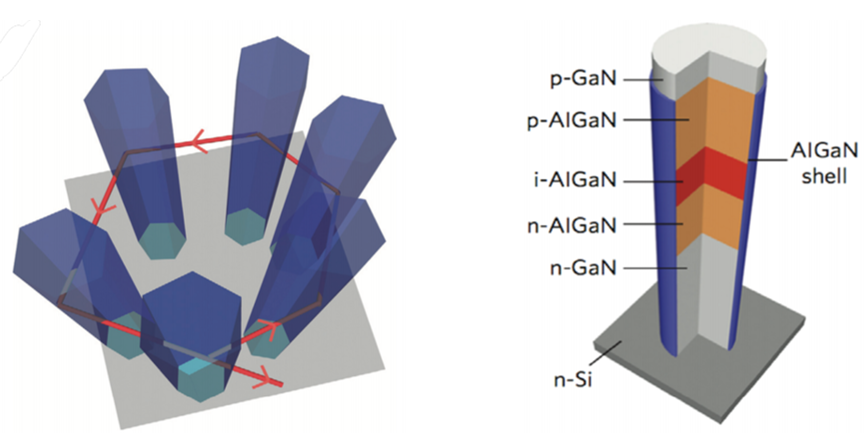
\includegraphics[width=.95\linewidth]{Figs/Ch1/Nwlaser.png}
		\caption{Axial GaN/AlGaN heterostructure nanowire for random lasing\cite{Li2015}}
		
	\end{subfigure}%
	\hspace*{0.5cm}
	\begin{subfigure}[b]{0.49\textwidth}
		\centering
		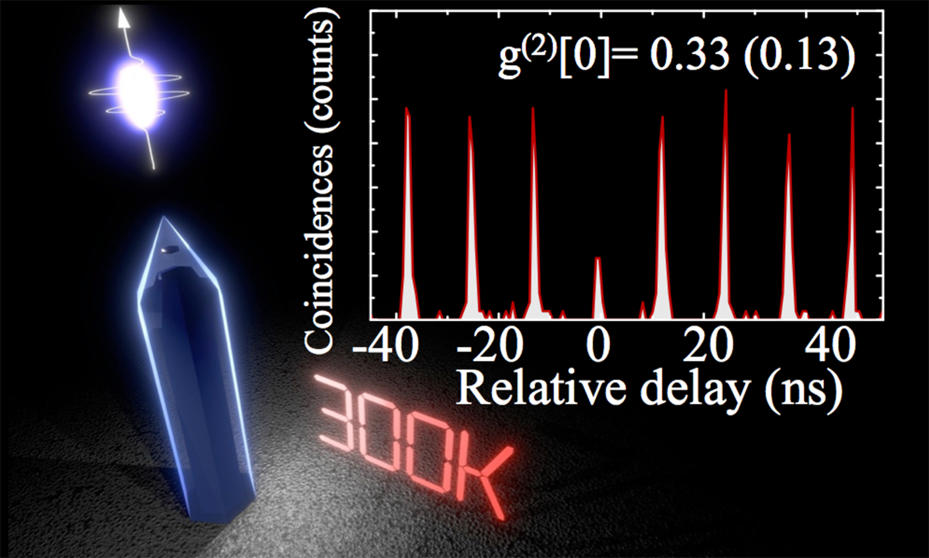
\includegraphics[width=.85\linewidth]{Figs/Ch1/holmes.png}
		\caption{Site-controlled QD in a GaN nanowire showing photon anti-bunching emission at room temperature \cite{Holmes2014}.}
	\end{subfigure}%
	
	\caption{III-Nitride nanowire applications.}
	\label{1.19}
\end{figure}

\FloatBarrier

%*******************************************************************************
%****************************** Second Chapter *********************************
%*******************************************************************************

\chapter{Experimental Methods}

\section{Atomic Force Microscopy}
Atomic force microscopy  \nomenclature[z-AFM]{AFM}{Atomic Force Microscopy} is a non-destructive characterisation technique which employs a sharp tip mounted on a cantilever which is rastered across a sample surface. Tip-surface interactions result in changes cantilever position which are measured using the reflection of laser light reflecting off the cantilever and a four-quadrant photodetector as shown in Fig.\ref{2.1}.

\begin{figure}[h]
	\centering
	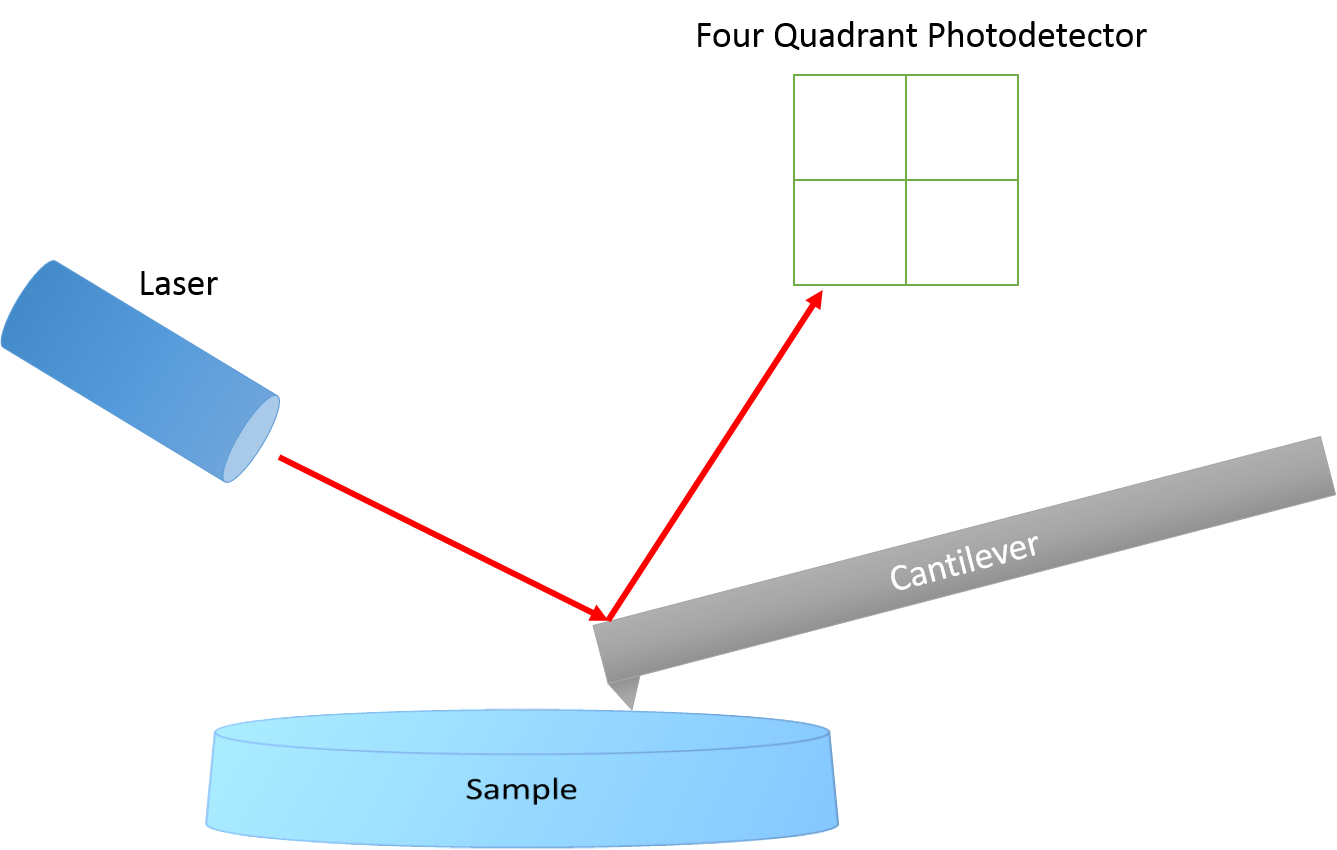
\includegraphics[width=0.7\textwidth]{Figs/Ch2/AFM.png}
	\caption {Schematic of an atomic force microscope.}
	\label{2.1}
\end{figure}
\FloatBarrier

The positioning and movement of the tip is achieved through the use of piezo-electric actuators. In contact mode, a feedback circuit is used to apply a voltage to the piezoelectric crystal in order to maintain a constant tip-sample separation should the tip encounter any features, thus avoiding damage to either the tip of sample. The voltage required to maintain this distance (also known as the setpoint) is registered at each pixel of the scan and is used in conjunction with calibration data to determine a vertical displacement value, thus generating a topographic image.\\
An alternative mode of operation known as tapping mode is often referred to contact mode. In this mode of operation the tip is made to oscillate close to its resonant frequency by the piezocrystal. Contact  between the tip and the sample is achieved at the lowest point of each oscillation, which damps the oscillation of the tip. The oscillation frequency is maintained by the piezoelectric crystal, thus allowing for the generation of a topographic map. Tapping mode is often preferred to contact mode due to the exclusion of lateral friction which can cause tip wear and sample damage.\\
The forces experienced by the tip vary depending on the tip-sample separation, as shown in Fig.\ref{2.2}. Van der Walls forces dominate at large separations attractive the tip to the surface. As the distance is reduced repulsive forces such as hard-sphere repulsion, electron-electron Coulomb interaction and the Pauli-exclusion interaction being to dominate. The sum of these forces result in cantilever deflection, changing the tip-sample interaction.

\begin{figure}[h]
	\centering
	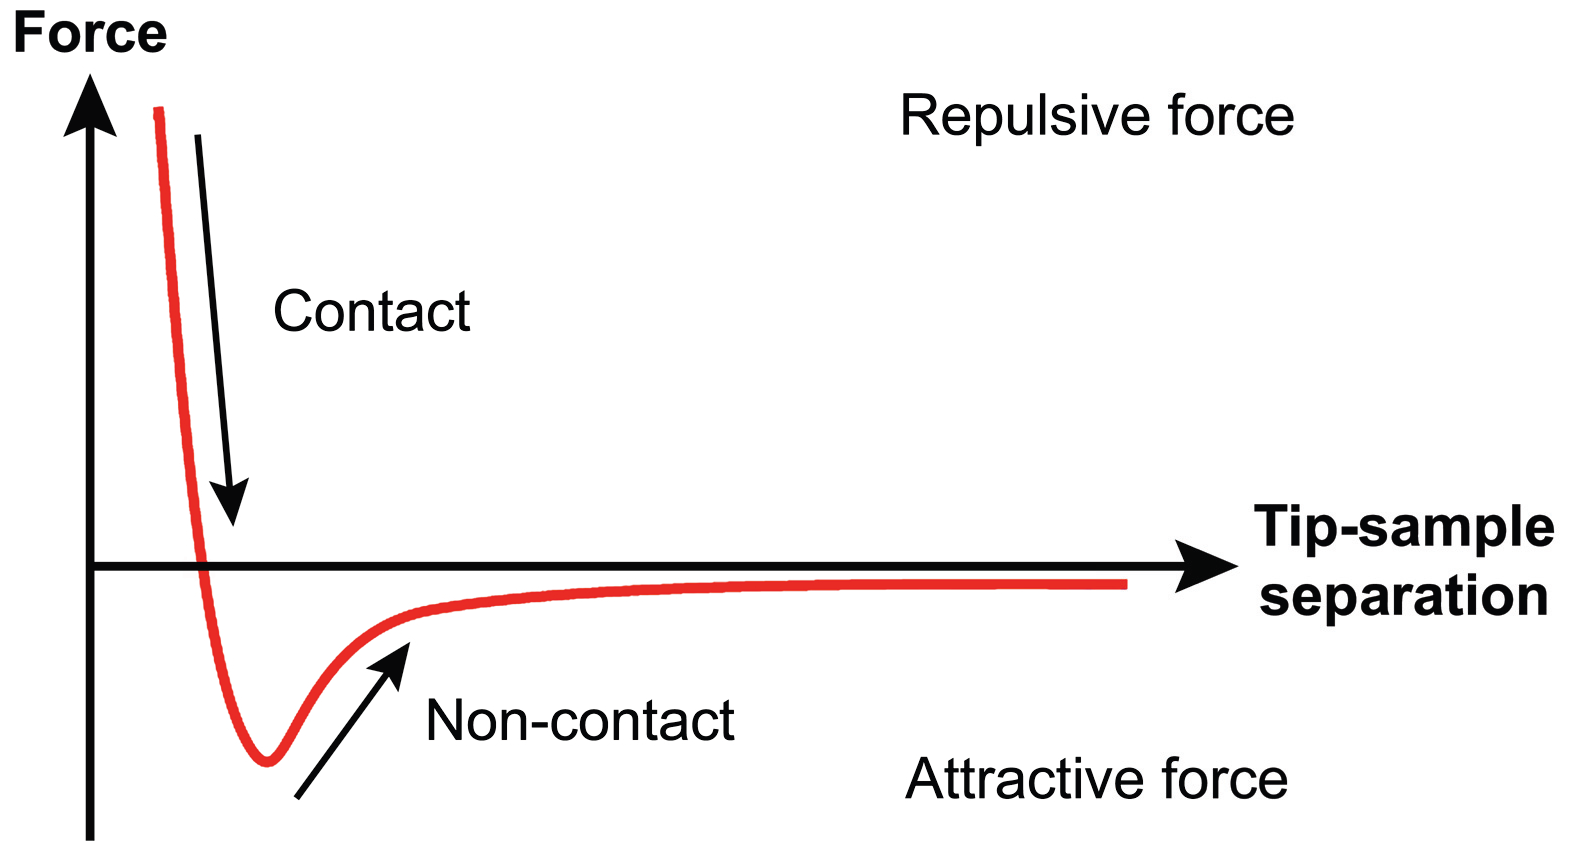
\includegraphics[width=0.7\textwidth]{Figs/Ch2/AFMint.png}
	\caption {The effect of separation on the tip-sample interaction force \cite{Zhu2010}.}
	\label{2.2}
\end{figure}
\FloatBarrier

AFM offers excellent vertical resolution limited only by the probes vertical movement and external noise. However, the lateral resolution of this microscopy technique is heavily dependent on the shape and size of the tip employed. This is perhaps best highlighted by Fig.\ref{2.3} which depicts a hemispherical tip scanning across a flat-topped island. The apex of the tip is in contact with the surface, but the side of the island also experiences some contact: in this case there is a distinction between the two cases shown in Fig.\ref{2.2}a) and b) as the error in the measured width of the island varies based on the relative size of the measured object to the tip.

\begin{figure}[h]
	\begin{subfigure}[t]{0.4\textwidth}
		\centering
		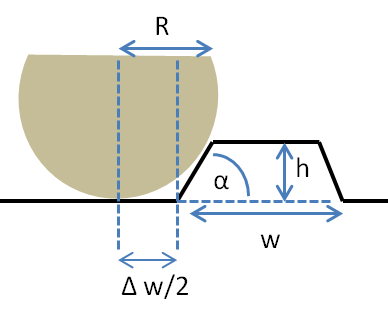
\includegraphics[width = 1\textwidth]{Figs/Ch2/afm1.png}
		\caption{}
	\end{subfigure}%
	\hspace*{1cm}
	~	
	\begin{subfigure}[t]{0.4\textwidth}
		\centering
		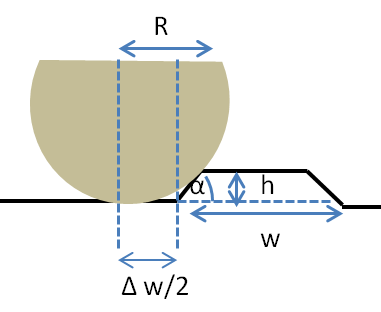
\includegraphics[width=1\textwidth]{Figs/Ch2/afm2.png}
		\caption{}
	\end{subfigure}
	\caption {Interaction of a hemisphere with a flat-topped island for the cases a) $h > R(1-cos(\alpha))$ and b) $h < R(1-cos(\alpha))$ adapted from \cite{Oliver2008}. }
	\label{2.3}
\end{figure}
\FloatBarrier 

Similarly, when measuring depth rather than height the ability of the tip to penetrate into the spaces being measured is also a crucial consideration, as shown in Fig.\ref{2.4}. Thus, increasing the gradient of the tip and minimizing the tip apex are descriable to reduce tip-related measurement artefacts when performing atomic force microscopy.

\begin{figure}[h]
	\centering
	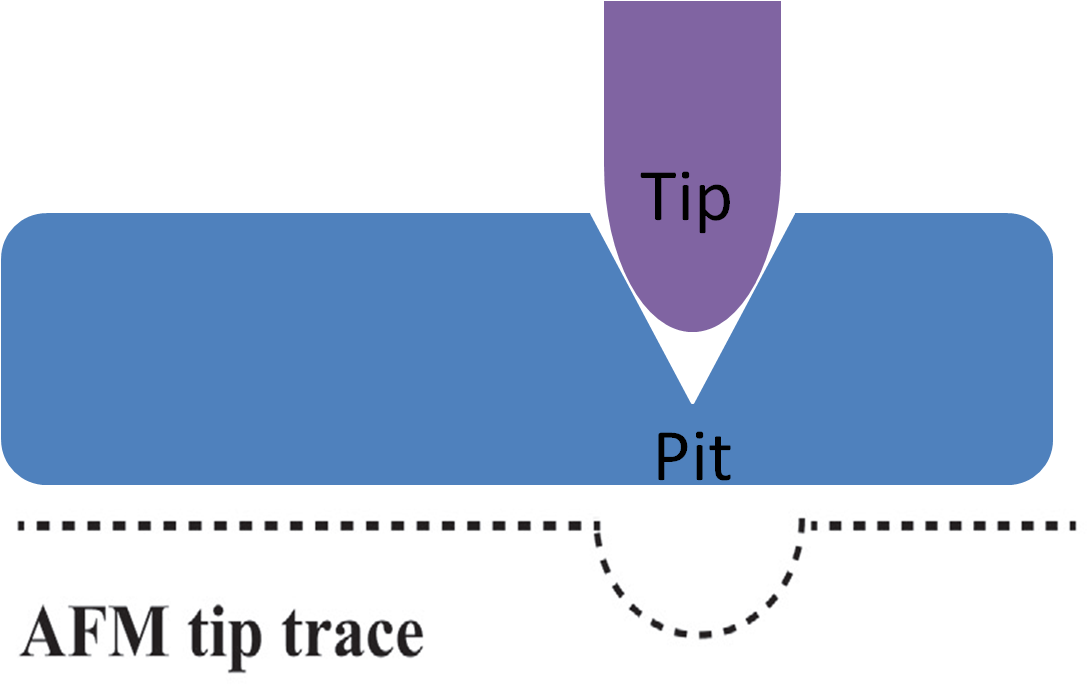
\includegraphics[width=0.4\textwidth]{Figs/Ch2/afm3.png}
	\caption {Measurement error in the depth of a pit caused by the finite width of the AFM tip.}
\end{figure}
\FloatBarrier

\subsubsection{Conductive Atomic Force Microcsopy}

Conductive atomic force microscopy \nomenclature[z-C-AFM]{C-AFM}{Conductive Atomic Force Microscopy} is a technique which combines AFM with local conductivity measurements. In order to perform C-AFM a conductive probe tip is brought close to contact with the sample and a bias is applied between the tip and the sample. The short tip-sample separation causes electron wavefunctions in the tip and sample to overlap, thus allowing a tunneling current to be generated through the application of a bias. C-AFM thus allows for the simultaneous measurement of tip-sample current flow and surface morphology, making it an extremely powerful tool to probe local sample conductivity. 


% Uncomment this line, when you have siunitx package loaded.
%The SI Units for dynamic viscosity is \si{\newton\second\per\metre\squared}.


\section{Scanning Electron Microscopy Techniques}

A scanning electron microscope  \nomenclature[z-SEM]{SEM}{Scanning Electron Microscope} (SEM) employs the use of electrons to characterise material morphology and composition. A schematic of a typical SEM design is shown in Fig.\ref{2.4}.

\begin{figure}[h]
	\centering
	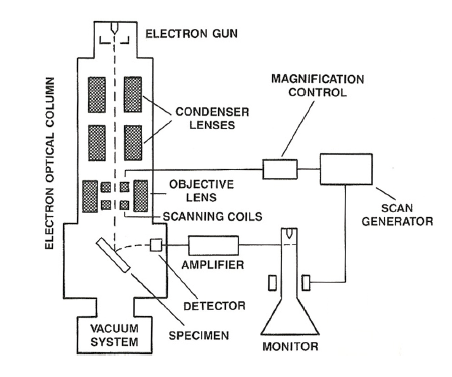
\includegraphics[width=0.6\textwidth]{Figs/Ch2/SEM.png}
	\caption {SEM design \cite{YacobiHolt1990}.}
	\label{2.4}
\end{figure}
\FloatBarrier

The electron gun generates a beam of electrons, typically of energy up to 30 keV. The condenser lenses situated below the gun serve to determine the probe size by adjusting the demagnification of the beam. The objective lens serves to further adjust this demagnification, and is situated directly above the specimen. The scanning coils serve to raster the electron probe across the sample, and the detector thus builds an image of the specimen by collecting various signals which occur due to the electron-specimen interactions.\\
As the beam of electrons interacts with the specimen, various processes occur which generate characteristic signals, as shown in Fig.\ref{2.5}. The volume within the sample which contains the energy deposited by the electron beam is known as the interaction volume, the shape and size of which is determined by both the beam energy and sample composition. Inelastic scattering of the electrons results in the production of signals such as secondary electrons \nomenclature[z-SE]{SE}{Secondary Electron} (SEs), Auger electrons and characteristic X-rays. Typically, it is the SEs which are used for imaging in SEMs. Elastic scattering can generate back scattered electrons \nomenclature[z-BSE]{BSE}{ Back Scattered Electron} (BSEs), which are collected through the surface on which the beam is incident. Due to the nature of elastic scattering, BSEs have a strong dependence on atomic, and are can thus be used to produce composition-dependent image contrast.

\begin{figure}[h]
	\centering
	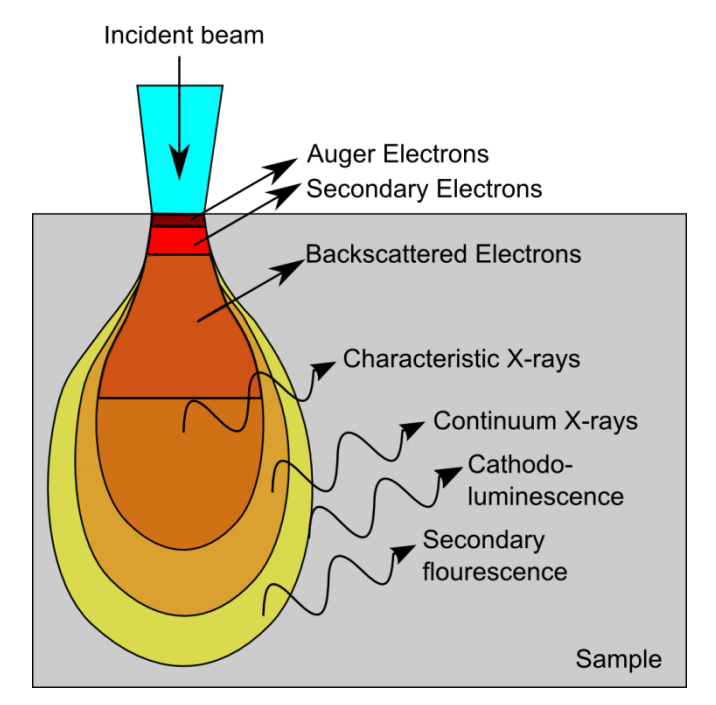
\includegraphics[width=0.6\textwidth]{Figs/Ch2/int.png}
	\caption {Interaction volumes for different interactions of an electron beam \cite{Puchtler2014}.}
	\label{2.5}
\end{figure}
\FloatBarrier



\subsubsection{Cathodoluminescence}

The absorption of primary electrons in a semiconductor can generate electronic excitations, or electron-hole pairs, with light emission occurring as a consequence of their recombination. This process is known as cathodoluminescence \nomenclature[z-CL]{CL}{Cathodoluminescence}(CL). The electronic transitions which are associated with CL emission require lower energies than those needed to excite X-rays.\\
\indent One of the principal advantages of CL in comparison with photo-excitation spectroscopy techniques used on semiconductors such as photoluminescence \nomenclature[z-PL]{PL}{Photoluminescence} (PL) is the limitation of the spatial resolution of the technique by the interaction volume of the elecctron beam in the material rather than diffraction which can be considered an intrinsic limitation of most optical far-field techniques \cite{Edwards2011}. As a result, nanometre-scale characterization of materials can be achieved.\\
\indent Due to the large number of electron-hole pairs generated within the interaction volume of the impinging electron beam on a bulk semiconductor material,all possible transitions within the material tend to be excited, resulting in the crucial limitation of being unable to selectively excite transitions below a certain energy \cite{Edwards2011}. Nonetheless, the versatility of CL as a technique has been amply demonstrated in its ability to shed light on the composition of compound materials such as InGaN/GaN structures \cite{Martin2004}, carrier diffusion length and surface recombination rates \cite{Sercel1989} and even minority carrier lifetimes \cite{YacobiHolt1990}.\\
\indent A schematic view of a set-up for CL imaging is show in Fig.\ref{2.6}:

\begin{figure}[!ht]
	\centering
	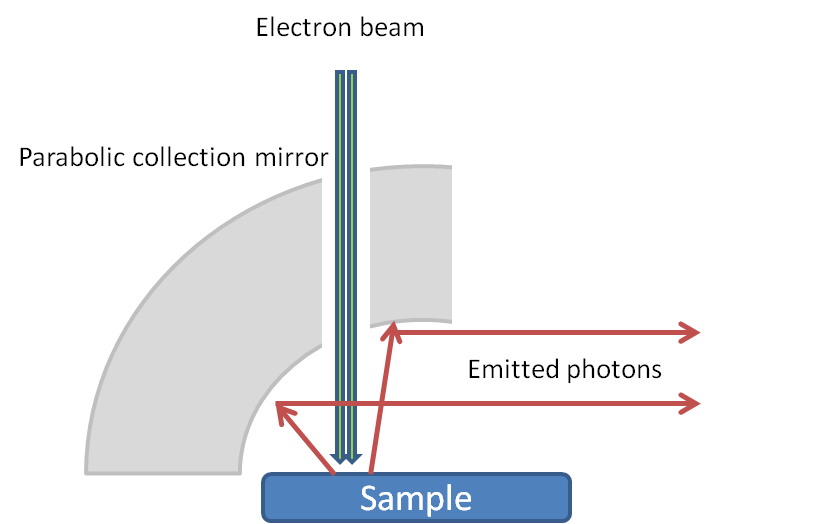
\includegraphics[width=0.5\textwidth]{Figs/Ch2/CL.png}
	\caption[h] {Schematic layout of a CL imaging system.}
	\label{2.6}
\end{figure}
\FloatBarrier

The electron beam is incident on the sample in the SEM chamber and results in the generation of photons which are collected by a parabolic mirror through a high vacuum feedthrough and coupled into a monochromator. Photomultiplier tubes (PMTs) are the most commonly used detector for this set-up. \\
The most basic form of CL imaging is known as panchromatic imaging. In this case, the collected light in its entirety is directed to a single detector and the resulting greyscale image intensity is the product of the spectral response of the system and the emission spectrum \cite{Edwards2011}. An extension of this is the monochromatic imaging mode, in which case only a single band of wavelengths is imaged using a band-pass filter or spectrometer \cite{Edwards2011}.\\
CL hyperspectral imaging, or CL wavelength imaging (CLWI) is an extension of the aforementioned technique whereby a full luminescence spectrum is recorded at each point during a beam scan, enabling the construction of a spatially and spectrally resolved data set.\\
 In the set-up shown in Fig \ref{2.6}, a semiparaboloidal mirror allows emitted photons to be collected over close to the entire hemisphere. In this case, the beam is scanned across the sample in order to achieve CL hyperspectral imaging, however a number of drawbacks are inherent to this collection geometry:\\
\\\indent - The position of the mirror requires a large working distance and can obscure the optical element thus compromising the imaging capabilities of the microscope.\\
\\\indent - The small distance between the sample and mirror imposes a restriction on the extent to which the sample can be tilted, which can be an issue in the examination of three-dimensional structures.\\
\\\indent - The {\it\'{e}tendue} of the system imposes a strict compromise between the field of view of the microscope and the collection efficiency at the spectrometer \cite{Edwards2011}.\\
\\\indent In an effort to overcome these limitations, CL hyperspectral imaging systems have been developed, whereby light collection is achieved using an objective placed perpendicular to the electron beam as shown below in Fig \ref{2.7}. By allowing the optics to be placed further away from the sample, a far shorter working distance can be used, allowing the electron spot to remain small at low accelerating voltages \cite{Edwards2011}. 

\begin{figure}[!ht]
	\centering
	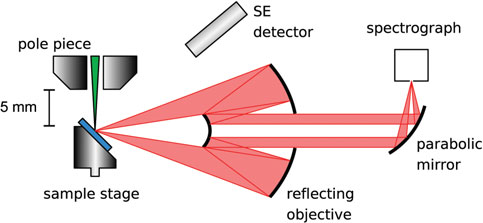
\includegraphics[width=0.5\textwidth]{Figs/Ch2/hyper.png}
	\caption[h] {Schematic layout of a CL hyperspectral imaging system \cite{Edwards2012}.}
	\label{2.7}
\end{figure}
\FloatBarrier

\subsubsection{Electron-Beam Induced Current}

Electron beam induced current \nomenclature[z-EBIC]{EBIC}{Electron-Beam Induced Current} (EBIC) imaging is a technique complementary to scanning electron microscopy. The premise of the measurement is that minority carriers which arise from the incident electron beam of an SEM on a semiconductor junction can diffuse to the junction where they are separated by the built-in field and collected as current by an external circuit (the EBIC amplifier).\\
Due to the small interaction volumes achievable, EBIC can provide detailed spatial information on minority carrier dynamics. Regions of high signal indicate high collection efficiency and low recombination, for example: the depletion region of a p-n junction appears bright in EBIC imaging. As such EBIC imaging has proven extremely useful in characterising the recombination properties of individual defects across a wide range of semiconductors \cite{Yakimov2002}.  


\section{Hyperspectral Electroluminescence Mapping}
\section{Photoluminescence}
\section{Dual Beam Scanning Electron microscopy with a Focussed Ion Beam}
\subsection{Fabrication}
\subsection{Tomography}
\section{Transmisson Electron Microscopy}
\subsection{Tomography}



%*******************************************************************************
%****************************** Third Chapter *********************************
%*******************************************************************************

\chapter{Inhomogeneous Electroluminescence in InGaN QW LEDs}

\ifpdf
    \graphicspath{{Chapter2/Figs/Raster/}{Chapter2/Figs/PDF/}{Chapter2/Figs/}}
\else
    \graphicspath{{Chapter2/Figs/Vector/}{Chapter2/Figs/}}
\fi


\section[Short title]{Background}

% Uncomment this line, when you have siunitx package loaded.
%The SI Units for dynamic viscosity is \si{\newton\second\per\metre\squared}.

$\mathrm{In_{x}Ga_{1-x}N}$/GaN QW structures are key structures in present day light emitting diodes in the visible wavelengths. Despite the growth of III-nitride LEDs into a gigantic market with a projected overall worth of 64 billion EUR by 2020, III-nitride alloys suffer from a plethora of material issues arising from heteroepitaxial growth on foreign substrates with large lattice mismatches \cite{Bennett2010b} such as the formation of defects, as mentioned in section \ref{section1.1.4}. As discussed in section \ref{section1.1.4}, whilst III-nitride optoelectronic devices appear relatively robust to dislocations relative to other III-V devices, threading dislocations can nonetheless be source of highly undesirable effects in diode structures.\\
Threading dislocations have been shown to result in inverted pyramidal defects at the surface of nitride epilayers, known as 'V defects'. The effect of these defects on LED performance is hotly debated in literature as they are expected by many to hinder LED performance, as previously discussed in section \ref{v-pit section}. However, it has been shown that narrower QWs along the sidewalls of V-defects serve to screen carriers from the non-radiative centres at TDs \cite{Hangleiter2005}.\\
In this study, a 'multi-microscopy' approach, whereby several microscopy techniques are utilised on the same features, is used to elucidate the origin of inhomogeneous EL in $\mathrm{In_{x}Ga_{1-x}N}$/GaN QW structures. The correlation of emissive and structural properties at the surface of the LED structures using several microscopy techniques has allowed for the detection of hexagonal defects at the centre of the inhomogeneities. Following this, structural and compositional information obtained using a combination of techniques is used to simulate and reproduce the inhomogeneous EL, thus elucidating the mechanism whereby hexagonal defects can cause inhomogeneous EL in LEDs.


\section{Sample Structure}
For this study, a QW InGaN LED structure with a nominal QW thicknesses of 4.5 nm was studied.The sample was grown at the Cambridge Centre for Gallium Nitride, with LED processing carried out at the University of Bath. The structure was grown on a low dislocation density \nomenclature[z-LDD]{LDD}{Low Dislocation Density} ($5 \times 10^{8}cm^{-2}$) GaN template on sapphire, and consists of a 2 $\mu m$ layer of unintentionally doped GaN followed by a 3 $\mu m$ silicon doped GaN layer. The active layer consists of a 5 period InGaN/GaN MQW region, with unintentionally doped GaN barriers (7.6 nm). An AlGaN electron blocking layer \nomenclature[z-EBL]{EBL}{Electron Blocking Layer} (20 nm) and a magnesium-doped GaN cap (117 nm) were grown following the active region. The sample code is C5608A. This is shown schematically in Fig. \ref{LEDstruct}:

\begin{figure}[!ht]
	\centering
	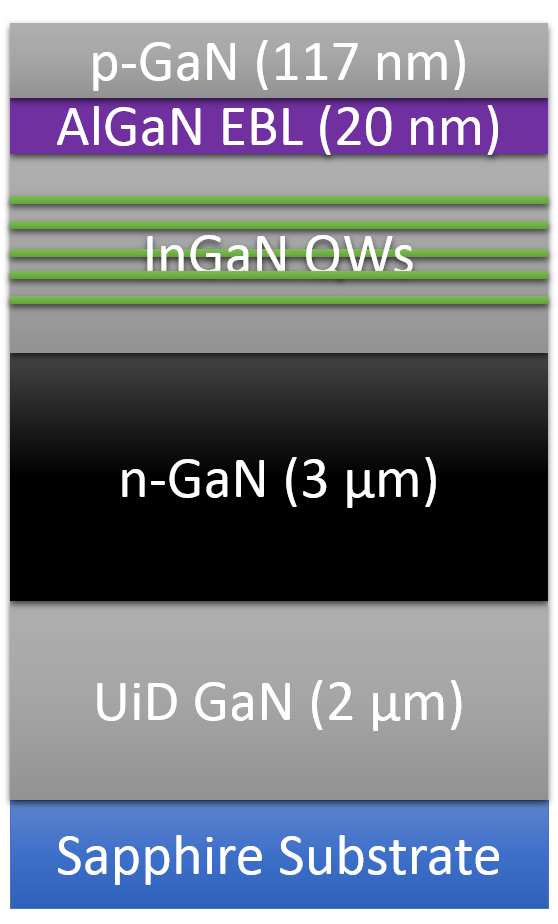
\includegraphics[width=0.4\textwidth]{Figs/Ch3/LEDstruct}
	\caption[h] {LED structure schematic.}
	\label{LEDstruct}
\end{figure}

\FloatBarrier 
The wafer was processed into $1 \times 1 mm^{2}$ side contacted LEDs with thin oxidized Ni/Au current spreading {\it p}-layer Ohmic contact. Ti/Al Ohmic contact stripes were deposited on the {\it n}-layer and the Ni/Au current spreading layer in an interdigitated geometry.\\
QW thickness for the sample was determined from X-ray diffraction \nomenclature[z-XRD]{XRD}{X-ray Diffraction} (XRD) using the method described by Vickers {\it et al.} \cite{Vickers2003}. The QWs were grown using the '2T' method, whereby the growth temperature is ramped up immediately following the InGaN growth under ammonia but without metalorganic fluxes. The barrier growth begins towards the end of the temperature ramp, this typically leads to loss of indium during the temperature ramp which can cause gross well-width fluctuations \cite{Laak2013} but a higher barrier growth temperature is preferable\cite{Oliver2013}. '2T' growth is shown schematically in Fig.\ref{2T}.

\begin{figure}[!ht]
	\centering
	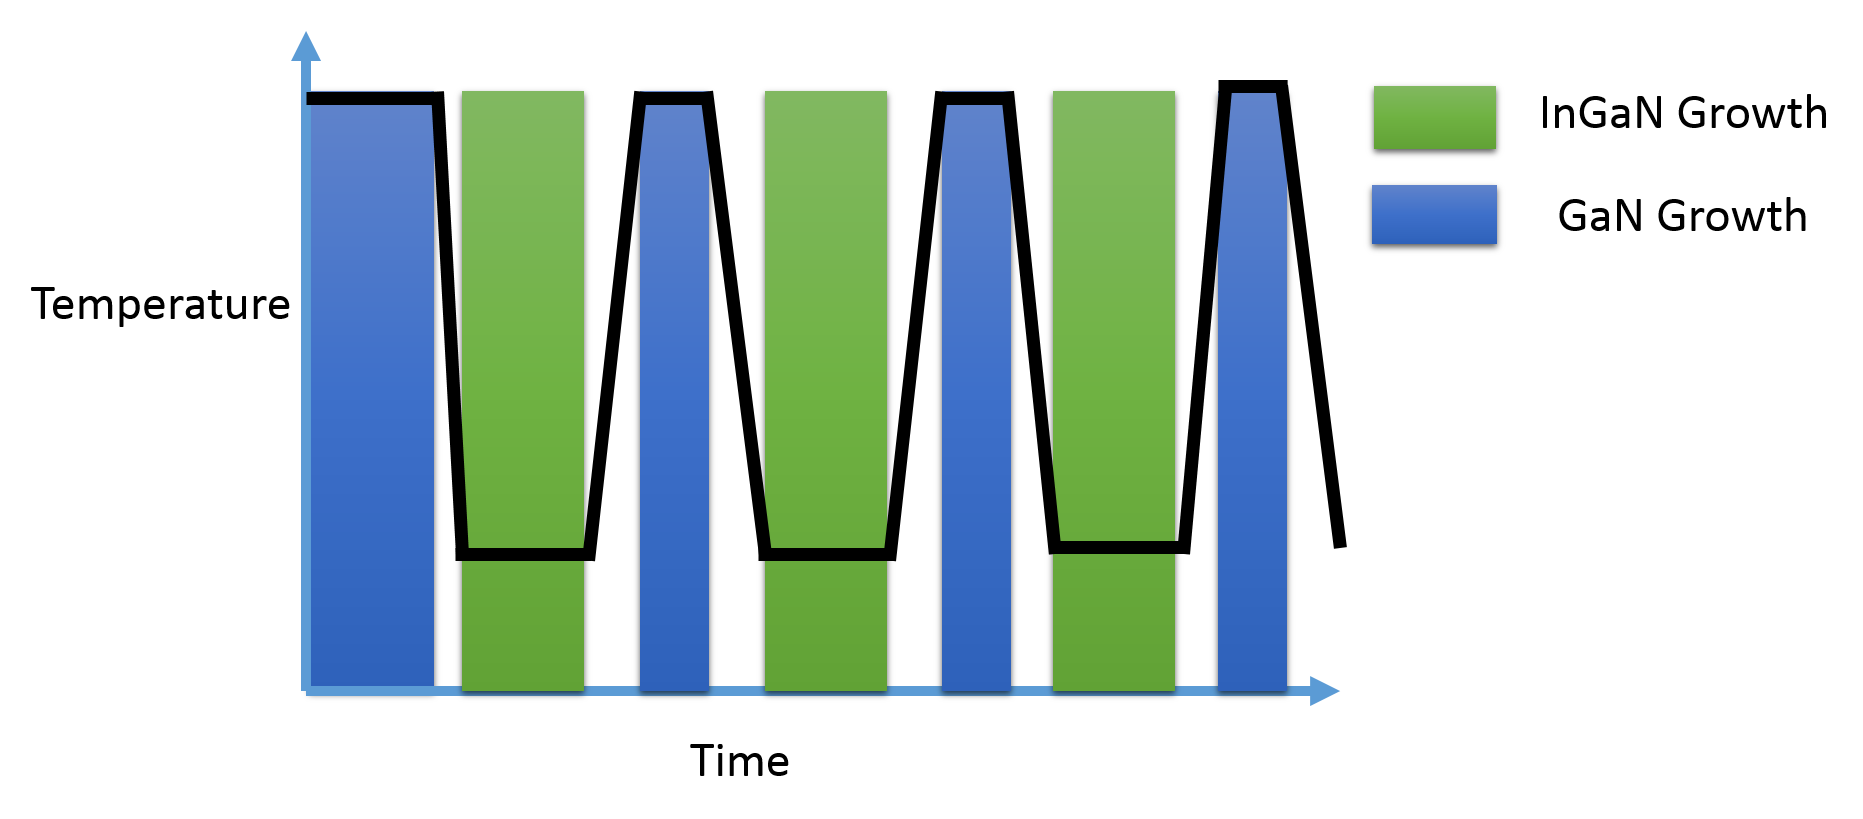
\includegraphics[width=0.9\textwidth]{Figs/Ch3/2T}
	\caption[h] {'2T' growth of InGaN/GaN QWs. GaN QB growth is halted during the temperature ramp. The black trace indicates growth temperature over time.}
	\label{2T}
\end{figure}

\FloatBarrier 

\section{Experimental}

Initial evaluation of the inhomogeneous EL was performed in a Signatone S-1160 probe station under forward bias, as shown in Fig.\ref{probe}.

\begin{figure}[h]
	\centering
	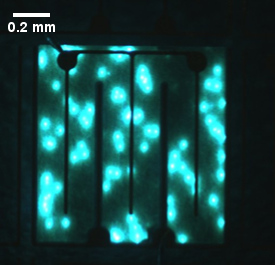
\includegraphics[width=0.4\textwidth]{Figs/Ch3/5608.png}
	\caption {LED EL under a forward bias of 3V. The bright inhomogeneities are visible in the emission of the LEDs. }
	\label{probe}
\end{figure}
\FloatBarrier


Following this, hyperspectral EL mapping with CL and EBIC were performed using a modified Cameca SX100 electron probe micro-analyser with a custom built cathodoluminescence set-up. Hyperspectral EL measurements were performed under forward bias, enabling the acquisition spatially resolved EL maps of the inhomogeneities. Following the detection of hexagonal defects at the centre of inhomogeneities using SEM-CL, the defects were analyzed using AFM and C-AFM. Finally, FIB/SEM lamella preparation techniques were used to perform HAADF-STEM and STEM-EDX on the defects, allowing for access nanoscale compositional and structural information required to reproduce the EL in simulations.


\subsection{Hyperspectral EL Imaging}
Hyperspectral EL imaging was performed at Strathclyde University with the assistance of Dr Michael Wallace. In order to study the device under forward current, the LED wafers were mounted on TO-5 headers and bonded with 5 µm Al wire. A Keithley Instrument 2401 source meter was used to apply varying forward currents to the devices and thus allow for the collection of EL. \\
Full EL spectra were collected with a spatial resolution of approximately 3 µm and analysed using custom software developed by Dr. Paul Edwards, allowing for 2-D maps of EL peak intensity, position and FWHM. At each pixel in the map, a full EL spectrum was collected by an Andor CCD spectrograph. A full set of data extracted from the hyperspectral EL mapping (taken from the background emission of the LED, and not the bright inhomogeneities) is shown in Fig.\ref{ELfull}

\begin{figure}[!ht]
	\centering
	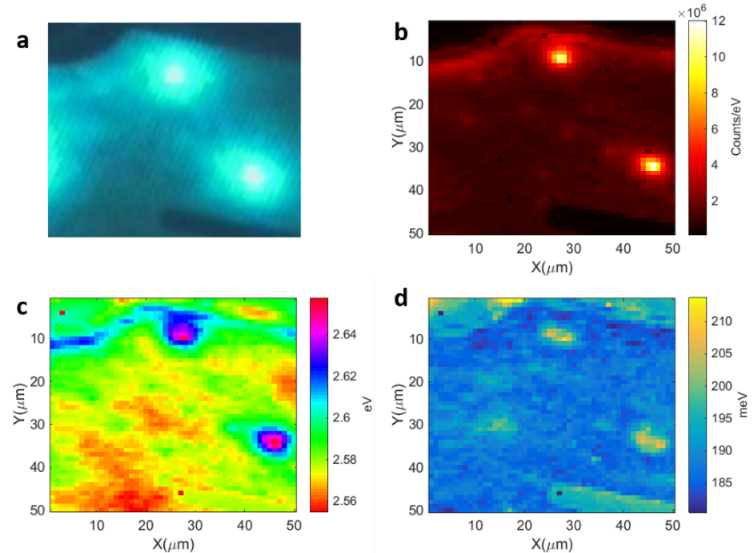
\includegraphics[width=0.8\textwidth]{Figs/Ch3/ELfull}
	\caption[h] {a) Probe station image b) EL peak intensity, c) EL peak energy and d) EL FWHM extracted by fitting the hyperspectral EL data under a forward current of 10 mA}
	\label{ELfull}
\end{figure}

\FloatBarrier 

It is interesting to note that from this representative data set, the inhomogeneities observed are brighter by a factor of $\sim 6$, blue-shifted in terms of peak energy by $\sim 0.08$ eV and have a larger FWHM. Although these values were observed to shift based on injection current, the overall trend observed in the EL data collected for this LED is represented by Fig.\ref{ELfull}.\\
All intensity measurements performed on the system at Strathclyde University (for both CL and EL) are reported with units of 'Counts/eV' due to non-uniformity between neighbouring CCD channels in the spectrograph.

\subsubsection{Current Dependent EL Measurements}

Current dependent hyperspectral EL maps of the same area were performed, in order to examine the behaviour of the inhomogeneities with increasing current relative to the 'uniform' background. The peak intensities and peak energies for injection currents for device C5608A ranging from 1-250 mA are shown in Figures \ref{peak5610} and \ref{centre5610} respectively. 

\begin{figure}
	\begin{subfigure}[b]{0.48\textwidth}
		\centering
		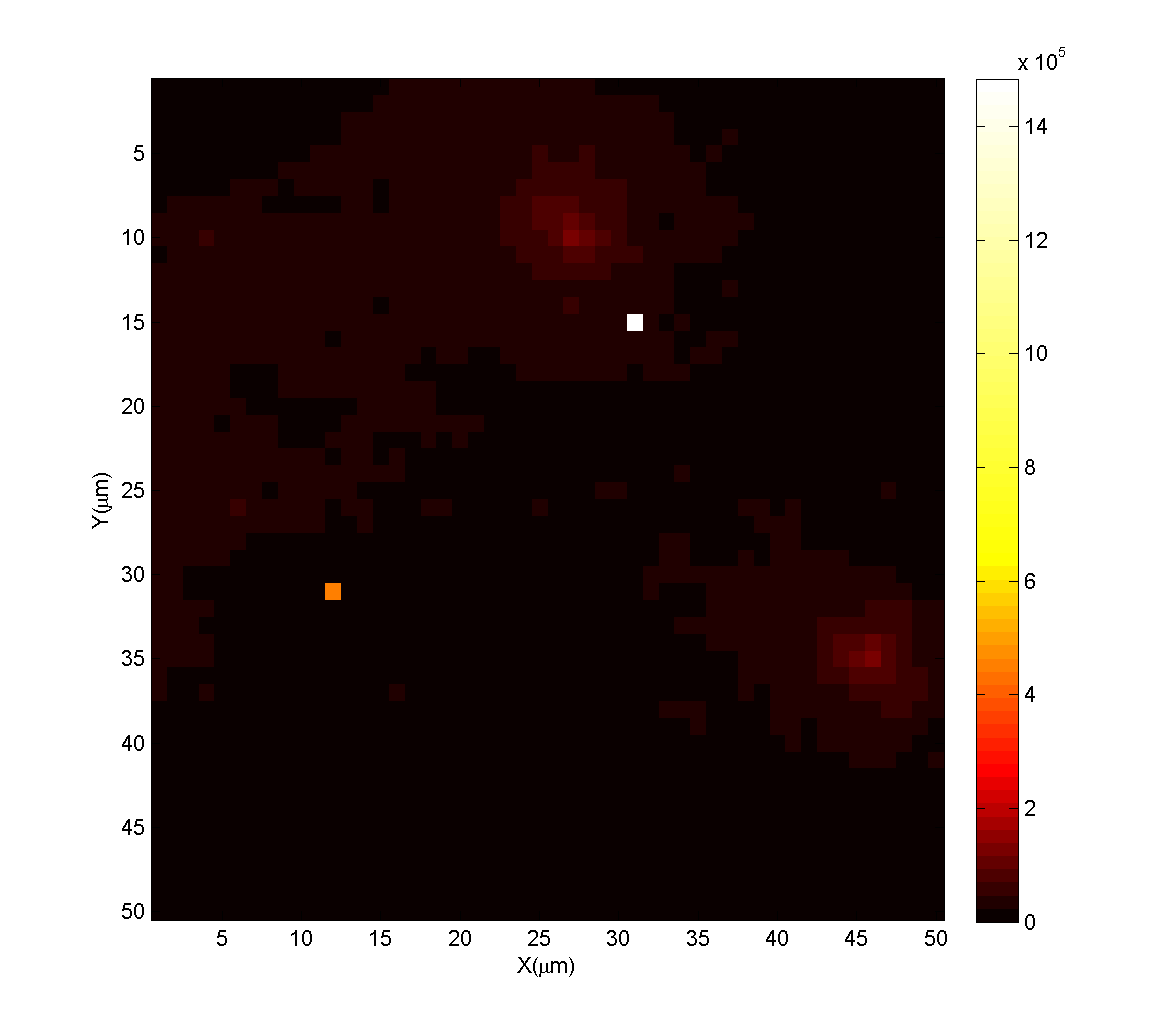
\includegraphics[width=1\linewidth]{Figs/Ch3/1c}
		\caption{1 mA}
	\end{subfigure}%
	\hspace*\fill
	\begin{subfigure}[b]{0.48\textwidth}
		\centering
		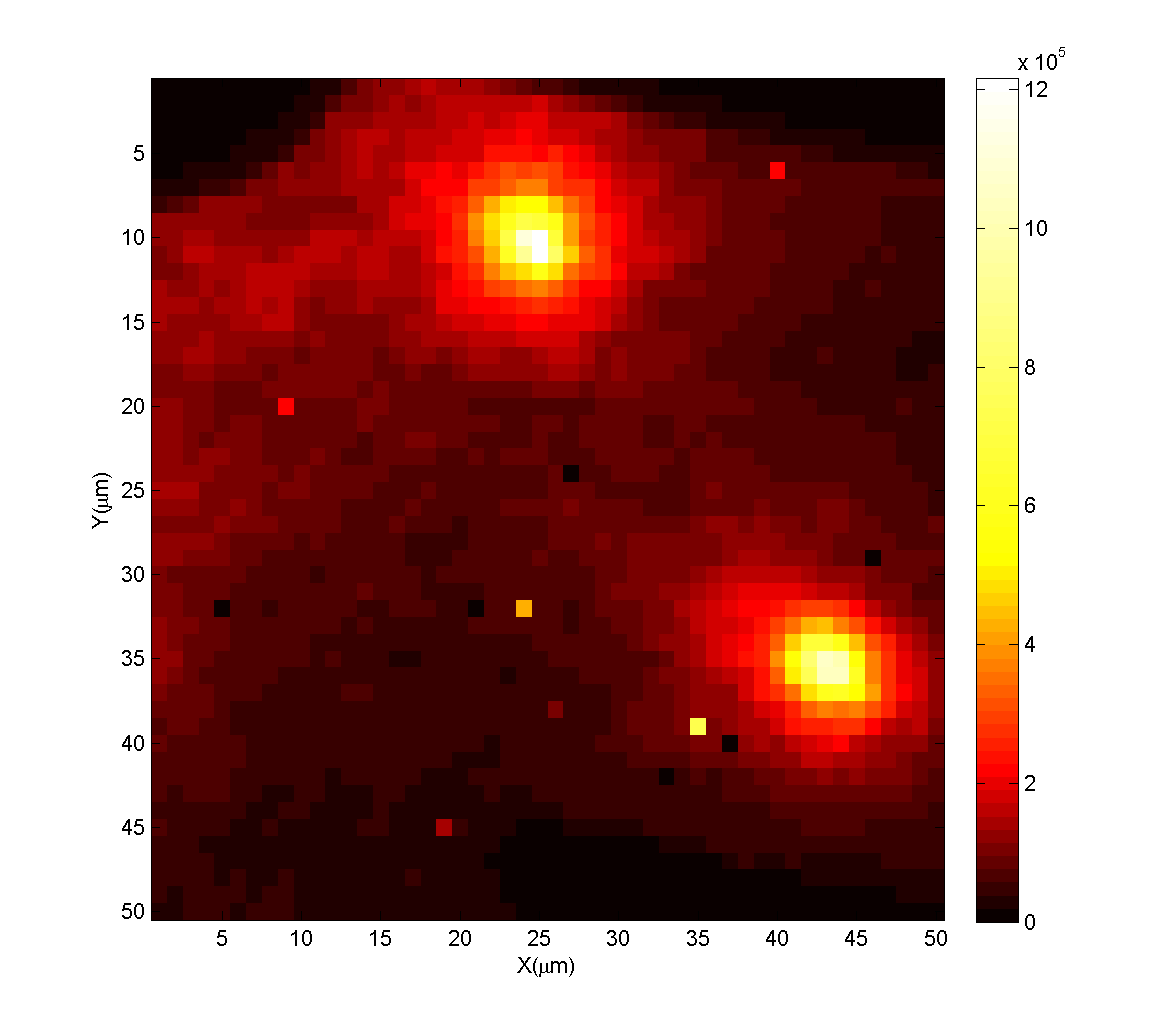
\includegraphics[width=1\linewidth]{Figs/Ch3/2dot5c}
		\caption{5 mA}		
	\end{subfigure}%
	
	\medskip
	\begin{subfigure}[b]{0.48\textwidth}
		\centering
		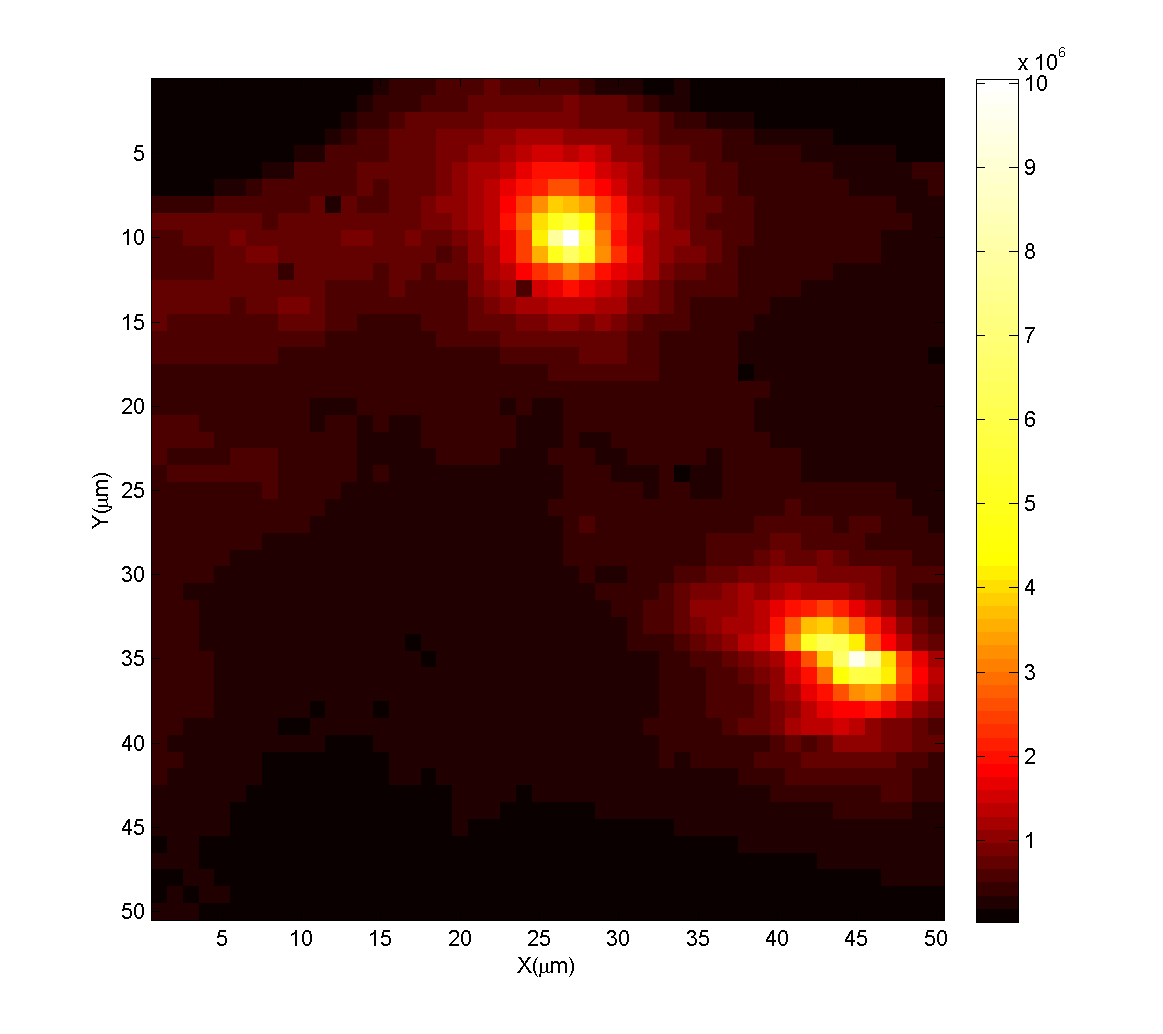
\includegraphics[width=1\linewidth]{Figs/Ch3/10c}
		\caption{10 mA}
	\end{subfigure}%
	\hspace*\fill
	\begin{subfigure}[b]{0.48\textwidth}
		\centering
		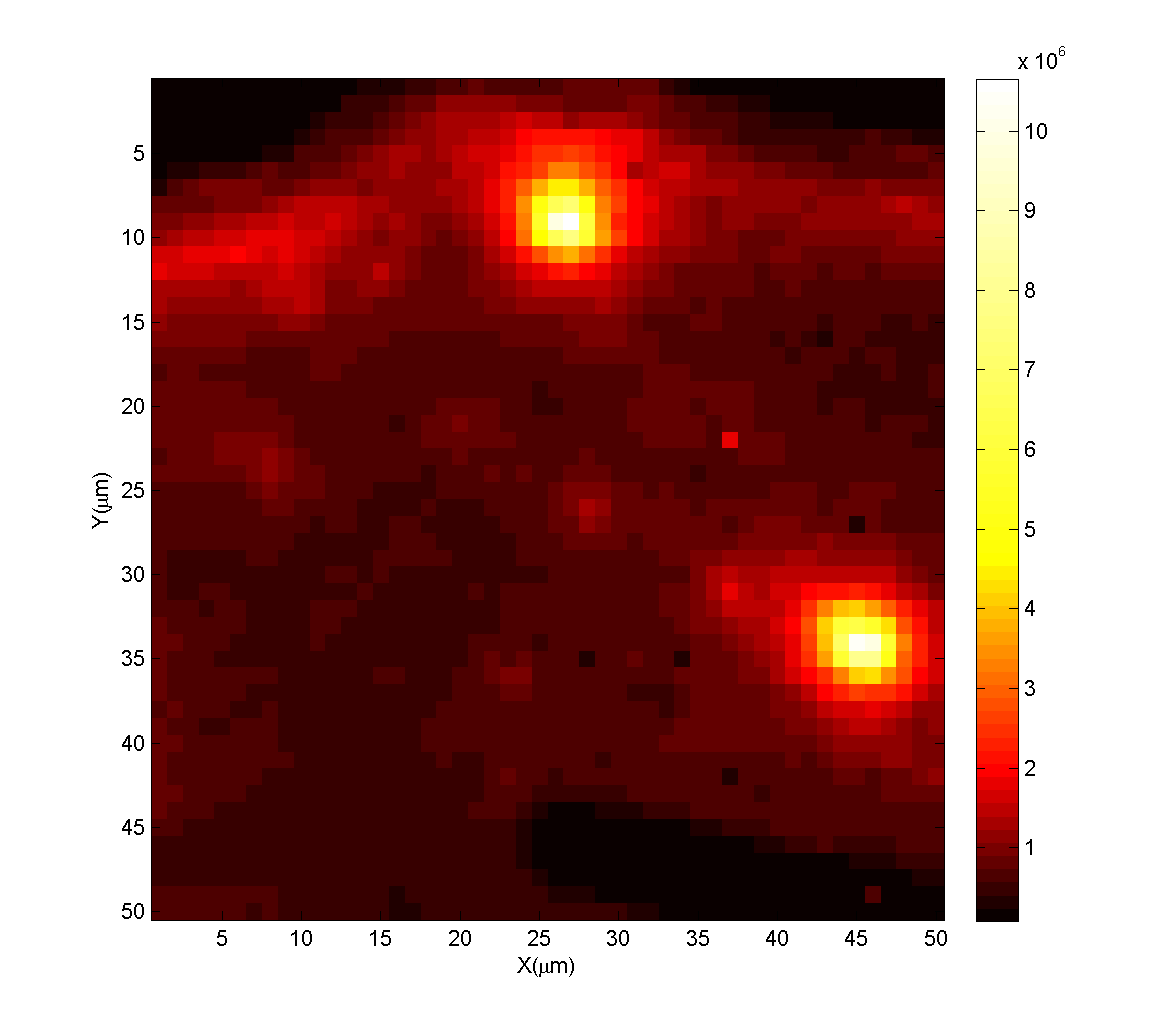
\includegraphics[width=1\linewidth]{Figs/Ch3/50c}
		\caption{50 mA}		
	\end{subfigure}%
	
	\medskip
	\begin{subfigure}[b]{0.48\textwidth}
		\centering
		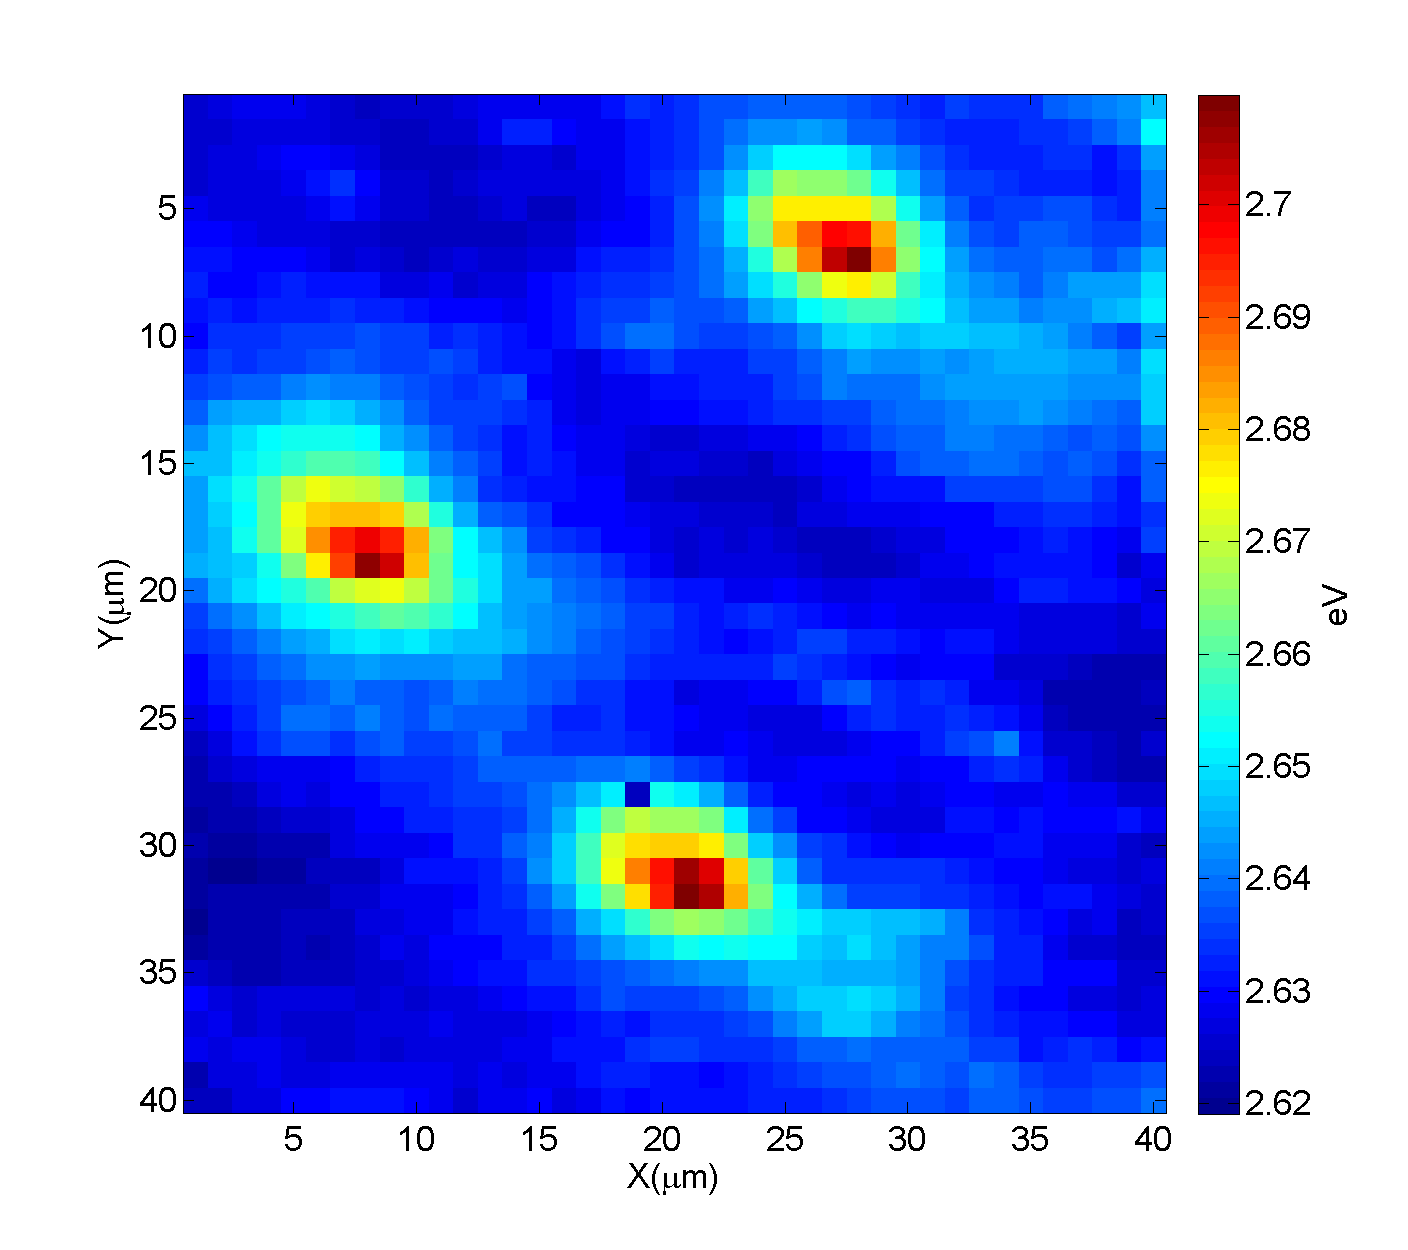
\includegraphics[width=1\linewidth]{Figs/Ch3/100c}
		\caption{100 mA}
	\end{subfigure}%
	\hspace*\fill
	\begin{subfigure}[b]{0.48\textwidth}
		\centering
		\includegraphics[width=1\linewidth]{Figs/Ch3/250c}
		\caption{250 mA}		
	\end{subfigure}%
	
	\caption{Peak intensity for varying injection current for C5608.}
	\label{peak5610}
\end{figure}

\begin{figure}
	\begin{subfigure}[b]{0.48\textwidth}
		\centering
		\includegraphics[width=1\linewidth]{Figs/Ch3/1}
		\caption{1 mA}
	\end{subfigure}%
	\hspace*\fill
	\begin{subfigure}[b]{0.48\textwidth}
		\centering
		\includegraphics[width=1\linewidth]{Figs/Ch3/5}
		\caption{5 mA}		
	\end{subfigure}%
	
	\medskip
	\begin{subfigure}[b]{0.48\textwidth}
		\centering
		\includegraphics[width=1\linewidth]{Figs/Ch3/10}
		\caption{10 mA}
	\end{subfigure}%
	\hspace*\fill
	\begin{subfigure}[b]{0.48\textwidth}
		\centering
		\includegraphics[width=1\linewidth]{Figs/Ch3/50}
		\caption{50 mA}		
	\end{subfigure}%
	
	\medskip
	\begin{subfigure}[b]{0.48\textwidth}
		\centering
		\includegraphics[width=1\linewidth]{Figs/Ch3/100}
		\caption{100 mA}
	\end{subfigure}%
	\hspace*\fill
	\begin{subfigure}[b]{0.48\textwidth}
		\centering
		\includegraphics[width=1\linewidth]{Figs/Ch3/250}
		\caption{250 mA}		
	\end{subfigure}%
	
	\caption{Peak energy for varying injection current for C5608.}
	\label{centre5610}
\end{figure}

\FloatBarrier

The spatially resolved EL data shown in Figures \ref{peak5610} and \ref{centre5610} allow for the comparison between areas containing the inhomogeneities and the 'background' EL. This is demonstrated in Fig. \ref{5610peakcomp} which shows the behaviour of both the inhomogeneities (labelled 'spots') and the averaged background peak intensity with increasing injection current.
\begin{figure}[!ht]
	\centering
	\includegraphics[width=0.8\textwidth]{Figs/Ch3/Peakcomp5608.png}
	\caption[h] {Spot and background average peak intensity against injection current}
	\label{5610peakcomp}
\end{figure}

\FloatBarrier 
It is interesting to note that Fig.\ref{5610peakcomp} shows the inhomogeneities experience a far sharper initial increase in peak intensity relative to the background based on the hyperspectral EL data fitting in the current range 0-50 mA, perhaps indicating enhanced current injection in the areas exhibiting the inhomogeneities.\\
Fig. \ref{5610centrecomp} shows the same current dependent comparison for background and inhomogeneity peak energy. Here we see the same trend, in that the inhomogeneity exhibits a larger current-induced blueshift in the 0-50 mA range relative to the background. The origin of the current-dependent blueshift in InGaN QW structures is attributed to the screening of the QCSE by the additional carriers injected into the wells \cite{Ryou2009}, and as such indicates the inhomogeneities are regions experiencing higher current injection relative to the background.

\begin{figure}[!ht]
	\centering
	\includegraphics[width=0.8\textwidth]{Figs/Ch3/centrePeakcomp5608.png}
	\caption[h] {Spot and background average peak energy against injection current}
	\label{5610centrecomp}
\end{figure}

\FloatBarrier 


\subsection{Cathodoluminescence and Electron Beam Induced Current}
Having noted the behaviour of the inhomogeneities inferred from the hyperspectral EL data, CL and EBIC data were taken over areas containing the inhomogeneities in order to examine their properties in more detail as electron-beam based techniques allow for a far higher resolution than EL mapping.\\
In order to achieve simultaneous CL and EBIC measurements, a Keithley Instrument 2401 source/measure unit was utilised in order to main the LED devices at a fixed bias of 0V thus allowing for the measurement of the short circuit current. During the CL image scanning, the Andor CCD camera was set-up to trigger the unit to record the current at each point in the CL spectral acquisition. The CL acquisition was performed with an electron beam at 10 kV and 1 nA. Unfortunately the secondary electron detector was inoperable during the acquisition of this data, as such there is no accompanying SEM micrograph for the CL and EBIC data. The CL and EBIC data for C5608A are shown in Fig.\ref{5608CLEBIC}.

\begin{figure}[h]
	\hspace*{0.5cm}
	\begin{subfigure}[b]{0.48\textwidth}
		\centering
		\includegraphics[width=1\linewidth]{Figs/Ch3/5608AsmallCL}
		\caption{}
		
	\end{subfigure}%
	\hspace*{0.5cm}
	\begin{subfigure}[b]{0.48\textwidth}
		\centering
		\includegraphics[width=0.98\linewidth]{Figs/Ch3/5608smallEBIC}
		\caption{}
	\end{subfigure}%
	
	\caption{a) CL and b) EBIC maps acquired simultaneously of the area shown in Fig.\ref{5610loc}b.}
	\label{5608CLEBIC}
\end{figure}
\FloatBarrier

Fig. \ref{5608CLEBIC}a. shows the inhomogeneities exhibit a lower CL intensity relative to the background, in contrast to the EL. Interestingly, the EBIC signal, shown in Fig.\ref{5608CLEBIC} for both inhomogeneities examined seem rather different. The feature closest to the contact region can be seen as a region of high EBIC surrounding a region of lower extracted current. \\
The low CL intensity detected can be interpreted in several manners: a high density of TDs or point defects could result in non-radiative recombination in these areas \cite{Polyakov1998,Bennett2010b} or enhanced stress in these regions could result in an enhancement of the QCSE which in turn would redshift and reduce the intensity of the CL emission \cite{Ren2015,Ryou2009}. The enhanced EBIC in these regions tends to suggest the latter is more likely: the strain enhanced piezoelectric field across the QW stack would likely separate generated carrier-pairs \cite{Chichibu1999} and result in a higher EBIC relative to the less-strained background. 

\subsubsection{Scanning Electron Microscopy with Cathodoluminescence}

Following the CL and EBIC scans shown in Fig.\ref{5608CLEBIC} performed at Strathclyde University, more detailed SEM-CL experiments were performed at the University of Cambridge using a Phillips XL30s field emission SEM at 5 kV equipped with a Gatan MonoCL4 system to record the CL signal. This set-up provides the additional benefit of panchromatic CL imaging, which allows for the detection of the features without the need for detailed EL correlation.\\
Fig. \ref{5608-SEM-CL} shows the morphology of the features in the panchromatic CL and the associated SEM micrograph. The inhomogeneity appears as a region of lower CL intensity, though it is important to note the signal in panchromatic CL mode is the sum of the complete spectrum of photons collected. Nonetheless, this can be considered in relatively good agreement with the CL intensity recorded in Fig.\ref{5608CLEBIC}.a. Fig.\ref{5608-SEM-CL} reveals the presence of a hexagonal defect (outlined in red) which can be spatially correlated with the centre of the feature in the panchromatic CL image in Fig.\ref{5608CLEBIC}.b.

\begin{figure}[h]
	
	\begin{subfigure}[b]{0.48\textwidth}
		\centering
		\includegraphics[width=0.7\linewidth]{Figs/Ch3/5608sem}
		\caption{}
		
	\end{subfigure}%
	\hspace*{0.5cm}
	\begin{subfigure}[b]{0.48\textwidth}
		\centering
		\includegraphics[width=0.7\linewidth]{Figs/Ch3/5608panCL}
		\caption{}
	\end{subfigure}%
	
	\caption{a) SEM micrograph and b) pan-CL image of an inhomogeneity in C5608A. The pan-CL image utilises a temperature scale (blue = low, red = high).}
	\label{5608-SEM-CL}
\end{figure}
\FloatBarrier

A hyperspectral CL map of 2 $\times$ 2 $\mu m^{2}$ was taken to examine the emissive properties of the defect in more detail. Fig.\ref{11-CL}.a. shows that as expected, the region close to the hexagonal defect exhibits low CL intensity. Interestingly, the defect also shows extremely low-energy emission relative to the background, most likely due to defect-related yellow band emission \cite{Lyons2010}.

\begin{figure}[h]
	
	\begin{subfigure}[b]{0.48\textwidth}
		\centering
		\includegraphics[width=1\linewidth]{Figs/Ch3/11-peak}
		\caption{}
		
	\end{subfigure}%
	\hspace*{0.5cm}
	\begin{subfigure}[b]{0.48\textwidth}
		\centering
		\includegraphics[width=1\linewidth]{Figs/Ch3/11-centre}
		\caption{}
	\end{subfigure}%
	
	\caption{a) CL peak intensity and b) CL peak energy for the feature shown in Fig.\ref{5608-SEM-CL}}
	\label{11-CL}
\end{figure}
\FloatBarrier

\subsection{Hexagonal Defect Structure}

The structure of the hexagonal defects found at the centre of the inhomogeneities was examined following their detection using SEM-CL. 

\subsubsection{Scanning Electron Microscopy}
In order to achieve a higher resolution in examining the defects via SEM, an FEI Helios Nanolab 650 SEM/FIB with a schottky FEG at 5 kV and through lens detector (TLD) was used to perform high resolution SEM imaging. This is shown in Fig. \ref{sem-pit}.

\begin{figure}[!ht]
	\centering
	\includegraphics[width=0.8\textwidth]{Figs/Ch3/sem-pit.png}
	\caption[h] {High-resolution SEM image of a hexagonal defect located at the centre of an inhomogeneity in the EL. The vertices of the facets are delineated by dashed lines.}
	\label{sem-pit}
\end{figure}
\FloatBarrier 

Most hexagonal defects located at the centre of the inhomogeneities fell within the 200-600 nm range, with some exceedingly large defects reaching up to 1 $\mu$m in size. This is rather uncommon for hexagonal defects in III-nitrides, as the lateral size of hexagonal defects is typically sub-100 nm \cite{Oliver2006a,Tsai2007}.

\subsubsection{Atomic Force Microscopy}
The topography of the hexagonal defect was studied by AFM performed on a Veeco Dimension 3100 with RTESP tips with a nominal radius of 8 nm in intermittent contact mode. The defect shown in the SEM micrograph in Fig.\ref{sem-pit} is shown below in the AFM image.

\begin{figure}[!ht]
	\centering
	\includegraphics[width=0.7\textwidth]{Figs/Ch3/AFM.png}
	\caption[h] {AFM image of the hexagonal defect.}
	\label{afm-pit}
\end{figure}
\FloatBarrier 

By taking a topography profile across the hexagonal defect, we can resolve the depth of the defect as well as the slope of the facets.

\begin{figure}[!ht]
	\centering
	\includegraphics[width=0.5\textwidth]{Figs/Ch3/profile}
	\caption[h] {Profile taken across the defect shown in Fig.\ref{afm-pit}}
	\label{profile}
\end{figure}
\FloatBarrier 

\subsubsection{TEM Lamella preparation}
\label{FIB marker section}

Preparation of TEM lamellae for the analysis of the defects requires some additional steps due to site-specific nature of the experiment. Standard FIB/SEM sample preparation methods simply require a 2 $\mu$m thick wedge of the sample to be extracted and thinned down to a thickness of 100-200 nm for TEM experiments. However, analysis of the defect and any associated dislocations which may be present at the apex of the inverted pyramidal shape \cite{Watanabe2003,Shiojiri2006} requires thinning to be performed in an extremely controlled manner. A method devised by Thomas O'Hanlon at the Cambridge Centre for Gallium Nitride was utilised to perform high-precision site specific TEM sample preparation shown in Fig.\ref{FIBprep}. A 'marker layer' consisting of a cross intersecting the apex of the defect is deposited using the electron beam, thus allowing for little damage to the unprotected sample and a higher deposition resolution than the ion beam. Following this a protective layer is then deposited using the ion beam, and a standard dual-beam lift-out method is used to extract the wedge of sample containing the defect. 

\begin{figure}[!ht]
	\centering
	\includegraphics[width=1\textwidth]{Figs/Ch3/FIB-spot}
	\caption[h] {Marker layer deposition for high precision TEM sample preparation.}
	\label{FIBprep}
\end{figure}
\FloatBarrier 

The purpose of the marker layer is guide the sample thinning process. The electron beam deposited platinum provides contrast against both the sample and the ion-beam platinum in the SEM image. As the sample is imaged in cross-section during the thinning process, the distance between the marker layer 'ends' is an indicator of the proximity to the defect apex. As the defect apex is reached during the thinning process, the two marker stripes should merge into one at the intersection of the cross, as shown in Fig.\ref{FIBloc}.

\begin{figure}[!ht]
	\centering
	\includegraphics[width=1\textwidth]{Figs/Ch3/FIB-loc-diagram}
	\caption[h] {Marker layer deposition for high precision TEM sample preparation.}
	\label{FIBloc}
\end{figure}
\FloatBarrier 

A successfully thinned sample is shown in Fig.\ref{thinned}.

\begin{figure}[h]
	\centering
	\includegraphics[width=0.6\textwidth]{Figs/Ch3/thinned}
	\caption[h] {SEM image of a prepared TEM lamella showing the marker position and defect apex.}
	\label{thinned}
\end{figure}
\FloatBarrier 


\subsubsection{Transmission Electron Microscopy}

The site-specific TEM lamella prepared using the dual-beam methods, shown in Fig.\ref{thinned}, was studied by HAADF-STEM performed on an FEI Osiris microscope with an extreme-FEG (X-FEG) \nomenclature[z-X-FEG]{X-FEG}{Extreme Field-Emission Gun} at 200 kV. HAADF-STEM imaging of the defect reveals it originates below the MQW stack, a possible explanation for the large size of the hexagonal defects relative to those reported in literature \cite{Hangleiter2005,Tsai2007,Oliver2006a}. 

\begin{figure}[h]
	\centering
	\includegraphics[width=0.6\textwidth]{Figs/Ch3/STEM-spot}
	\caption[h] {HAADF-STEM image of a prepared TEM lamella showing defect interrupting the QW stack.}
	\label{STEM-spot}
\end{figure}
\FloatBarrier 

The composition of the MQW stack adjacent to the region occupied by the defect was studied using EDX-STEM, where the characteristic X-rays emitted by the sample were recorded by four silicon drift detectors which form a solid angle greater than 0.9 sr. Cliff-Lorimer analysis of the aluminium, gallium and indium was performed using HyperSpy in order to quantify the ternary alloy compositions as shown in Fig.\ref{EDXspot}

\begin{figure}[h]
	\begin{subfigure}[b]{0.48\textwidth}
	\centering
		\includegraphics[width=1\linewidth]{Figs/Ch3/EDStarget}
		\caption{}
	\end{subfigure}%
	\hspace*\fill
	\begin{subfigure}[b]{0.48\textwidth}
		\centering
		\includegraphics[width=1\linewidth]{Figs/Ch3/AtomicAl}
		\caption{}		
	\end{subfigure}%
	
	\medskip
	\begin{subfigure}[b]{0.48\textwidth}
		\centering
		\includegraphics[width=1\linewidth]{Figs/Ch3/AtomicGa}
		\caption{}
	\end{subfigure}%
	\hspace*\fill
	\begin{subfigure}[b]{0.48\textwidth}
		\centering
		\includegraphics[width=1\linewidth]{Figs/Ch3/AtomicIn}
		\caption{}		
	\end{subfigure}%
	

	\caption{Quantification of the ternary alloy compositions: a) HAADF-STEM image showing the region examined by EDX (blue box) b) aluminium atomic percentage, c) gallium atomic percentage and d) indium atomic percentage.}
	\label{EDXspot}
\end{figure}
\FloatBarrier 
The EDS analysis shows the disruption of the QW stack by the defect, as evidenced by the apparent termination of the QW In signal in Fig.\ref{EDXspot}.d. Additionally, the Al signal can be seen to overlap with the QW In signal, suggesting the presence of aluminium in the region disrupted by the defect. Furthermore, there is an observable indium signal originating from below the QWs. Although both the aluminium and indium atomic percentages observed in the region disrupted by the defect appear lower than expected (approximately 6-7 $\%$ and 4 $\%$ respectively) it is also important to consider the effect of the sample geometry in the collection of the EDX signal: due to the inverted pyramidal morphology of the defect the collected signal is expected to be reduced, and thus the atomic percentages obtained via quantification are expected to be under-estimates.

\subsection{LED Simulations}

In order to investigate the manner in which changes induced by the defect could affect the EL of the LED simulations were performed by Bertand Rouet-Leduc using the APSYS simulation package, with parameters taken from J.Piprek \cite{Piprek2007}. The carrier transport equations are self-consistently solved and coupled with the Schrodinger equation to compute the confined states in the QWs.\\

\subsubsection{Deep Inclusion}
Fig.\ref{simsetup} shows the simulated LED structure with a hexagonal defect incorporated. In this case we assume the QW stack simply continues along the edge of the hexagonal defect as described in \cite{Hangleiter2005}, as the EDX quantification reveals a detected atomic percentage of indium of approximately 4 $\%$ below the QW stack. We assume a similar geometry for the AlGaN EBL, which is expected to follow the angled facet of the defect. Thus, this set of simulations deals with what we term a 'deep' AlGaN inclusion, which is expected to penetrate below the QW stack. Although the atomic Al percentage shown in Fig.\ref{EDXspot}.b. below the QW stack is reduced relative to the Al percentage in the EBL, this may be due to projection artifacts related to the geometry of the hexagonal defect and the thickness of the TEM lamella.\\
In this set of simulations, we have set the {\it p}-GaN doping concentration to 3 $\times 10^{19} cm^{-3}$, the {\it p}-AlGaN EBL doping to 4 $\times 10^{19} cm^{-3}$ except on the semi-polar facets of the defect where it is set to 1$\times 10^{19} cm^{-3}$.


\begin{figure}[h]
	\centering
	\includegraphics[width=0.6\textwidth]{Figs/Ch3/Sim}
	\caption[h] {Simulated LED structure.}
	\label{simsetup}
\end{figure}
\FloatBarrier 

The simulation results are shown in Fig.\ref{simresults}.. Fig.\ref{simresults}.a. shows overall radiative recombination events in units of $10^{28} cm^{-3}s^{-1}$. The region closest to the defect at the lowest QW shows an increased radiative recombination rate, indicating the presence of the defect can indeed cause enhanced radiative recombination under electrical injection in regions surrounding the defect, in agreement with the experimental observation of inhomogeneous EL. Fig.\ref{simresults}.b. shows two profiles taken from Fig.\ref{simresults}.a. intersecting the five QWs and indicates that the rate of radiative recombination is almost doubled in the lowest QW close to the defect when compared with a profile taken further away.\\
Under closer examination, Fig.\ref{simresults}.b. demonstrates that the 'bottom' QW dominates the overall emission, particularly close too the AlGaN inclusion. The carrier concentrations shown in Figures.\ref{simresults}a. and b show that this is primarily due to the enhanced hole concentration in the region adjacent to the AlGaN, as the electron concentration is relatively unchanged. Thus we can ascribe the enhanced local carrier concentration to the presence of the \textit{p}-AlGaN, which injects holes directly into the active region. The effects of hexagonal defect-assisted carrier injection into MQW stacks have been reported by Li \textit{et al.}, who reported that the disruption of the MQW stack by the hexagonal defect combined with thinner QBs allowed for the injection of holes up to 8 pairs of QWs away from the \textit{p}-GaN \cite{Li2014}. Quan \textit{et al.} have also suggested that hole injection via the semi-polar facets of the hexagonal defect occurs at a higher rate resulting in high radiative recombination near the defect, but larger defects may result in localised emission \cite{Quan2014}.

\begin{figure}[h]
	\begin{subfigure}[b]{0.45\textwidth}
		\centering
		\includegraphics[width=1\linewidth]{Figs/Ch3/deep}
		\caption{}
	\end{subfigure}%
	\hspace*\fill
	\begin{subfigure}[b]{0.49\textwidth}
		\centering
		\includegraphics[width=1\linewidth]{Figs/Ch3/150rad}
		\caption{}		
	\end{subfigure}%
	
	\medskip
	\begin{subfigure}[b]{0.49\textwidth}
		\centering
		\includegraphics[width=1\linewidth]{Figs/Ch3/150elec}
		\caption{}
	\end{subfigure}%
	\hspace*\fill
	\begin{subfigure}[b]{0.49\textwidth}
		\centering
		\includegraphics[width=1\linewidth]{Figs/Ch3/150hole}
		\caption{}		
	\end{subfigure}%
	
	
	\caption{APSYS simulation results: a) Radiative recombination events b) radiative recombination profiles, c) electron concentration profiles and d) hole concentration profiles. Red and black traces in b), c) and d) correspond to the red and black profiles in a).}
	\label{simresults}
\end{figure}
\FloatBarrier 

\subsubsection{Shallow Inclusion}

In this simulation we have simulated a structure similar to the composition maps shown in Fig.\ref{EDXspot}. We have assumed that the AlGaN EBL may penetrate only slightly in into the QW stack due to the defect, but otherwise the rest of the disrupted region is filled with undoped GaN. The AlGaN EBL doping is set to 5$\times 10^{18} cm^{-3}$ with an Al content of 10$\%$. Thus, in this case we assume no projection artifacts, as opposed to the deep Al inclusion simulated previously. The geometry used for this simulation is shown in Fig.\ref{shallowgeom}.

\begin{figure}[h]
	\centering
	\includegraphics[width=0.6\textwidth]{Figs/Ch3/shallow}
	\caption[h] {Simulated LED structure for the shallow inclusion.}
	\label{shallowgeom}
\end{figure}
\FloatBarrier 

Fig.\ref{shallowres} shows the simulation results. Fig.\ref{shallowres}.a. shows that radiative recombination is enhanced in the vicinity of the shallow inclusion, particularly in the second QW (QW2) from the EBL due to carrier injection from the semi-polar facets of the defect. Fig.\ref{shallowres}.c. and Fig.\ref{shallowres}.d. show that the hole concentration is responsible for the local enhancement in radiative recombination near the shallow inclusion as the electron concentration is mostly unchanged. Fig.\ref{shallowres} show that the enhanced injection of holes results in an order of magnitude increase in radiative recombination in QW2. As such, even in the case of a 'shallow' \textit{p}-AlGaN inclusion induced by a hexagonal defect, the injection of holes into the active region still results in enhanced emission adjacent to the defect.

\begin{figure}[h]
	\begin{subfigure}[b]{0.45\textwidth}
		\centering
		\includegraphics[width=1\linewidth]{Figs/Ch3/shallowrad1}
		\caption{}
	\end{subfigure}%
	\hspace*\fill
	\begin{subfigure}[b]{0.49\textwidth}
		\centering
		\includegraphics[width=1\linewidth]{Figs/Ch3/shallowrad}
		\caption{}		
	\end{subfigure}%
	
	\medskip
	\begin{subfigure}[b]{0.49\textwidth}
		\centering
		\includegraphics[width=1\linewidth]{Figs/Ch3/shallowelec}
		\caption{}
	\end{subfigure}%
	\hspace*\fill
	\begin{subfigure}[b]{0.49\textwidth}
		\centering
		\includegraphics[width=1\linewidth]{Figs/Ch3/shallowhole}
		\caption{}		
	\end{subfigure}%
	
	
	\caption{APSYS simulation results: a) Radiative recombination events b) radiative recombination profiles, c) electron concentration profiles and d) hole concentration profiles. Red and black traces in b), c) and d) correspond to the red and black profiles in a).}
	\label{shallowres}
\end{figure}
\FloatBarrier 

\subsection{Origin of the Defect}
In the previous sections we have established the cause of the inhomogeneous EL to be the presence of large hexagonal defects. However, it is also important to establish the origin of these hexagonal defects, as their elimination is the key to the production of LEDs with uniform emission, unlike those studied here.

\subsubsection{Threading Dislocation Analysis}

Hexagonal defects are typically associated with threading dislocations \cite{Florescu2003}, as such we performed TEM on the FIB prepared lamella in order to observe threading dislocation associated with the hexagonal defects observed at the centre of inhomogeneities in the EL. The TEM image is shown in Fig. \ref{TEM-spot}. Interestingly, rather than a single TD, we can observe a 'bundle' of dislocations associated with the defect with several 'loops' also apparent.

\begin{figure}[h]
	\centering
	\includegraphics[width=0.4\textwidth]{Figs/Ch3/TEMspot}
	\caption[h] {TEM image viewed along the $(10\bar{1}0)$ direction of the dislocations associated with the hexagonal defect shown in Fig.\ref{STEM-spot}. The scale bar corresponds to a  length of 200 nm.}
	\label{TEM-spot}
\end{figure}
\FloatBarrier 

In order to characterise the dislocations shown in Fig.\ref{TEM-spot}, WBDF-TEM was performed. The results are shown in Fig.\ref{WBDF-spot}.
\begin{figure}[h]
	\centering
	\includegraphics[width=1\textwidth]{Figs/Ch3/WBDF-yall}
	\caption[h] {WBDF-TEM of TDs associated with the hexagonal defect under a) \textbf{g}=$<11\bar{2}0>$ and b) \textbf{g}=$<0001>$. The scale bar corresponds to a length of 150 nm.}
	\label{WBDF-spot}
\end{figure}
\FloatBarrier 

Fig.\ref{WBDF-spot} shows that the majority of TDs associated with the pit are mixed in nature, with some exceptions such as the 'dislocation loop' which shows no contrast under when viewed under the condition \textbf{g}=$<0001>$. Nonetheless, the number of TDs associated with a single defect here is astonishing.\\
The bundle of TDs observed here could potentially be attributed to the vertical side facets in GaN islands during the inital growth of the GaN template on sapphire. Datta \textit{et al.} showed that threading dislocations associated with basal plane stacking faults are located at coalescence boundaries between two GaN grains, and can open up into hexagonal defects at the surface, as shown in Fig.\ref{Datta} \cite{Datta2004}. In order to avoid GaN grains with vertical side facets, Datta \textit{et al.} suggest initialising epilayer growth at a low V/III ratio or increased pressure as these conditions favour the formation of GaN islands with inclined side facets\cite{Hiramatsu2001,Beaumont1999}, thus allowing TDs to bend laterally during film coalescence rather than propagate upwards towards the epilayer surface and form hexagonal defects.

\begin{figure}[h]
	\centering
	\includegraphics[width=1\textwidth]{Figs/Ch3/Datta}
	\caption[h] {BF-TEMimage of a coalescence boundary between two GaN grains and associated threading dislocations opening up into a hexagonal defect \cite{Datta2004}. }
	\label{Datta}
\end{figure}
\FloatBarrier 


\section{Conclusion}

First and foremost we have utilised a host of microscopy techniques to identify the cause of inhomogeneous EL in III-nitride LEDs. Hyperspectral EL mapping was performed over a set of inhomogeneities in order to determine their spectral properties. Using this data, the inhomogeneities were established to be blueshifted and have a larger emission FWHM. Further current dependent EL-measurements revealed that the inhomogeneities exhibited emissive properties consistent with higher local carrier concentration.\\
SEM-based techniques were used to further elucidate the properties of the inhomogeneities. Panchromatic CL was used to reveal dark regions surrounding the inhomogeneities, as well as hexagonal defects at the centre of the inhomogeneities.\\
A FIB-based technique to deposit marker layers was used in order to produce a TEM lamella through the apex of a hexagonal defect at the centre of an inhomogeneity. This allowed for STEM-EDX mapping of the region surrounding the defect apex, revealing the presence of Al from the AlGaN EBL in the active region.\\
APSYS simulations were performed in order to examine the effect of AlGaN penetrating within the active layer for both a 'deep' (penetrating all the way through to the \textit{n}-GaN) and 'shallow' (penetrating down to only the first QW) inclusion. Both sets of simulations demonstrated that the \textit{p}-doped AlGaN can indeed enhance local EL through the injection of holes into the active region, thus establishing the presence of \textit{p}-doped material within the active region due to the hexagonal defect as a likely cause for the inhomogeneities observed.\\
Conventional TEM techniques were used to observe a bundle of TDs associated with the hexagonal defect, establishing that the defects are likely due to sub-optimal template growth conditions. Datta \textit{et al.} suggest the presence of TD bundles at coalescence boundaries can be ascribed to GaN grains with vertical side facets. As such, template growth in a low V/III ratio or increased pressure is necessary to encourage the formation of GaN islands with inclined $\{1\bar{1}01\}$ or $\{11\bar{2}2\}$ is necessary to avoid vertically propagating TD bundles \cite{Datta2004}.


\section{Future Work}
We have established the root cause of the EL inhomogeneity as the presence of hexagonal defects, however not all inhomogeneities observed in the panchromatic CL were associated with detectable defects in the SEM. This may be due to several reasons: the hexagonal defects may have 'filled' during the growth process, or are of much smaller size (<50 nm \cite{Oliver2006a,Tsai2007}) and are thus not easily detectable due to the presence of the Ni/Au \textit{p}-contact. Cross-sectional TEM of an inhomogeneity without a large defect at the centre may provide the answer to this question.
The presence of the V-defects as 'leakage' pathways has been well supported in literature \cite{Li2014,Quan2014}, however it is possible the bundle of dislocations associated with the defect may provide additional leakage pathways. Conductive-AFM may serve to provide a clearer image of the conductive properties of the defects.

%*******************************************************************************
%****************************** Fourth Chapter *********************************
%*******************************************************************************

\chapter{Defects in III-Nitride Microdisk Cavities}

\ifpdf
    \graphicspath{{Chapter2/Figs/Raster/}{Chapter2/Figs/PDF/}{Chapter2/Figs/}}
\else
    \graphicspath{{Chapter2/Figs/Vector/}{Chapter2/Figs/}}
\fi


\section[Short title]{Background}

Microcavities possess particular optical properties due to their ability to confine light. By matching the dimensions of the cavity to the wavelength of confined light, effects such as low-threshold lasing, enhanced nonlinear conversion and directional luminescence can be achieved. Confining a dipole within a microcavity affects its emissive properties by modifying the photon density of states. Under strong coupling, where the interaction between the dipole and cavity photons occurs on shorter timescales than the average dissipation rate \cite{Reithmaier2004}, important quantum information processing tasks can be achieved such as controlled coherent coupling and the entanglement of quantum systems \cite{Hennessy2007}. Weakly-coupled microcavity systems, where cavity dissipation dominates the dipole-cavity photon interaction, have many applications in optoelectronic devices such high efficiency, low threshold lasers \cite{Vahala2003} and embedded single photon emitters \cite{Jarjour2007}.
\\ Though various geometries for cavities exist, in this chapter we will specifically address III-nitride microdisk cavities.
%*******************************************************************************
%****************************** Fifth Chapter *********************************
%*******************************************************************************

\chapter{Characterisation of III-Nitride Nanobeam Cavities}

\ifpdf
    \graphicspath{{Chapter2/Figs/Raster/}{Chapter2/Figs/PDF/}{Chapter2/Figs/}}
\else
    \graphicspath{{Chapter2/Figs/Vector/}{Chapter2/Figs/}}
\fi


\section[Background]{Background}
In chapter \ref{Microdisk Chapter} we have touched upon some challenges in the fabrication of III-nitride cavities due to the properties of III-nitride materials, as well as microscopy-based methods to characterise the structural and compositional properties of these cavities. In this chapter we extend these methods and apply them to 1-D PCCs, or nanobeam cavities. As discussed in section \ref{nanobeam section}, nanobeam cavities provide several advantages over other cavity geometries, namely ease of fabrication relative to 3-D PCC structures and their ability to realise high Q-factor and low effective modal volumes required for applications such as low-threshold lasing. Relative to microdisk cavities, nanobeam cavities require several additional fabrication steps due to their complex geometry and thus are more susceptible to fabrication issues such as non-uniform patterning and incomplete undercutting. This chapter will present the work done on harnessing microscopy techniques in order to characterise the fabrication of III-nitride nanobeam cavities.

\section{Nanobeam Fabrication}
\label{nbfab}
The nanobeam cavities studied in this work were fabricated by Dr. Nan Niu and Danqing Wang in the Hu group at Harvard University. The samples are similar to those described in section \label{microdisk samples}, in that they contain InGaN active layers in a GaN membrane, an InGaN SSL for PEC undercutting and an AlGaN layer to prevent the PEC etching from affecting the InGaN active region. The fabrication flow for the devices is shown in Fig.\ref{nanobeamfab}.\\
The fabrication scheme utilises e-beam lithography to pattern the shape of the nanobeam. XR-1541(XR) e-beam resist is spun on to the surface of the wafer and is patterned to define the nanobeam and circular pads. The resist is then removed, remaining only in the patterned areas and acting as a mask for the inductively coupled plasma (ICP) dry etch. This dry etch allows access to the InGaN SSL which is selectively undercut by the PEC etching method described in section \ref{microdisk fab section}.

\begin{figure}[h]
	\centering
	\includegraphics[width=1\textwidth]{Figs/Ch5/nanobeamfab.png}
	\caption {Nanobeam cavity workflow.}
	\label{nanobeamfab}
\end{figure}
\FloatBarrier 

Top and side view SEM images of a fabricated nanobeam produced from this process are shown in Fig.\ref{nb}.

\begin{figure}[h]
	\centering
	\includegraphics[width=0.6\textwidth]{Figs/Ch5/nb.png}
	\caption {a) Top-view and b) side-view of the suspended nanobeam cavities. Reproduced from \cite{Niu2015}.}
	\label{nb}
\end{figure}
\FloatBarrier 

\section{Experimental}

Fig.\ref{nb}.a. shows that the nanobeams are extremely narrow in one direction (approximately 125 nm), thus making them electron transparent to a 200 kV electron beam \cite{Rao2010}. This introduces an interesting problem in terms of TEM specimen problem: on the one hand the nanobeams are already at the required thickness and thus require no additional thinning once extracted. However, as seen with the microdisks in section \ref{udiskFIBsection} suspended structures are extremely sensitive to ion-beam damage which is required for sample lift-out in FIB/SEM dual beam equipment. Furthemore, the standard method of using protective Pt can not be applied here, as this would cover the entirety of the specimen and hinder TEM/STEM imaging. This section will cover FIB techniques used to extract nanobeams, and the TEM analysis performed on these samples.

\subsection{Nanobeam Lift-out}
In this section we will present the work performed on nanobeam cavities using standard FIB lift-out techniques.\\
Initial attempts to lift-out nanobeam cavities using standard dual-beam techniques were unsuccessful for several reasons. Firstly, the small width of the nanobeams relative to the Omniprobe provide a difficult target to reach accurately using the probe. Furthermore, even after successfully welding the nanobeam to the Omniprobe using Pt, the fragility of the nanobeams renders the lifting out of a whole nanobeam intact rather difficult, as shown in Fig.\ref{brokennb}.

\begin{figure}[h]
	\centering
	\includegraphics[width=0.5\textwidth]{Figs/Ch5/brokennb.png}
	\caption {SEM image of the Omniprobe attached to a broken nanobeam cavity.}
	\label{brokennb}
\end{figure}
\FloatBarrier 

An additional challenge was encountered when attaching the sample to the TEM grid. In the process of welding the nanobeam, the Pt used would cover the entire sample despite being targeted in a minute region, as shown in Fig.\ref{nbcovered}. The image shows that the etched holes are no longer visible, as such this type of sample preparation is unsatisfactory for TEM analysis.

\begin{figure}[h]
	\centering
	\includegraphics[width=0.4\textwidth]{Figs/Ch5/nbcovered.png}
	\caption {SEM image of a nanobeam attached to a TEM grid covered in platinum.}
	\label{nbcovered}
\end{figure}
\FloatBarrier 

In order to attempt to mitigate the negative effect of the Pt, carbon was used as a welding material to join the nanobeam to the TEM grid instead, as it was anticipated that the low atomic number of C relative to Pt would result in lower contrast from the carbon layer in STEM-HAADF. Fig.\ref{carbonnb} shows STEM-HAADF images of the carbon covered nanobeam cavity. Despite the presence of carbon which can be seen on the nanobeam, Fig.\ref{carbonnb}.b. the contrast from the InGaN active region can be observed.

\begin{figure}[h]
	\hspace*{2cm}
	\begin{subfigure}[b]{0.35\textwidth}
		\centering
		\includegraphics[width=1\linewidth]{Figs/Ch5/nb2}
		\caption{}
		
	\end{subfigure}%
	\hspace*{2cm}
	\begin{subfigure}[b]{0.35\textwidth}
		\centering
		\includegraphics[width=1\linewidth]{Figs/Ch5/nb1}
		\caption{}
	\end{subfigure}%
	
	\caption{STEM-HAADF images of a carbon covered nanobeam.}
	\label{carbonnb}
\end{figure}
\FloatBarrier

Fig.\ref{carbonnb} shows the holes in the nanobeam cavity are incompletely etched through, indicating the dry etch step described in section \ref{nbfab} may have been terminated prematurely. 

%%*******************************************************************************
%****************************** Sixth Chapter *********************************
%*******************************************************************************

\chapter{Characterisation of III-Nitride Microrods}

\section[Background]{Background}
The growth of GaN nano- and micro-rods provides an attractive solution for the mitigation of various material issues which plague hetero-epitaxially grown III-nitrides, as discussed in section \ref{nwsectionintro}. Threading dislocations (TDs) in III-nitride rods have been shown to bend toward the sidewall facets in free-standing rods rather than threading through the entire rod, resulting in a  defect-free region of the rod \cite{Bergbauer2010,Tessarek2013}. Furthermore, the large surface-to-bulk-volume ratio of free-standing rods results in effective lateral strain relaxation \cite{Zhao2015}, allowing for a reduction in the piezoelectric polarization fields in III-nitrides. As a result of these potential benefits, many nanorod based optoelectronic devices have been demonstrated, ranging from lasers to single photon sources, as discussed in greater detail in section \ref{nwsectionintro}.
This section will introduce the work done in characterising the effect of different growth conditions on the structural and optical properties of MOVPE grown III-nitride microrods.

\subsection{Nanorod Growth}
\label{nanorod growth}
The growth of III-nitride micro- and nanorods remains an active area of research, due to the plethora of methods available and the large range of potential applications requiring rods of different sizes, densities and with varying structural and compositional properties. 
Top-down methods for the production of rods involving lithography-related synthesis have been widely investigated. This approach is shown schematically in Fig.\ref{topdown}. Approaches such as photon \cite{Liu201558} and electron beam lithography \cite{Maliakkal2015}, plasma and wet etching \cite{Debnath2014}  and FIB micro-machining \cite{Dhara2010} which enable the production of site-controlled, uniform rods have been reported. However, these methods intrinsically produce surface damage in the rods and are limited by the resolution of the patterning techniques \cite{Bao2016}.
\begin{figure}[h]
	\centering
	\includegraphics[width=1\textwidth]{Figs/Ch6/topdown.png}
	\caption {Top-down approach to nanorod fabrication. The mask is not required if a site-specific etching method such as electron beam lithography or FIB micromachining is used. Reproduced from \cite{Bao2016}}
	\label{topdown}
\end{figure}
\FloatBarrier 
Bottom-up methods are thus preferred in applications where surface damage can hinder device performance. In this context we will discuss nanowire epitaxy, although processes such as oxide-assisted laser ablation of GaN may also be used for the production of nanowires where no directional or positional control is required \cite{Shi2001}. In the case of catalyst induced epitaxy, Au \cite{Hou2011}, Fe \cite{Duan2000}, Ni \cite{Cheze2010} or La \cite{Chen2010} catalytic particles can be used in an N-rich environment to grow nanorods epitaxially. In these cases, the growth rate of the rods is determined by the availability of group III atoms, which accumulate in the extrinsic metal particles \cite{Geelhaar2007}. Vapour-liquid-solid  \nomenclature[z-VLS]{VLS}{Vapour-Liquid-Solid} (VLS) growth is the primary mechanism for the catalyst-induced growth of rods. The VLS process can be considered as a three phase system with the supply, collector and crystal in the vapour, liquid and solid phase respectively. The three phase boundary \nomenclature[z-TPB]{TPB}{Three Phase Boundary} (TPB) is the perimeter of the growth front in the nanorod \cite{Chen2015}. During the growth process the semiconductor material is incorporated into the nanorod through the vapour-liquid interface due to the metallic particle. The further addition of semiconductor source material results in the precipitation of the material, resulting in the liquid/solid interface often known as the growth interface.This is shown schematically in Fig.\ref{VLS}. Catalyst-induced growth provides excellent control of the rod dimensions as the diameter of the rods is determined by the size of the catalytic particles, however these particles remain on top of the rods after the growth is completed.
\begin{figure}[h]
	\centering
	\includegraphics[width=1\textwidth]{Figs/Ch6/VLS}
	\caption {Catalyst induced nanowire growth mechanism. Reproduced from \cite{Chen2015}.}
	\label{VLS}
\end{figure}
\FloatBarrier

In order to avoid issues which may arise due to the use of catalytic particles, extrinsic particle free epitaxy may be used. Such methods involve either direct epitaxy \cite{Cheze2010} or selective area epitaxy \cite{Hersee2006}. In the case of direct epitaxy, the nanowires are obtained in specific growth conditions chosen to enhance vertical growth and restrict lateral growth of III-nitride layers thus producing rods. Selective area epitaxy involves a substrate patterning step prior to growth in order to induce rod growth. It has been suggested that the growth of III-nitride rods by extrinsic particle free epitaxy MOVPE requires a V/III ratio below 200 and hydrogen carrier gas \cite{Tessarek2014a}. These conditions promote vertical growth in the \textit{c}-direction with \textit{m}-plane facets for N-polar GaN due to the passivating effect of the hydrogen on the nitrogen atoms on the surface of the crystal \cite{Li2011}. The vertical growth of undoped rods is however generally limited to aspect ratios below 1 \cite{Tessarek2014a}. Si, typically used as an \textit{n}-type dopant, has been shown to induce vertical growth, resulting in aspect ratios exceeding 100 \cite{Tessarek2013,Koester2010}.
 
\section{Experimental}
In this section we will describe the work done by the author in characterising microrods grown at the Cambridge Centre for Gallium Nitride by Dr. Tongtong Zhu.

\subsection{Microrod Growth}

The microrod samples were grown by MOVPE in a 6 x 2 in. Thomas Swan close-coupled showerhead reactor on 2 inch \textit{c}-plane sapphire substrates using trimethylgallium, trimethylindium, and ammonia as precursors and silane as source of silicon. After annealing the sapphire substrate at \SI{1050}{\degree}C for 10 mins in a $\mathrm{H_{2}}$ atmosphere, a low temperature GaN nucleation layer of thickness 5 nm was deposited at \SI{550}{\degree}C and annealed in $\mathrm{H_{2}}$ at \SI{1000}{\degree}C for 3 mins to serve as a seed layer for the subsequent microrod growth. The GaN microrods were then grown at \SI{995}{\degree}C  using $\mathrm{H_{2}}$ as the carrier gas and a V/III ratio of 50. Two samples were grown in order to demonstrate the effect of Si on the structural and optical properties of core-shell InGaN/GaN microrods. For sample A (C6364A), the GaN microrod was grown using a reactor pressure of 300 Torr, and a constant silane flow of 0.2 µmol/min was supplied throughout for 720 s to enhance the vertical growth rate. Sample B (C6525A) was grown at a reactor pressure of 500 Torr. A similar silane flow was supplied only for 120 s to initiate the vertical growth. The silane flow was then ramped down to 0.02 µmol/min in 60 seconds and continued for another 240 s for the nanorod growth. After the GaN microrod growth, five-period core-shell InGaN/GaN multiple quantum wells were grown  under identical conditions for both samples with a V/III ratio of 5000 at 300 Torr and using $\mathrm{N_{2}}$ as the carrier gas. The InGaN QWs were grown at \SI{730}{\degree}C and the GaN barriers were grown at \SI{885}{\degree}C.

\subsection{Microrod Emissive Properties}
\label{rod emission}
Microrods from sample A are shown in Fig.\ref{Asub}. We can see from the panchromatic CL image shown in Fig.\ref{Asub}.b that only the top 1 $\mathrm{\mu}$m of the rods is brightly emitting.

\begin{figure}[th]
	%\hspace*{-2cm}
	\begin{subfigure}[b]{0.4\textwidth}
		\centering
		\includegraphics[width=1\linewidth]{Figs/Ch6/SEM_7262_2}
		\caption{}
		
	\end{subfigure}%
	\hspace*{1.5cm}
	\begin{subfigure}[b]{0.4\textwidth}
		\centering
		\includegraphics[width=1\linewidth]{Figs/Ch6/CL_7262_2}
		\caption{}
	\end{subfigure}%
	
	\caption{a) SEM micrograph and b) panchromatic CL image at 5 kV of microrods from sample A. Images courtesy of Dr. Tongtong Zhu.}
	\label{Asub}
\end{figure}
\FloatBarrier

Microrods from sample B are shown in Fig.\ref{Bsub}. In contrast to the rods shown in Fig.\ref{Asub}, rods from the sample B show relatively uniform emission in the panchromatic CL, though some dark regions are observable at the base of some rods.

\begin{figure}[th]
	%\hspace*{-2cm}
	\begin{subfigure}[b]{0.4\textwidth}
		\centering
		\includegraphics[width=1\linewidth]{Figs/Ch6/SEM_7481x}
		\caption{}
		
	\end{subfigure}%
	\hspace*{1.5cm}
	\begin{subfigure}[b]{0.4\textwidth}
		\centering
		\includegraphics[width=1\linewidth]{Figs/Ch6/CL_7481x}
		\caption{}
	\end{subfigure}%
	
	\caption{a) SEM micrograph and b) panchromatic CL image at 5kV of microrods from sample B. Images courtesy of Dr. Tongtong Zhu.}
	\label{Bsub}
\end{figure}
\FloatBarrier

Microrods from both samples were harvested and dispersed on a silicon substrate for correlated optical and structural analysis. A representative rod harvested from sample A is shown in Fig.\ref{sampleAscan}. A CL linescan was taken through the centre of the rod and is shown in Fig.\ref{sampleAscanCL}. The linescan was taken over approximately 6  $\mathrm{\mu}$m (corresponding to the length of the rod) at a step size of 10 nm with a dwell time of 0.5s per acquisition.

\begin{figure}[!h]
	\centering
	\includegraphics[width=0.48\textwidth]{Figs/Ch6/A-CL-scan.png}
	\caption {a) SEM image and b) panchromatic CL for a rod harvested from sample A on a silicon substrate. Different regions of the rod which are apparent in the panchromatic CL are labelled.}
	\label{sampleAscan}
\end{figure}
\FloatBarrier

\begin{figure}[!h]
	\centering
	\includegraphics[width=1\textwidth]{Figs/Ch6/CLscan}
	\caption {CL linescan taken at 10 nm steps along a rod from sample A denoted by the dashed blue arrow in Fig.\ref{sampleAscan}.}
	\label{sampleAscanCL}
\end{figure}
\FloatBarrier

Moving from the top to the bottom of the rod the trend shown by Fig.\ref{sampleAscanCL} is clear: the CL emission eventually vanishes.
Sample CL spectra taken from different regions of the rod are shown below in Fig.\ref{A-spectra}, with their respective normalisation factors. It appears that emission from the darker portion of the rod with a peak at 448 nm is greatly redshifted relative to the upper regions which shows peak CL emission around 410 nm.

\begin{figure}[!th]
	%\hspace*{-2cm}
	\begin{subfigure}[b]{0.35\textwidth}
		\centering
		\includegraphics[width=0.5\linewidth]{Figs/Ch6/CL-linescanloc}
		\caption{}
		
	\end{subfigure}%
	\hspace*{-1cm}
	\begin{subfigure}[b]{0.6\textwidth}
		\centering
		\includegraphics[width=1\linewidth]{Figs/Ch6/C6364}
		\caption{}
	\end{subfigure}%
	
	\caption{a) Panchromatic CL image showing the locations at which the CL spectra were taken b) CL spectra taken from the top, middle and bottom of the linescan with the respective normalisation factors shown in the legend.}
	\label{A-spectra}
\end{figure}
\FloatBarrier

The same experiment was repeated with rods harvested from sample B. These microrods exhibited far more homogeneous emission, as evidenced by the panchromatic CL image shown in Fig.\ref{sampleBscan}.b. 
\begin{figure}[!ht]
	\centering
	\includegraphics[width=0.28\textwidth]{Figs/Ch6/B-2CL-scan.png}
	\caption {a) SEM image and b) panchromatic CL for a rod harvested from sample B on a silicon substrate. The dashed blue line shows the location of the CL line scan.}
	\label{sampleBscan}
\end{figure}
\FloatBarrier

A line scan along the entire length of the brightly emitting rod was taken with a step size of 14 nm and a dwell time of 0.5 s per acquisition, the location of the linescan is denoted by the dashed blue line in Fig.\ref{sampleBscan}.b. The linescan data is shown in Fig.\ref{sampleBscanCL}. We can observe that although there is a slight shfiting of the peak CL wavelength and a reduction in the CL linewidth along the length of the microrod, the peak intensity remains relatively constant from the top to the bottom when compared with the microrod harvested from sample A.

\begin{figure}[!h]
	\centering
	\includegraphics[width=1\textwidth]{Figs/Ch6/CLscan1}
	\caption{CL line scan denoted by the dashed blue arrow in Fig.\ref{sampleBscan}.}
	\label{sampleBscanCL}
\end{figure}
\FloatBarrier

Non-normalised Individual CL spectra taken from the top, middle and bottom regions of the rod are shown in Fig.\ref{B-spectra}.b. We can observe that the peak CL intensities observed along the rod are generally consistent from the top to the bottom of this microrod when compared to the results from microrod A.We note the peak CL wavelength shifts from 420 nm to 408 nm moving from the top to the bottom of the rod, an effect which can also be seen in Fig.\ref{sampleBscanCL}.

\begin{figure}[!th]
	%\hspace*{-2cm}
	\begin{subfigure}[!th]{0.3\textwidth}
		\centering
		\includegraphics[width=0.5\linewidth]{Figs/Ch6/CL-linescanloc2}
		\caption{}
		
	\end{subfigure}%
	\hspace*{-1cm}
	\begin{subfigure}[!th]{0.6\textwidth}
		\centering
		\includegraphics[width=1\linewidth]{Figs/Ch6/C6525}
		\caption{}
	\end{subfigure}%
	
	\caption{a) Panchromatic CL image showing the locations at which the CL spectra were taken b) CL spectra taken from the top, middle and bottom of the linescan with the respective normalisation factors shown in the legend.}
	\label{B-spectra}
\end{figure}
\FloatBarrier


\subsection{Microrod Structure and Composition}

\subsubsection{STEM}
\label{HAADF}
In order to elucidate the structural differences between the brightly emitting and dark portions of sample A we fabricated axial cross-sections of nanorod by FIB.

\begin{figure}[!h]
	\centering
	\includegraphics[width=0.5\textwidth]{Figs/Ch6/Aoverview}
	\caption{Low magnification STEM-HAADF image of a TEM lamella of the rod shown in Fig.\ref{sampleAscan} prepared by FIB.}
	\label{AHAADFoverview}
\end{figure}
\FloatBarrier 

A HAADF-STEM image of a sample prepared from a microrod harvested from sample A is shown in Figure \ref{AHAADFoverview}, with regions of interest denoted ‘1’ corresponding to a brightly emitting region and ‘2,3’ to dark region in the CL, as shown in Fig.\ref{sampleAscan}.b. 
STEM-HAADF images from region 1 are shown below in Fig.\ref{A12}, in which we can see the morphology of the non-polar QWs. These images show few structural perturbations in the rod morphology.

This is in stark contrast to Fig.\ref{A34}, which shows STEM-HAADF images taken in region 2. In this region we can see the QW stack and surface of the microrod are non-uniform, features which can be linked to the presence of the defect outlined in Fig.\ref{A34}.b which is likely to be a void defect as evidenced by the darker contrast in HAADF-STEM and the well defined void facets which are similar in morphology to those described by Yankovich \textit{et al.} \cite{Yankovich2012}.
\begin{figure}[!h]
	%\hspace*{-2cm}
	\begin{subfigure}[b]{0.45\textwidth}
		\centering
		\includegraphics[width=1\linewidth]{Figs/Ch6/A1stem}
		\caption{}
		
	\end{subfigure}%
	\hspace*{1.2cm}
	\begin{subfigure}[b]{0.45\textwidth}
		\centering
		\includegraphics[width=1\linewidth]{Figs/Ch6/A2stem}
		\caption{}
	\end{subfigure}%
	
	\caption{STEM-HAADF images taken from region 1 of the rod from sample A.}
	\label{A12}
\end{figure}
\FloatBarrier

\begin{figure}[!h]
	%\hspace*{-2cm}
	\begin{subfigure}[b]{0.45\textwidth}
		\centering
		\includegraphics[width=1\linewidth]{Figs/Ch6/Astem4}
		\caption{}
		
	\end{subfigure}%
	\hspace*{1.2cm}
	\begin{subfigure}[b]{0.45\textwidth}
		\centering
		\includegraphics[width=1\linewidth]{Figs/Ch6/AvoidDF1}
		\caption{}
	\end{subfigure}%
	
	\caption{STEM-HAADF images taken from region 2 of the rod from sample A. The dark feature highlighted by the blue arrow is present in both the top and bottom regions of the rod. A large void defect is highlighted by the dashed lines.}
	\label{A34}
\end{figure}
\FloatBarrier

A STEM-BF image of region 2, highlighting the presence of voids (green arrows) and features providing darker contrast which are believed to be stacking faults (blue arrows) in this region, corresponding well to the lower region of rods from sample A which exhibited little to no emission in the CL. Although stacking faults themselves have been shown to emit luminescence (though only when examined at low temperature in the CL), they are often bound by partial dislocations which themselves act as non-radiative recombination centres \cite{Lahnemann2014}. The presence of voids is expected to increase the local density of surface states, thus also providing an increase in non-radiative recombination centres \cite{Yankovich2012}. Both types of defects are expected to quench CL emission, as seen at the bottom of microrods from sample A. 

\begin{figure}[!h]
	\centering
	\includegraphics[width=0.8\textwidth]{Figs/Ch6/A3stem}
	\caption{ Low magnification STEM-BF image of region 2 from sample A, chosen to highlight the presence of stacking faults, which appear darker in contrast in STEM-BF.}
	\label{stembf}
\end{figure}

Fig.\ref{region3} shows a STEM-BF image taken of region 3 of the microrod. Here we can observe the microrod contains a high density of defects, and the microrod surface is highly corrugated due to the sub-optimal growth conditions. The approximate regions where the QW stack should be are delineated by the dashed lines. There is a distinct lack of the QW stack in these regions when compared to the image taken from region 2 shown in Fig.\ref{stembf}, indicating this region is also likely to show little to no CL emission, in good agreement with the CL data shown in Fig.\ref{sampleAscan}.b. Large voids are labelled using the red circles. 

\begin{figure}[!h]
	\centering
	\includegraphics[width=0.8\textwidth]{Figs/Ch6/region3}
	\caption{ Low magnification STEM-BF image of region 3 from sample A, chosen to highlight the presence of voids and the non-uniform morphology of the microrod in this region. Large voids are labelled using the red circles, and the regions which are expected to contain the QW stack are delineated by the dashed lines.}
	\label{region3}
\end{figure}
\FloatBarrier

We repeated this analysis on a TEM lamella prepared from a rod harvested from sample B. STEM-HAADF images from the top and bottom of this rod are shown in Fig.\ref{Btopbot}.a. and b respectively. In these images once can observe that the bottom of this rod exhibits a morphology far more consistent with that at the top of the rod. Fig.\ref{Btopbot}.b shows a representative STEM-HAADF image of the bottom region of a microrod from sample B where the 'voids' seen at the bottom of the rod in Fig.\ref{A34} are present in far lower densities.
Some changes in morphology were still observed at the bottom of this rod, such as the bend in the QW stack shown in Fig.\ref{Btopbot}.b, delineated by the red ellipsoid. Fig.\ref{disturbance} shows further examples of non-uniformity in the QW stack in the bottom region of a microrod from sample B. In Fig.\ref{disturbance}.a we can see the distortion of the QW spacing in the stack Fig.\ref{disturbance}.b shows the disruption of the QW stack due to the presence of a void. These disruptions to the structure of the rod are however far fewer in number than those observed for the rod from sample A and shown in Fig.\ref{A34}. 

\begin{figure}[!h]
	%\hspace*{-2cm}
	\begin{subfigure}[b]{0.45\textwidth}
		\centering
		\includegraphics[width=1\linewidth]{Figs/Ch6/Bstem1}
		\caption{}
		
	\end{subfigure}%
	\hspace*{1.3cm}
	\begin{subfigure}[b]{0.45\textwidth}
		\centering
		\includegraphics[width=1\linewidth]{Figs/Ch6/Bstembot}
		\caption{}
	\end{subfigure}%
	
	\caption{STEM-HAADF images taken from a) the top and b) the bottom of a rod harvested from sample B. }
	\label{Btopbot}
\end{figure}
\FloatBarrier

\begin{figure}[!h]
	%\hspace*{-2cm}
	\begin{subfigure}[b]{0.45\textwidth}
		\centering
		\includegraphics[width=1\linewidth]{Figs/Ch6/Bstem3}
		\caption{}
		
	\end{subfigure}%
	\hspace*{1.2cm}
	\begin{subfigure}[b]{0.45\textwidth}
		\centering
		\includegraphics[width=1\linewidth]{Figs/Ch6/Bstem5}
		\caption{}
	\end{subfigure}%
	
	\caption{STEM-HAADF images of a) QW distortion and b) void related disruption of the QW stack in the lower region of a rod harvested from sample B.}
	\label{disturbance}
\end{figure}
\FloatBarrier

A common feature for rods taken from both samples is the dark contrast which can be observed preceding the first QW from the rod core and is highlighted using the blue arrows in figures \ref{A34} and \ref{disturbance}. The composition and origin of this feature will be investigated further in the rest of this work. 


\subsection{The Effect of Si on Microrod Growth}

Tessarek \textit{et al.} have reported the observation of a similar thin layer of dark contrast in STEM-HAADF images taken of microrods grown by MOVPE using a similar recipe to those described in section \ref{nanorod growth}. Using STEM-EDX, the authors reported the presence of Si in this layer and attributed this to the formation of a $\mathrm{SiN_{x}}$ layer present due to the supply of post-growth supply of ammonia \cite{Tessarek2014a}. In this section we will confirm the presence of Si in this layer in our microrods and examine the effect of this on microrod emission and morphology.


\subsubsection{Dual Plan-View TEM Lamella Preparation}

In order to characterise the $\mathrm{SiN_{x}}$ layer seen in the previous section, as well as to lay the ground work for future correlated experiments studying changes along the length of the microrods we devised a method of producing multiple TEM lamellae from a single rod using the FIB/SEM dual-beam, thus allowing for the characterisation of multiple sections along the growth axis. To our knowledge this is the first time this procedure has been carried out.
The methodology is presented in Fig.\ref{dual plan-view} which shows the following: the target rod is first welded onto the Omniprobe as is typical in FIB/SEM-based TEM lamella preparation methods. Following this, a stub consisting of Pt is deposited on the TEM grid, in order to ensure the final axial section is not obscured by the grid itself when examined in the TEM due to the small cross-sectional dimensions of the rod as shown in Fig.\ref{dual plan-view}.a. The rod is then attached onto the stub at the location along the rod from which we wish to produce a sample (shown in Fig.\ref{dual plan-view}.b). This rest of the rod is then released using ion-beam milling as shown in Fig.\ref{dual plan-view}.c, thus allowing for this process to be repeated as many times as the length of the rod will allow. This section of the rod is then thinned down to electron transparency using standard FIB sample preparation methods. A prepared sample is shown in Fig.\ref{dual plan-view}.d. We estimate that this method allows for sections to be cut at intervals of 400-500 nm along microrod. In this particular case we have performed the process twice, producing one axial sample from the top and one from the bottom of rods from both sample A and B.

\begin{figure}[h]
	\begin{subfigure}[b]{0.48\textwidth}
		\centering
		\includegraphics[width=1\linewidth]{Figs/Ch6/region1_016}
		\caption{Approach}
	\end{subfigure}%
	\hspace*\fill
	\begin{subfigure}[b]{0.48\textwidth}
		\centering
		\includegraphics[width=1\linewidth]{Figs/Ch6/region1_017}
		\caption{Welding}		
	\end{subfigure}%
	
	\medskip
	\begin{subfigure}[b]{0.48\textwidth}
		\centering
		\includegraphics[width=1\linewidth]{Figs/Ch6/region1_018}
		\caption{Release}
	\end{subfigure}%
	\hspace*\fill
	\begin{subfigure}[b]{0.48\textwidth}
		\centering
		\includegraphics[width=1\linewidth]{Figs/Ch6/region1_023}
		\caption{Final lamella}		
	\end{subfigure}%
	\caption{Axial cross-section lamella preparation. The three steps shown above (a, b and c) may be repeated as many times as the length of the rod allows, allowing for the preparation of multiple cross-sections from the same rod. d) shows a finished sample, viewed along the microrod growth axis (this image is taken at 45 degrees relative to the other three images in this set).}
	\label{dual plan-view}
\end{figure}
\FloatBarrier

\subsubsection{Si Content Quantification}
As discussed in section \ref{nanorod growth}, the two microrod samples were grown with different silane flows. In section \ref{HAADF} we have examined structural differences between the top and bottom of both rods, corresponding to differences to CL emission homogeneity as shown in \ref{rod emission}. Furthermore we have shown the presence of a feature preceding the QW stack in STEM-HAADF which is believed to be a $\mathrm{SiN_{x}}$ layer resulting from the silane flow necessary to enhance vertical rod growth \cite{Tessarek2014a}. In this section we will use STEM-EDX in order to confirm the presence of Si in this layer, and investigate the relationship between the Si content and structural and emissive properties of the rods. For this experiment we have prepared plan-view samples from the top and bottom of rods harvested from both sample A and B.
Fig.\ref{AbotEDX}.a shows a portion of a plan-view TEM sample prepared from the bottom of a rod from sample A. The radial growth of the rod beyond the dark layer (labelled using the blue arrows) seems to have been hindered, heavily disrupting the growth of QWs and resulting in a smaller rod radius, in this case the distance between the thin, dark layer and the edge of the rod is approximately 20 nm.

\begin{figure}[h]
	\centering
	\includegraphics[width=0.6\textwidth]{Figs/Ch6/abotdf}
	\caption{a) STEM-HAADF image of a TEM sample prepared from the bottom of a rod from sample A. The contrast in this image has been enhanced for clarity.}
	\label{AbotDF}
\end{figure}
\FloatBarrier

 
Fig.\ref{AbotEDX}.b shows the presence of a low In content (2.0-3.5 \%) in this region, suggesting the growth conditions at the bottom of rods from sample A can result in the formation of a thick low In content layer rather than a QW stack. This disruption in the growth of the QW stack has been shown in Fig.\ref{region3}. As such the low CL emission observed at the bottom of rods harvested from sample A may be due not only to the presence of voids and defects disrupting the QW stack morphology and acting as non-radiative recombination centres, but simply also a lack of QW formation. Fig.\ref{AbotEDX}.c shows the Si content extracted from the EDX map, thus confirming the presence of Si in the layer generating dark contrast in the STEM-HAADF images. The Si content detected in this layer in this region is in the range 7-10\%.

\begin{figure}[h]
	\centering
	\includegraphics[width=1\textwidth]{Figs/Ch6/A-bot-EDX}
	\caption{a) STEM-HAADF image of a TEM sample prepared from the bottom of a rod from sample A b) In and c) Si content extracted from EDX maps taken from the region labelled by the blue box.}
	\label{AbotEDX}
\end{figure}
\FloatBarrier

In the interpretation of these results it is important to consider the possibility this layer may be an extremely highly Si-doped GaN layer rather than a $\mathrm{SiN_{x}}$ layer. However, the results shown in Fig.\ref{AbotEDX}.b would indicate an Si doping concentration of approximately $4.5 \times 10^{21} cm^{3}$, an order of magnitude higher than the highest reported Si doping concentration of $2.8 \times 10^{20} cm^{3}$ in MBE grown nanowires \cite{Fang2015} which was already reported to exceed the theoretically predicted Si solubility limit \cite{Neugebauer2003}. Furthermore, the N-rich conditions (see section \ref{nanorod growth}) for the growth of these microrods is likely to result in the formation of a $\mathrm{SiN_{x}}$ \cite{Neugebauer2003}. As such, we attribute this dark layer seen in the STEM-HAADF images to the presence of a $\mathrm{SiN_{x}}$ layer. In light of this, it is also important to consider the quantified Si content of this layer is likely to be an underestimate: due to the fundamental limitation of electron-probe size in the microscope neighbouring layers are likely to be sampled with the $\mathrm{SiN_{x}}$ layer, resulting in an underestimate of the Si content in the layer. Markut \textit{et al.} report the stochiometry of the $\mathrm{SiN_{x}}$ mask as a $\mathrm{SiGaN_{3}}$ monolayer \cite{Markurt2013}, on this basis of which we expect the upper bound on the detected Si content to be 20 \%, though it is important to note that the analysis performed by Markut \textit{et al}. was performed on a \textit{c}-plane structure and may differ slightly from that present on the \textit{m}-plane facets of the microrods studied here. However, the porous morphology of the $\mathrm{SiN_{x}}$ mask \cite{Kappers2007} is crucial in interpreting the Si content detected by EDX here: as a result of this morphology we can expect the Si content to effectively be a measure of $\mathrm{SiN_{x}}$ coverage along the depth of the TEM lamella, thus providing us with a manner in which to quantitatively compare $\mathrm{SiN_{x}}$ coverage at different regions of the microrod.
Fig.\ref{AtopEDX}.a. shows a STEM-HAADF image of a plan-view TEM sample prepared from the top of the same rod shown in Fig.\ref{AbotEDX}.a. Here we can see the QW stack has been formed, and the radius of the rod is larger beyond the $\mathrm{SiN_{x}}$ layer. Fig.\ref{AtopEDX} shows the Si content of the $\mathrm{SiN_{x}}$ layer extracted from the EDX map, which in this region of the rod lies in the 2-5 \% range, far lower than that detected in Fig.\ref{AbotEDX}.b at the bottom of the rod. We can thus hypothesize that the coverage of the $\mathrm{SiN_{x}}$ layer has an effect on the morphology of the QW stack and thus the optical properties of the rod.

\begin{figure}[!h]
	\centering
	\includegraphics[width=1\textwidth]{Figs/Ch6/A-top-EDX}
	\caption{a) STEM-HAADF image of a TEM sample prepared from the top of a rod from sample A b) Si content extracted from EDX maps take from the region labelled by the blue box.}
	\label{AtopEDX}
\end{figure}
\FloatBarrier 

The effects of $\mathrm{SiN_{x}}$ coverage on the structural and optical properties of the rods are supported by the figures \ref{BbotEDX} and \ref{BtopEDX} which show the same experiment performed on top and bottom regions of a microrod from sample B. As noted previously, rods from sample B exhibited CL emission over the majority of the length of the rod as opposed to only the upper portion for rods from sample A. Fig.\ref{BbotEDX}.b shows the Si content of the $\mathrm{SiN_{x}}$ layer in the bottom portion of a rod harvested from sample B, which lies in the range 3-6.4\% in the region examined. This Si content is very similar to that shown in Fig.\ref{BtopEDX}.b, which shows the value extracted in the upper region of the same rod which lies in 2.4-5.6\%. As expected, this 'low' Si content corresponds to regions with good QW morphology and CL emission which are present along the majority of the rod length for sample B.

\begin{figure}[!h]
	\centering
	\includegraphics[width=0.87\textwidth]{Figs/Ch6/B-bot-EDX}
	\caption{a) STEM-HAADF image of a TEM sample prepared from the bottom of a rod from sample B b) Si content extracted from EDX maps take from the region labelled by the blue box.}
	\label{BbotEDX}
\end{figure}
\FloatBarrier 
\begin{figure}[!h]
	\centering
	\includegraphics[width=0.87\textwidth]{Figs/Ch6/B-top-EDX}
	\caption{a) STEM-HAADF image of a TEM sample prepared from the top of a rod from sample B b) Si content extracted from EDX maps take from the region labelled by the blue box.}
	\label{BtopEDX}
\end{figure}
\FloatBarrier 

The results from the plan-view samples are summarised in the table below.

\begin{minipage}{\linewidth}
	\centering
	\captionof{table}{$\mathrm{SiN_{x}}$ layer Si atomic \%} \label{tab:title} 
	\begin{tabular}{c c c c} 
		\hline 
		 & Bottom & Top [0.5ex] \\
		\hline\hline 
		Sample A & 7-10 \% & 2-5 \%  \\
		\hline
		Sample B & 3-6.4 \% & 2.4-5.6 \% \\
		\hline
	\end{tabular}
	\bigskip
\end{minipage}

\subsubsection{Discussion}
\label{discussSiN}
The use of silane to generate an $\mathrm{SiN_{x}}$ nanomask during epitaxial GaN growth was first reported by Venn\'egu\`es \textit{et al.} \cite{Vennegues1998}. Since then, the use of an $\mathrm{SiN_{x}}$ as an interlayer for the reduction of threading dislocation densities in III-nitride epitaxial films has been thoroughly investigated \cite{Bottcher2003,Kappers2007,Johnston2009}. Tanaka \textit{et al.} also demonstrated the use of silane as a surfactant in inducing three-dimensional growth resulting in GaN quantum dots (QDs) with dimensions of approximately 100 nm on an AlGaN surface \cite{Tanaka1996}. Oliver \textit{et al.} have also exploited this effect in inducing the growth of InGaN islands on GaN, noting an increase in InGaN island density with increasing pre-growth silane exposure time \cite{OliverVanderLaakKappersEtAl2008}. The porous $\mathrm{SiN_{x}}$ layer resulting from the introduction of silane results in islands grown from the holes in the mask whilst the mask itself hinders the growth of the epitaxial layer, thus inducing 3D growth. This is shown in Fig.\ref{3Dgrowth}.

\begin{figure}[th]
	%\hspace*{-2cm}
	\begin{subfigure}[b]{0.48\textwidth}
		\centering
		\includegraphics[width=1\linewidth]{Figs/Ch6/3D}
		\caption{}
		
	\end{subfigure}%
	\hspace*{0.6cm}
	\begin{subfigure}[b]{0.48\textwidth}
		\centering
		\includegraphics[width=1\linewidth]{Figs/Ch6/3D2}
		\caption{}
	\end{subfigure}%
	
	\caption{a) Schematic of $\mathrm{SiN_{x}}$ induced 3D growth and b) cross-sectional TEM image of an $\mathrm{SiN_{x}}$ interlayer (white arrow) on a GaN layer with GaN islands grown through the holes in the $\mathrm{SiN_{x}}$ layer. Adapted from \cite{Kappers2007}. Note that the $\mathrm{SiN_{x}}$ layer thickness is not to scale here, and has been expanded for the sake of clarity.}
	\label{3Dgrowth}
\end{figure}
\FloatBarrier

Tessarek \textit{et al.} suggest that the formation of the $\mathrm{SiN_{x}}$ layer on the non-polar facets of microrods is due to the presence of a Ga-droplet located at the top of the GaN rods during growth \cite{Tessarek2014a}. The Ga-droplet transforms into GaN due to the ammonia supply during post-growth cool down, and as such is only observable if the ammonia supply is interrupted during cool down. This droplet is highly attractive for Ga atoms in the gas phase and on the sidewalls of the microrod during growth, whilst Si and N atoms experience less adsorbance in this droplet due to their low solubility in liquid Ga \cite{Unland2003,Schmidt2010} thus resulting in a higher concentration of Si and N atoms on the microrod sidewall surfaces during growth. Following the growth of the microrod core during which silane is supplied ( see section \ref{nanorod growth}), ammonia is supplied continuously as the growth temperature is ramped down for QW growth temperature, thus resulting in the formation of the $\mathrm{SiN_{x}}$ layer. This combination of silane and ammonia is typically used to grow $\mathrm{SiN_{x}}$ on GaN \cite{Bottcher2003}. We expect the $\mathrm{SiN_{x}}$ coverage to be greater at the bottom of the rod, which experiences a longer silane exposure time during the growth process.

\begin{figure}[!h]
	\centering
	\includegraphics[width=0.7\textwidth]{Figs/Ch6/TessarekSi.jpg}
	\caption{Schematic of the $\mathrm{SiN_{x}}$ layer formation process: Si and N atoms experience low solubility in the Ga-droplet at the top of the rod and are thus present in greater concentration on the sidewall facets of the microrod. Reproduced from \cite{Tessarek2014a}.}
	\label{TessSi}
\end{figure}
\FloatBarrier     
In the context of the rods studied in this work, it is crucial to relate the Si content detected in the STEM-EDX experiments to the  $\mathrm{SiN_{x}}$ layer coverage. Reduced $\mathrm{SiN_{x}}$ coverage resulting either from a lower silane concentration or a lower exposure time \cite{Xie2007,Halidou2004} will lead to smoother surfaces as a result of complete GaN island overgrowth and coalescence prior to the growth of the InGaN QW stack. Xie \textit{et al.} reported incomplete coalescence of an overgrown GaN layer on a $\mathrm{SiN_{x}}$ layer for $\mathrm{SiN_{x}}$ deposition times exceeding 360 seconds \cite{Xie2007} even following a GaN overgrowth thickness of 4.5 $\mathrm{\mu m}$. As such, we expect the coverage of the $\mathrm{SiN_{x}}$ layer on the non-polar facets of the rods can heavily influence the subsequent growth of the InGaN QW stack and thus the optical properties of the rod. Indeed, in areas at the bottom of rods from sample A which show low emission in the CL we note the presence of voids, which are likely to result from the incomplete lateral coalescence of islands grown from the $\mathrm{SiN_{x}}$ layer such as the feature shown in Fig.\ref{A34}.b. Indeed, the presence of voids has been reported in epitaxial layer overgrowth (ELOG) of GaN, where a mask is intentionally used to induce 3D growth in order to reduce dislocation densities, as shown in Fig.\ref{ELOGvoids} \cite{Bennett2010,Ji2016}.

\begin{figure}[!h]
	\centering
	\includegraphics[width=0.7\textwidth]{Figs/Ch6/voidsELOG}
	\caption{Cross-sectional SEM image showing voids formed during ELOG of GaN. Adapted from \cite{Ji2016}. In the context of ELOG, 'wing' and 'window' describe sections of the epilayer grown laterally over the mask and from the holes in the mask respectively.}
	\label{ELOGvoids}
\end{figure}
\FloatBarrier 

Thus, though the use of silane is helpful in enhancing the vertical growth of the rods, the exposure time and silane concentration must be tailored carefully in order to achieve optimal coalescence conditions and thus obtain a uniform QW stack morphology and smooth microrod surface to allow for uniform emission over the length of the rod, a property desirable for applications such as LEDs and lasers. It is also important to note that the 'roughening' property of the $\mathrm{SiN_{x}}$ on the subsequent growth of III-nitride epitaxial layers is in some cases desirable, specifically in the growth of confined nanostructures such as QDs. As previously discussed, the use of nanomasks to grow III-nitride QDs \cite{Tanaka1996,Tu2004,Te-Chung2006} has been thoroughly investigated in \textit{c}-plane growth. As such, for applications such as single photon sources where QDs are required, the silane flow during the growth of the microrods may be tailored to encourage roughening of the subsequent InGaN active region in an attempt to grow non-polar QDs on the sidewall facets of the microrods. 


\section{Summary}

In this section we have examined the effect of Si on the morphology and optical properties of GaN/InGaN core-shell rods. Using SEM-CL we have shown the optical properties of the rods are heavily dependent on the silane concentration and exposure time during the rod growth, as reduced silane concentration and exposure time resulted in a more homogeneously emitting rod. By performing STEM-HAADF imaging on cross-sectional TEM lamellae prepared from the rods we correlated poorly emitting regions in the CL with regions containing a large amount of defects such as stacking faults and voids, as well as poor surface morphology. Following this we performed STEM-EDX on axial cross-sections prepared from the top and bottom regions of the rods, demonstrating a higher Si content detected in the $\mathrm{SiN_{x}}$ layer of the rods in regions with poor morphology, high defect densities and poor CL emission. We have also related the detected Si content of the $\mathrm{SiN_{x}}$ to the porosity of this layer, which heavily influences the subsequent overgrowth and coalescence of the GaN/InGaN active region. As such, we have determined that although the use of silane during rod growth is important to enhance growth in the vertical direction, it is also crucial to keep the silane concentration and exposure time as low as possible in order to maintain uniform microrod morphology and optical properties.


\section{Future Work}
We have used axial cross-section lift out methods to examine the effect of $\mathrm{SiN_{x}}$ coverage on microrod structure and emission. In the future, we may use correlated CL - radial cross-section TEM measurements to establish the structural cause of specific features in the emission such the blue shift of the QW emission going along the rod shown in Fig.\ref{sampleBscanCL}.
It is also valuable to attempt to tune the silane concentration and flow to maximise the length of the rod whilst maintaining good optical and structural properties. Halting the growth of the rods early may be useful in examining the manner in which $\mathrm{SiN_{x}}$ induces 3D growth on the non-polar facets of the rod, as well as the manner in which growth parameters may affect the subsequent coalescence of the 3D islands grown from the $\mathrm{SiN_{x}}$ mask.
In terms of further exploring the optical properties of the microrods, temperature dependent micro-PL experiments may be useful in determining the internal quantum efficiency of rods grown under different conditions. The presence of WGMs has been reported in III-nitride microrods \cite{Tessarek2014},  as such it may also be of interest to examine homogeneously emitting rods for WGM based lasing.

%\chapter{Concluding Remarks}

The work in this thesis has consisted of the use and development of various microscopy techniques in order to perform correlated measurements on III-nitride photonic devices and materials, relating their structural and optical properties.

We have utilised multiple microscopy techniques to identify the cause of inhomogeneous EL in III-nitride LEDs. Hyperspectral EL and SEM-CL mapping was performed over a set of inhomogeneities in order to determine their spectral properties. Examination of the features in the SEM-CL revealed the presence of large hexagonal defects at the centre of the inhomogeneities. A TEM lamella containing the apex of the hexagonal defect was produced using a FIB-based technique based on the deposition of marker layers. This allowed for STEM-EDX mapping of the region surrounding the defect apex, revealing the presence of Al from the AlGaN EBL in the active region. Conventional TEM techniques were used to observe a bundle of TDs associated with the hexagonal defect, establishing that the defects are likely due to sub-optimal template growth conditions. APSYS simulations demonstrated the presence of \textit{p}-doped AlGaN can indeed enhance local EL through the injection of holes into the active region, establishing the presence of \textit{p}-doped material within the active region due to the hexagonal defect as a likely cause for the inhomogeneities observed.

Factors hindering the fabrication of III-nitride cavity structures were studied using a combination of TEM and tomography. The presence of unetched material on the underside of microdisk cavities has been shown to deleteriously affect the cavity's optical properties. Using FIB sample preparation methods we have extracted a portion of unetched material from the underside of a microdisk cavity and identified the presence of an edge dislocation in this material. Furthermore we have show the feasibility in using FIB-tomography in studying the roughness and damage caused by improper PEC etching. Wehave also extended these FIB-based sample preparation and tomography methods to the study of 1-D photonic crystal cavities in the form of suspended nanobeams fabricated using a two-step etching process. Due to the complex geometric requirements for these cavities relative to microdisks we have found that both electron tomography and FIB tomography provide methods to elucidate issues in the fabrication process related to the etching and lithography, albeit with several intrinsic limitations to both the ET and FIBT experiments which require consideration when interpreting the data.

The effect of Si on the morphology and optical properties of GaN/InGaN core-shell rods was studied using a correlated microscopy approach. Panchromatic CL revealed the effect of silane concentration and exposure time during the rod growth on the optical properties of the microrods. By performing STEM-HAADF imaging on cross-sectional TEM lamellae prepared from the rods we established the presence of an $\mathrm{SiN_{x}}$ layer preceding the first QW of the active region was observed, whilst also correlating poorly emitting regions in the CL with regions containing a large amount of defects such as stacking faults and voids, as well as poor surface morphology. By quantifying the Si content of the $\mathrm{SiN_{x}}$ in different regions of the rod and relating this to the coverage of the $\mathrm{SiN_{x}}$ we established that lower $\mathrm{SiN_{x}}$ coverage results in more complete coalescence of the microrod sidewalls, thus resulting in uniform QW morphology and emission along the length of the microrod.

It is important to note the crucial role the FIB/SEM dual-beam instrument has played in this research involving correlated microscopy. The versatility and accuracy of the ion-beam milling allows for the preparation of TEM samples from specific regions of samples, albeit in a destructive manner. The destructive nature of the ion-beam and the amorphisation and gallium implantation it can induce in crystalline III-nitride samples is also an important consideration: in the preparation of thin samples the induced damage can run throughout the thickness of the specimen if not controlled. Nonetheless, we have shown throughout this work that the dual-beam instrument effectively bridges the gap between site-specific luminescence spectroscopy such as CL and nanoscopic structural and compositional analysis techniques such as STEM. With regards to the use of the dual-beam instrument to perform tomography, we note the limiting factor in terms of the depth resolution which is the slice thickness. In order to further improve the depth resolution of FIBT reconstructions, future experiments may involve the use of instruments such as the ORION nano-fab which contains additional neon and helium ion-beams and enables slicing down to thicknesses of 5 nm. This type of instrument would also provide an increase in imaging resolution (approximately 0.5 nm), thus improving the overall resolution of the FIBT experiments. We also note the general improvement this type of instrument would provide for the TEM sample preparation process, as metallic contamination is eliminated when using inert gas ion beams for micromachining processes.

The incorporation of further microscopy techniques may help in providing more depth to these correlated studies. Particularly in cases where the roughness of surfaces is studied, such as the etched microcavities and the microrods, AFM may be useful in providing an accurate benchmark against which to compare roughness values evaluated by ET and FIBT. PL spectroscopy would be particularly useful in evaluating the Q-factors for the microdisks and nanobeams studied by tomography, and in conjunction with FDTD simulations may provide an excellent platform from which to optimise the fabrication of such cavities. In the study of the effect of Si on the growth of microrods, it may be useful to apply aberration-corrected HRTEM to the $\mathrm{SiN_{x}}$ combined with DFT calculations to elucidate the stochiometry and structure of the non-polar masking layer, as has been performed by Market \textit{et al.} for the polar equivalent.    

The surprising robustness of III-nitride photonic devices to defects, when compared to other III-V semiconductor materials has  perhaps ironically made the study of defects a crucial part of research in III-nitride materials. This is a theme present throughout this work: we have presented the manner in which defects can distort the EL of LEDs, their disruptive nature in the PEC etching of undercut cavities and the correlation between their presence and the quenching of CL in microrods. In fact, the correlated study of the optical and structural properties of III-nitride materials may not be so fascinating without the presence of defects: it is their ability to distort their local structural and electrical properties that make this type of study relevant within this materials group.

Beyond the III-nitride group of materials, the tomography techniques studied here may be particularly useful in studying fabricated cavities in general. Q-factors of cavities are often much higher in materials outside the III-nitrides, partially due to the high chemical and thermal stability of the nitrides resulting in difficult fabrication. As such, we expect the optical properties of cavities fabricated from other material groups to be far more sensitive to variations in thickness and roughness and truly test the resolution limits of the tomography techniques presented here.

Finally, it is hoped that the work presented in this thesis has demonstrated the value in performing studies correlating the optical and structural properties of semiconductor materials, and the crucial role the FIB/SEM dual-beam instrument has played in enabling these studies. 










% ********************************** Back Matter *******************************
% Backmatter should be commented out, if you are using appendices after References
%\backmatter

% ********************************** Bibliography ******************************
\begin{spacing}{0.9}

% To use the conventional natbib style referencing
% Bibliography style previews: http://nodonn.tipido.net/bibstyle.php
% Reference styles: http://sites.stat.psu.edu/~surajit/present/bib.htm
\bibliographystyle{ieeetr}

%\bibliographystyle{unsrt} % Use for unsorted references  
%\bibliographystyle{plainnat} % use this to have URLs listed in References
%\cleardoublepage
\bibliography{thesis} % Path to your References.bib file


% If you would like to use BibLaTeX for your references, pass `custombib' as
% an option in the document class. The location of 'reference.bib' should be
% specified in the preamble.tex file in the custombib section.
% Comment out the lines related to natbib above and uncomment the following line.

%\printbibliography[heading=bibintoc, title={References}]


\end{spacing}

% ********************************** Appendices ********************************

\begin{appendices} % Using appendices environment for more functunality

% ******************************* Thesis Appendix A ****************************
\chapter{How to install \LaTeX} 

\section*{Windows OS}

\subsection*{TeXLive package - full version}
\begin{enumerate}
\item	Download the TeXLive ISO (2.2GB) from\\
\href{https://www.tug.org/texlive/}{https://www.tug.org/texlive/}
\item	Download WinCDEmu (if you don't have a virtual drive) from \\
\href{http://wincdemu.sysprogs.org/download/}
{http://wincdemu.sysprogs.org/download/}
\item	To install Windows CD Emulator follow the instructions at\\
\href{http://wincdemu.sysprogs.org/tutorials/install/}
{http://wincdemu.sysprogs.org/tutorials/install/}
\item	Right click the iso and mount it using the WinCDEmu as shown in \\
\href{http://wincdemu.sysprogs.org/tutorials/mount/}{
http://wincdemu.sysprogs.org/tutorials/mount/}
\item	Open your virtual drive and run setup.pl
\end{enumerate}

or

\subsection*{Basic MikTeX - \TeX~ distribution}
\begin{enumerate}
\item	Download Basic-MiK\TeX (32bit or 64bit) from\\
\href{http://miktex.org/download}{http://miktex.org/download}
\item	Run the installer 
\item	To add a new package go to Start >> All Programs >> MikTex >> Maintenance (Admin) and choose Package Manager
\item	Select or search for packages to install
\end{enumerate}

\subsection*{TexStudio - \TeX~ editor}
\begin{enumerate}
\item	Download TexStudio from\\
\href{http://texstudio.sourceforge.net/\#downloads}
{http://texstudio.sourceforge.net/\#downloads} 
\item	Run the installer
\end{enumerate}

\section*{Mac OS X}
\subsection*{MacTeX - \TeX~ distribution}
\begin{enumerate}
\item	Download the file from\\
\href{https://www.tug.org/mactex/}{https://www.tug.org/mactex/}
\item	Extract and double click to run the installer. It does the entire configuration, sit back and relax.
\end{enumerate}

\subsection*{TexStudio - \TeX~ editor}
\begin{enumerate}
\item	Download TexStudio from\\
\href{http://texstudio.sourceforge.net/\#downloads}
{http://texstudio.sourceforge.net/\#downloads} 
\item	Extract and Start
\end{enumerate}


\section*{Unix/Linux}
\subsection*{TeXLive - \TeX~ distribution}
\subsubsection*{Getting the distribution:}
\begin{enumerate}
\item	TexLive can be downloaded from\\
\href{http://www.tug.org/texlive/acquire-netinstall.html}
{http://www.tug.org/texlive/acquire-netinstall.html}.
\item	TexLive is provided by most operating system you can use (rpm,apt-get or yum) to get TexLive distributions
\end{enumerate}

\subsubsection*{Installation}
\begin{enumerate}
\item	Mount the ISO file in the mnt directory
\begin{verbatim}
mount -t iso9660 -o ro,loop,noauto /your/texlive####.iso /mnt
\end{verbatim}

\item	Install wget on your OS (use rpm, apt-get or yum install)
\item	Run the installer script install-tl.
\begin{verbatim}
	cd /your/download/directory
	./install-tl
\end{verbatim}
\item	Enter command `i' for installation

\item	Post-Installation configuration:\\
\href{http://www.tug.org/texlive/doc/texlive-en/texlive-en.html\#x1-320003.4.1}
{http://www.tug.org/texlive/doc/texlive-en/texlive-en.html\#x1-320003.4.1} 
\item	Set the path for the directory of TexLive binaries in your .bashrc file
\end{enumerate}

\subsubsection*{For 32bit OS}
For Bourne-compatible shells such as bash, and using Intel x86 GNU/Linux and a default directory setup as an example, the file to edit might be \begin{verbatim}
edit $~/.bashrc file and add following lines
PATH=/usr/local/texlive/2011/bin/i386-linux:$PATH; 
export PATH 
MANPATH=/usr/local/texlive/2011/texmf/doc/man:$MANPATH;
export MANPATH 
INFOPATH=/usr/local/texlive/2011/texmf/doc/info:$INFOPATH;
export INFOPATH
\end{verbatim}
\subsubsection*{For 64bit OS}
\begin{verbatim}
edit $~/.bashrc file and add following lines
PATH=/usr/local/texlive/2011/bin/x86_64-linux:$PATH;
export PATH 
MANPATH=/usr/local/texlive/2011/texmf/doc/man:$MANPATH;
export MANPATH 
INFOPATH=/usr/local/texlive/2011/texmf/doc/info:$INFOPATH;
export INFOPATH

\end{verbatim}



%\subsection{Installing directly using Linux packages} 
\subsubsection*{Fedora/RedHat/CentOS:}
\begin{verbatim} 
sudo yum install texlive 
sudo yum install psutils 
\end{verbatim}


\subsubsection*{SUSE:}
\begin{verbatim}
sudo zypper install texlive
\end{verbatim}


\subsubsection*{Debian/Ubuntu:}
\begin{verbatim} 
sudo apt-get install texlive texlive-latex-extra 
sudo apt-get install psutils
\end{verbatim}

% ******************************* Thesis Appendix B ********************************

\chapter{Installing the CUED class file}

\LaTeX.cls files can be accessed system-wide when they are placed in the
<texmf>/tex/latex directory, where <texmf> is the root directory of the user’s \TeX installation. On systems that have a local texmf tree (<texmflocal>), which
may be named ``texmf-local'' or ``localtexmf'', it may be advisable to install packages in <texmflocal>, rather than <texmf> as the contents of the former, unlike that of the latter, are preserved after the \LaTeX system is reinstalled and/or upgraded.

It is recommended that the user create a subdirectory <texmf>/tex/latex/CUED for all CUED related \LaTeX class and package files. On some \LaTeX systems, the directory look-up tables will need to be refreshed after making additions or deletions to the system files. For \TeX Live systems this is accomplished via executing ``texhash'' as root. MIK\TeX users can run ``initexmf -u'' to accomplish the same thing.

Users not willing or able to install the files system-wide can install them in their personal directories, but will then have to provide the path (full or relative) in addition to the filename when referring to them in \LaTeX.

\end{appendices}

% *************************************** Index ********************************
\printthesisindex % If index is present

\end{document}